\documentclass[a4paper,  review, authoryear, 1p., doubleblind]{elsarticle}
\usepackage[utf8]{inputenc}
\usepackage[T1]{fontenc}
%\usepackage[spanish]{babel}
\usepackage{amsmath}
\usepackage{amsfonts}
\usepackage[normalem]{ulem}
\usepackage{amssymb}
\usepackage{graphicx}
\usepackage{mathtools,amssymb}
\usepackage{subfigure}
\usepackage{optidef}
\usepackage{xcolor}
\usepackage[normalem]{ulem}
\usepackage{amsthm}
\usepackage{comment}
%\usepackage[numbers]{natbib}
\usepackage{tikz}
\usepackage{pgfplots}
\usepackage{mathrsfs}
\usepackage{float}
\usepackage{bm}
%\usepackage{booktabs}
\usepackage{bigstrut}
\usepackage[linesnumbered,ruled,vlined]{algorithm2e}
%\usepackage[noend]{algpseudocode}
%\usepackage{ulem}
\usepackage[margin=1in]{geometry}
\usepackage{enumitem}
\usepackage{mathrsfs}
\usepackage{xspace}
\usepackage{array}
\usepackage{multirow}
\usepackage{colortbl}
\setlength{\extrarowheight}{.5ex}


\usepackage{threeparttable}

\usepackage[utf8]{inputenc}

\usepackage{setspace}
\doublespacing


\DeclareMathOperator*{\argmax}{arg\,max}
\DeclareMathOperator*{\argmin}{arg\,min}


\newcommand{\SPPN}{{\sf{H-SPPN}\xspace }}
\newcommand{\TSPHN}{{\sf{H-TSPHN}\xspace }}
\newcommand{\TSPN}{{\sf{H-TSPN}\xspace }}
\newcommand{\B}{{\mathcal B}}
\newcommand{\VB}{{V^{}_{\mathcal B}}}
\newcommand{\EB}{{E^{}_{\mathcal B}}}
\newcommand{\VS}{{V^{}_{S}}}
\newcommand{\ES}{{E^{}_{S}}}
\newcommand{\VT}{{V^{}_{T}}}
\newcommand{\ET}{{E^{}_{T}}}
\newcommand{\VN}{{V^{}_{\mathcal N}}}
\newcommand{\EN}{{E^{}_{\mathcal N}}}
\newcommand{\GSPP}{{G_{\text{SPP}}}}
\newcommand{\VSPP}{{V_{\text{SPP}}}}
\newcommand{\ESPP}{{E_{\text{SPP}}}}
\newcommand{\GTSP}{{G_{\text{TSP}}}}
\newcommand{\VTSP}{{V_{\text{TSP}}}}
\newcommand{\ETSP}{{E_{\text{TSP}}}}
\newcommand{\GTSPH}{{G_{\text{TSPH}}}}
\newcommand{\VTSPH}{{V_{\text{TSPH}}}}
\newcommand{\ETSPH}{{E_{\text{TSPH}}}}
\newcommand{\VSS}{{V^*_S}}
\newcommand{\ESS}{{E^*_S}}
\newcommand{\VTS}{{V^*_T}}
\newcommand{\ETS}{{E^*_T}}
\newcommand{\VNS}{{V^*_{\mathcal N}}}
\newcommand{\ENS}{{E^*_{\mathcal N}}}
\newcommand{\GSPPS}{{G^{*}_{\text{SPP}}}}
\newcommand{\VSPPS}{{V^{*}_{\text{SPP}}}}
\newcommand{\ESPPS}{{E^{*}_{\text{SPP}}}}
\newcommand{\GTSPHS}{{G^{*}_{\text{TSPH}}}}
\newcommand{\VTSPHS}{{V^{*}_{\text{TSPH}}}}
\newcommand{\ETSPHS}{{E^{*}_{\text{TSPH}}}}

\newtheorem{remark}{Remark}
\newtheorem{notation}{Notation}

\newtheorem{prop}{Proposition}

\definecolor{armygreen}{rgb}{0.19, 0.53, 0.43}
\definecolor{atomictangerine}{rgb}{1.0, 0.6, 0.4}
\newcommand{\JP}[1]{{\color{armygreen}#1}}
\newcommand{\CV}[1]{{\color{red}#1}}
\newcommand{\segment}[2]{\overline{#1#2}}
\newcommand{\determinant}[3]{\det({#1|#2#3})}


\begin{document}
	
	\begin{frontmatter}
		
		\title{The Hampered Travelling Salesman Problem with Neighbourhoods\tnoteref{t1}}
		
		\author[1]{Justo Puerto \fnref{fn1}}%
		\ead{puerto@us.es}
		
		\author[2]{Carlos Valverde\corref{cor1} \fnref{fn2}}
		\ead{cvalverde@us.es}
		
		\address[1]{Department of Statistics and Operations Research, University of Seville, Seville, 41012, Spain}
		\address[2]{Department of Statistics and Operations Research, University of Seville, Seville, 41012, Spain}
		
		\tnotetext[t1]{This research has been partially supported by the Agencia Estatal de Investigación (AEI) and the European Regional Development Fund (ERDF): PID2020-114594GB-C21; and Regional Government of Andalusia: project P18-FR-1422.}
		\cortext[cor1]{Corresponding author}
		\fntext[fn1, fn2]{Equally contributing authors}
		
		\date{\today}
		
		
		\begin{abstract}
			This paper deals with two different route design problems in a continuous space with neighbours and barriers: the shortest path and the travelling salesman problems with neighbours and barriers. Each one of these two elements, neighbours and barriers, makes the problems harder than their standard counterparts. Therefore, mixing both together results in a new challenging problem that, as far as we know, has not been addressed before but that has applications for inspection and surveillance activities and the delivery industry assuming uniformly distributed demand in some regions.
			We provide exact mathematical programming formulations for both problems assuming polygonal barriers and neighbours that are second-order cone (SOC) representable. These hypotheses give rise to mixed integer SOC formulations that we preprocess and strengthen with valid inequalities. The paper also reports computational experiments showing that our exact method can solve instances with 75 neighbourhoods and a range between 125-145 barriers.
		\end{abstract}
		
		\begin{keyword}
			Routing \sep Travelling salesman \sep Networks \sep Conic programming and interior point methods
		\end{keyword}
		
	\end{frontmatter}
	
	\section{Introduction}
	Routing problems are considered classical problems at the core of combinatorial optimisation. Among them, the Travelling Salesman Problem (TSP) is one of its most important representations, and it has been studied extensively in many different forms. The problem is well known to be NP-hard. Its analysis has led in the last decades to methodological advances and new optimisation techniques that have allowed solving real life instances that few years ago were beyond solvable limits. The TSP has been studied in its geometric and pure combinatorial forms because of its algorithmic and practical implications. One very interesting extension arises when we require the tour to visit a set of regions rather than points. This version of the problem is called the TSP with Neighbours (see  \citet{arkin_approximation_1994}) which is APX-hard to approximate even for regions that are (intersecting) line segments.  They can represent regions that the drone must reach and where customers are willing to pick up the orders (they can be seen as uniform probability densities) in the delivery industry. Moreover, they can also be used for modelling some areas that must be inspected by the drone (whenever visiting a point of these areas, it suffices to consider them as inspected).  On the other hand, the graphic TSP (see \citet{moemke_approximating_2011}), where distances are measures by geodesics (shortest paths in the respective metric space), has also attracted the attention of many researchers since it models, in a natural way, TSP routes among forbidden barriers, robot motion planning and automatic navigation in computer games. 
	
	For the above mentioned reasons, it is very important to analyse the mathematical implications of barriers to the geometry and computation of routes in a continuous space. Beyond the mathematical relevance due to the intrinsic difficulty of the resulting models (non-convexities), the importance of this topic also comes from its many real-life applications and, more specifically, drone delivery with uniformly distributed demand and drone inspection and surveillance in urban areas with buildings or similar barriers.  Most of the classical methods in route design are based on an underlying network structure. Our approach is essentially different since, on top of assuming the existence of barriers, we also assume that the locations of targets to be visited are uniformly distributed in neighbourhoods, giving rise to challenging problems in the continuous space. Nevertheless, the resulting problems still retain geometric elements that must be exploited to partially overcome the difficulties of solution approaches and algorithms in the design of routes among neighbourhoods with barriers.
	
	The well-known Travelling Salesman Problem with Neighbourhoods (TSPN) was introduced by \citet{arkin_approximation_1994}. These authors addressed this problem by proposing heuristic procedures that construct tours and prove that the length of these tours is within a constant factor of the length of an optimal tour. In \citet{gentilini_travelling_2013}, authors formulate this problem as a non-convex mixed integer non-linear program (MINLP) that yields a convex nonlinear program when the discrete variables are fixed. Moreover, \citet{yuan_towards_2017} combine strategically metaheuristics and classical TSP solvers to produce high quality solutions for the TSPN with arbitrary neighbourhoods. In \citet{glock_spatial_2022}, the concept of spatial coverage in routing and path planning is unified and defined, and a categorisation scheme of related problems is introduced. Other classical combinatorial problems, such as the Minimum Spanning Tree (MST) or the Crossing Postman Problem (XPP), which have been extended to deal with neighbourhoods, are developed in \citet{blanco_minimum_2017} and \citet{puerto_routing_2022}, respectively. 
	
	In \citet{mennell_heuristics_2009}, the Close-Enough Travelling Salesman problem was introduced. This problem is a particular case of the TSPN where the neighbourhoods are represented by circles. In that dissertation, the author also performed extensive computational experiments by solving instances developed by them. The authors of \citet{coutinho_branch-and-bound_2016} proposed an exact algorithm based on branch-and-bound and second-order cone programming. Finally, a metaheuristic approach was developed that computes the upper and lower bounds of the optimal solution value. This metaheuristic used a discretization scheme and the Carousel Greedy algorithm to obtain high-quality solutions (see \citet{carrabs_adaptive_2020} for more details).
	
	As far as we are concerned, the use of barriers in location problems has been widely considered (see \citet{klamroth_single-facility_2002}) but the corresponding barrier routing problem has attracted less attention in the field of Operations Research. In spite of that, one can find connections with some problems in the area of computational geometry, such as the shortest path problem in polygons and the touring polytopes problem (see \citet{mitchell_shortest_2017}), in navigation games competition as, for instance, the Physical Travelling Salesman Problem (see \citet{perez_solving_2014}), or in robot motion planning (see \citet{hwang_potential_1992} and \citet{laumond_motion_1994}).  Different complexity results are known, and many effective heuristic algorithms have been developed for specific classes of problems. However, as far as we know, in all cases targets are points and no exact algorithms are provided. Moreover, at times, these problems can appear as subproblems of some other combinatorial problems, so that one would like to embed them into some mathematical programming formulation. Nevertheless, we are not aware of any mathematical programming formulation for these problems that permits it to be considered as a building block of more complex/integrated problems in real life applications, even without requiring target to be neighbourhoods.
	
	Our goal in this paper is to deal with the TSP with Neighbourhoods and barriers that we call the Hampered Traveling Salesman with Neighbourhoods (\TSPN ). As commented above, each one of these two elements (neighbourhoods and barriers) makes the problem difficult. Thus, mixing both together results in a new problem that, as far as we know, has not been addressed before, but that has a lot of applications in the delivery industry and inspection and surveillance activities, as justified previously. Moreover, it also has implications from the methodological point of view because introduces non-fixed elements in network representation and the issue of obtacles (barriers) in the solution space in the same problem.
	
	Our contribution is to provide exact mathematical programming formulations for the problem assuming polygonal barriers and neighbourhoods that are second-order cone (SOC) representable. These hypotheses give rise to mixed integer SOC formulations that we preprocess and strengthen with valid inequalities. In our way to the formulations we deal with the associated Hampered Shortest Path Problem with Neighbourhoods (\SPPN ) which is used as a building block for the more difficult \TSPN. Although we prove that the \SPPN \ is polynomially solvable, we also give a formulation for this problem that highlights the constraints necessary for \TSPN. The respective \TSPN \ is NP-hard. We give exact formulations using a geodesic shortest-path representation that allows us to solve medium-sized instances of this class of problems. Our computational tests show the difficulty of handling barriers and neighbourhoods together, but also that our formulation is useful for problems with 75 neighbourhoods and a range between 125-145 barriers.
	
	
	The paper is organised into 8 sections. The first section is the introduction. In the second section, the problems to be dealt with are described, and the notation followed in the rest of the paper is set. Section \ref{section:formulations} develops formulations for the problems defined in the manuscript. These initial formulations are later reformulated using finite dominating sets described in the paper.
	Section \ref{section:strengthening}  strengthens these formulations by preprocessing variables, developing families of valid inequalities to be added to the formulations and proposing some variable-fixing strategies. A computational experience is reported in Section \ref{section:experiments}. The paper ends with a section devoted to conclusions and extensions, where some interesting further research connected with the problems addressed in this paper is discussed.
	
	
	\section{Preliminaries and Problems'  Description \label{section:description}}
	This section is devoted to setting the hypotheses that describe the framework where we analyse the considered problems.
	We will deal with two problems in this paper: the Hampered Shortest Path Problem with Neighbourhoods \SPPN \ and the Hampered Travelling Salesman Problem with Neighbourhoods \TSPN. Since we have in mind their applications to the drone delivery problem with uniformly distributed demand in regions and inspection problems, at times, we will refer to the moving object as \textit{drone}. In both problems considered, we denote by $\mathcal{B}$ the set of line segments that model the barriers and adopt the assumptions listed below.
	
	\begin{enumerate}[label=\textbf{A\arabic*},ref=\textbf{A\arabic*}]
		\item \label{A1}The line segments of $\mathcal B$ are located in a general position, i.e., the endpoints of these segments are not aligned. Although it is possible to model the aligned case, one can always slightly modify one of the endpoints so that the segments are not aligned.
		\item The line segments of $\mathcal B$ are open sets, that is, it is possible that the drone visits the endpoints of the segments, but entering into its interior is not allowed. Observe that without loss of generality, we can always slightly enlarge these segments to make them open.
		\item \label{A3}If there are two overlapping barriers, we assume that there is only one barrier given by the union of them.
		% \item \label{A4}There is no rectilinear path joining two neighbourhoods without crossing an obstacle.
	\end{enumerate}
	
	In this work, we also analyse a special case of the \TSPN \ that assumes, besides the previous hypotheses, that:
	\begin{enumerate}[label=\textbf{A\arabic*}, ref=\textbf{A\arabic*}]
		\setcounter{enumi}{3}
		\item \label{A4}There is no rectilinear path connecting two neighbourhoods without crossing an obstacle.
	\end{enumerate} 
	This problem is called the Hampered Traveling Salesman Problem with Hidden Neighbourhoods \TSPHN. The consideration of this more constrained subproblem appears as a natural extension of the \SPPN. Indeed, in \SPPN, the shortest path that joins two neighbourhoods is sought by assuming \ref{A4}. Otherwise, it would be trivially solved by finding the standard shortest path between both neighbourhoods since no obstacles would block its use.
	
	%In \SPPN, we have a source neighbourhood $N_S\subset\mathbb R^2$ and a target neighbourhood $N_T\subset\mathbb R^2$, which we assume to be convex sets and a set $\mathcal B$ of opened line segments located in general position that plays the role of barriers that the drone cannot cross, i.e., the drone can visit the endpoints of these barriers but it cannot be located in the interior points of the barriers. Note that, it is rational to assume that if there are two barriers that have a portion of them in common, it is only considered the smallest line segment that contains both barriers. The aim of the \SPPN is to find the best pair of points $(P_{S}, P_{T})\in N_S\times N_T$ in the source and target neighbourhoods that minimize the length of the path that joins both points without crossing any barrier of $\mathcal B$. In this problem, it is implicitly assumed that there is not a rectilinear path to go from $N_S$ to $N_T$, otherwise, the problem becomes straightforward and the solution is the minimum distance between both neighbourhoods. 
	
	To simplify the presentation, we introduce some general notation used throughout the paper.
	\subsubsection*{Notation} 
	
	The following terminology clarifies the notation applied throughout the paper: 
	\begin{itemize}
		\item $P$ and $Q$ are referred to as generic points that, at the same time, are identified with their coordinates $P=(P_x, P_y)$ and $Q=(Q_x, Q_y)$, respectively.
		\item Given two points $P^1$ and $P^2$, the line segment that joins $P^1$ and $P^2$ is denoted by $\segment{P^1}{P^2}$. It can be parameterized as follows:
		$$\segment{P^1}{P^2}=\{P\in\mathbb R^2:P=\lambda P^1 + (1-\lambda)P^2,\,\lambda\in[0,1]\}.$$
		\item  Given two points $P^1$ and $P^2$, the edge whose vertices are $P^1$ and $P^2$ is denoted by $(P^1, P^2)$.
		\item  Given two points $P^1$ and $P^2$, the vector pointing from $P^1$ to $P^2$ is denoted by $\overrightarrow{P^1P^2}$. It is computed as
		$\overrightarrow{P^1P^2}=P^2-P^1.$
		\item Given three points $P^1$, $P^2$ and $P^3$, $\determinant{P^1}{P^2}{P^3}$ denotes the following determinant:
		$$
		\determinant{P^1}{P^2}{P^3}=\det\left(\begin{array}{c|c} \overrightarrow{P^1P^2} & \overrightarrow{P^1P^3}\end{array}\right):=\det\left( \begin{array}{cc}  P^2_x-P^1_x & P^3_x-P^1_x \\ P_y^2-P^1_y & P_y^3-P_y^1 \end{array}\right).
		$$
		The sign of $\determinant{P^1}{P^2}{P^3}$ gives the orientation of the point $P^1$ with respect to the line segment $\segment{P^2}{P^3}.$ Note that $\determinant{P^1}{P^2}{P^3}\neq 0$ by \ref{A1}. 
	\end{itemize}
	
	
	\subsection{Description of the Hampered Shortest Path Problem with Neighbourhoods}\label{subsection:descriptionHSPPN}
	In \SPPN, we have a source neighbourhood $N_S\subset\mathbb R^2$ and a target neighbourhood $N_T\subset\mathbb R^2$, which we assume to be second-order cone-representable sets and a set $\mathcal B$ of line segments that play the role of barriers that the drone cannot cross. 
	
	The goal of the \SPPN \ is to find the best pair of points $(P_{S}, P_{T})\in N_S\times N_T$ in the source and target neighbourhoods that minimise the length of the path that joins both points without crossing any barrier of $\mathcal B$ and assuming \ref{A1}-\ref{A4}. To state the model,  we define the following sets:
	\begin{itemize}
		\item $\VS=\{P_S\}$. Set composed by the point selected in the source neighbourhood $N_S$.
		\item $\VB=\{P^1_B, P^2_B:B=\overline{P^1_B P^2_B}\in \mathcal B\}$. Set of vertices that come from the endpoints of the barriers in the problem.
		\item $\VT=\{P^{}_T\}$. Set composed by the point selected in the target neighbourhood $N_T$.
		\item $\ES=\{(P_S, P^i_{B}):P^i_B\in V_\B\text{ and } \overline{P_SP^i_B}\cap B''=\emptyset,\forall B''\in\B,\:i=1,2\}$. Set of edges formed by the lines that join the selected point in the source neighbourhood $N_S$ and each endpoint on the barriers that do not cross any other barrier in $\B$.
		\item $\EB=\{(P^{i}_B, P^{j}_{B'}):P^i_B, P^j_{B'}\in \VB \text{ and } \overline{P^i_B P^j_{B'}}\cap B''=\emptyset,\:\forall B''\in\mathcal B,\:i, j=1,2\}$. Set of edges formed by the line segments that join two vertices of $V_{\mathcal B}$ and do not cross any other barrier in $\B$.
		\item $\ET=\{(P^i_{B}, P^{}_T):P^i_B\in V_\B\text{ and } \overline{P^i_BP^{}_T}\cap B''=\emptyset,\forall B''\in\B,\:i=1,2\}$. Set of edges formed by the line segments that join the selected point in the target neighbourhood $N_T$ and every endpoint on the barriers that do not cross any other barrier in $\B$.
	\end{itemize} 
	
	The above sets allow us to define the graph $\GSPP= (\VSPP, \ESPP)$ induced by barriers and neighbourhoods, where $\VSPP=\VS\cup \VB\cup\VT$ and $\ESPP=\ES\cup\EB \cup\ET$. 
	%	It is interesting to note that this graph can be split into two parts: a fixed graph $G_\B=(\VB,\EB)$ whose edges can be computed using the Remark \ref{rem:determinants} and the sets $\VS$, $\ES$, $\VT$ and $\ET$ that depend on where the points $P_S$ and $P^{}_T$ are located as shown in Figure \ref{fig:graph}.  The \CV{two subfigures} show how the graph $G$ is generated. The blue dashed line segments represent the edges of $\ES$, the green dashed lines, the edges of $\ET$ and the red dashed lines, the edges of $\EB$. A special case that can be remarked occurs when the neighbourhoods are points. In that case, the induced graph is completely fixed, and it is only necessary to find which edges are included by keeping in mind that there can not have crossings. This idea is exploited in Section \ref{section:reformulation}.
	
	%\textcolor{red}{Me estoy dando cuenta que nos pueden decir que para qué tenemos en cuenta todo el conjunto si realmente se pueden coger los puntos de la frontera mas cerca a cada uno de los puntos por donde puede salir de las barreras. Es cierto que solo ocurre con el SPP. En el caso del TSP esto no es cierto.}
	
	%	\pgfplotsset{compat=1.15}
\usetikzlibrary{arrows}
\definecolor{qqffqq}{rgb}{0,1,0}
\definecolor{qqqqff}{rgb}{0,0,1}
\definecolor{ffqqqq}{rgb}{1,0,0}
\begin{figure}[h!]
\centering
\begin{minipage}{.4\linewidth}
	\centering
\caption{Generation of the visibility graph $\GSPP$. Case 1}
\begin{tikzpicture}[line cap=round,line join=round,>=triangle 45,x=1cm,y=1cm, scale=0.5]
\begin{axis}[
x=0.1cm,y=0.1cm,
axis lines=middle,
xmin=-5,
xmax=105,
ymin=-5,
ymax=105,
xtick={-30, -20,...,100},
ytick={-30, -20,...,100},]
\clip(-30.537729395742623,-36.63351803502969) rectangle (160.8609499148995,109.73017790840248);
\draw [line width=1pt,color=ffqqqq] (20,80)-- (40,30);
\draw [line width=1pt,color=ffqqqq] (70,95)-- (40,70);
\draw [line width=1pt,color=ffqqqq] (95,60)-- (60,70);
\draw [line width=1pt,color=ffqqqq] (60,50)-- (90,10);
\draw [line width=1pt,color=ffqqqq] (10,70)-- (20,50);
\draw [line width=1pt,dashed,color=ffqqqq] (10,70)-- (20,80);
\draw [line width=1pt,dashed,color=ffqqqq] (20,50)-- (40,30);
\draw [line width=1pt,dashed,color=ffqqqq] (90,10)-- (40,30);
\draw [line width=1pt,dashed,color=ffqqqq] (20,80)-- (40,70);
\draw [line width=1pt,dashed,color=ffqqqq] (20,80)-- (70,95);
\draw [line width=1pt,dashed,color=ffqqqq] (40,70)-- (40,30);
\draw [line width=1pt,dashed,color=ffqqqq] (40,70)-- (60,70);
\draw [line width=1pt,dashed,color=ffqqqq] (70,95)-- (95,60);
\draw [line width=1pt,dashed,color=ffqqqq] (95,60)-- (90,10);
\draw [line width=1pt,dashed,color=ffqqqq] (60,50)-- (40,30);
\draw [line width=1pt,dashed,color=ffqqqq] (40,30)-- (60,70);
\draw [line width=1pt,dashed,color=ffqqqq] (60,70)-- (70,95);
\draw [line width=1pt,dashed,color=ffqqqq] (20,50)-- (20,80);
\draw [rotate around={0:(20,10)},line width=1pt,color=qqqqff,fill=qqqqff,fill opacity=0.25] (20,10) ellipse (1cm and 1cm);
\draw [rotate around={0:(90,90)},line width=1pt,color=qqffqq,fill=qqffqq,fill opacity=0.25] (90,90) ellipse (0.5cm and 0.5cm);
\draw [line width=1pt,dashed,color=ffqqqq] (10,70)-- (40,30);
\draw [line width=1pt,dashed,color=ffqqqq] (60,50)-- (60,70);
\draw [line width=1pt,dashed,color=ffqqqq] (60,50)-- (95,60);
\draw [line width=1pt,dashed,color=ffqqqq] (90,10)-- (60,70);
\draw [line width=1pt,dashed,color=qqqqff] (12.786085173820345,16.92527493177169)-- (10,70);
\draw [line width=1pt,dashed,color=qqqqff] (12.786085173820345,16.92527493177169)-- (20,50);
\draw [line width=1pt,dashed,color=qqqqff] (12.786085173820345,16.92527493177169)-- (40,30);
\draw [line width=1pt,dashed,color=qqqqff] (12.786085173820345,16.92527493177169)-- (90,10);
\draw [line width=1pt,dashed,color=qqffqq] (89.83150923646912,88.53724455912725)-- (70,95);
\draw [line width=1pt,dashed,color=qqffqq] (89.83150923646912,88.53724455912725)-- (40,70);
\draw [line width=1pt,dashed,color=qqffqq] (89.83150923646912,88.53724455912725)-- (60,70);
\draw [line width=1pt,dashed,color=qqffqq] (89.83150923646912,88.53724455912725)-- (95,60);
\draw [color=qqqqff](3.9007872968296593,8.815389811658244) node[anchor=north west] {$\mathbf{N_S}$};
\draw [color=qqffqq](95.46088215737039,101.20333363115502) node[anchor=north west] {$\mathbf{N_T}$};
\draw (87.18239256780974,95.5) node[anchor=north west] {$\mathbf{P_T}$};
\draw (5.722055006533001,19.742996069878295) node[anchor=north west] {$\mathbf{P_S}$};
\draw [line width=1pt,dashed,color=ffqqqq] (40,70)-- (60,50);
\draw [line width=1pt,dashed,color=ffqqqq] (60,50)-- (20,80);
\draw [line width=1pt,dashed,color=ffqqqq] (20,80)-- (90,10);
\draw [color=ffqqqq](68.5,53.8) node[anchor=north west] {$\mathbf{G_{\mathcal B}=(V_{\mathcal B}, E_{\mathcal B})}$};
\draw [color=qqffqq](68,90.11015758114377) node[anchor=north west] {$\mathbf{E_T}$};
\draw [color=qqqqff](21.1200456431158,33.9819981639226) node[anchor=north west] {$\mathbf{E_S}$};
\draw [line width=1pt,dashed,color=ffqqqq] (40,70)-- (95,60);
\draw [line width=1pt,dashed,color=ffqqqq] (40,70)-- (90,10);
\draw [line width=1pt,dashed,color=ffqqqq] (40,30)-- (70,95);
\begin{scriptsize}
\draw [color=ffqqqq] (20,80) circle (2.5pt);
\draw [color=ffqqqq] (40,30) circle (2.5pt);
\draw [color=ffqqqq] (70,95) circle (2.5pt);
\draw [color=ffqqqq] (40,70) circle (2.5pt);
\draw [color=ffqqqq] (95,60) circle (2.5pt);
\draw [color=ffqqqq] (60,70) circle (2.5pt);
\draw [color=ffqqqq] (60,50) circle (2.5pt);
\draw [color=ffqqqq] (90,10) circle (2.5pt);
\draw [color=ffqqqq] (10,70) circle (2.5pt);
\draw [color=ffqqqq] (20,50) circle (2.5pt);
\draw [fill=qqqqff] (12.786085173820345,16.92527493177169) circle (2.5pt);
\draw [fill=qqffqq] (89.83150923646912,88.53724455912725) circle (2.5pt);
\end{scriptsize}
\end{axis}
\end{tikzpicture}
\label{fig:graph1}
\end{minipage}
\hspace{1 cm}
\begin{minipage}{.4\linewidth}
	\centering
\caption{Generation of the visibility graph $\GSPP$. Case 2}
\begin{tikzpicture}[line cap=round,line join=round,>=triangle 45,x=1cm,y=1cm, scale=0.5]
\begin{axis}[
	x=0.1cm,y=0.1cm,
	axis lines=middle,
	xmin=-5,
	xmax=105,
	ymin=-5,
	ymax=105,
	xtick={-30,-20,...,160},
	ytick={-30,-20,...,100},]
\clip(-30.537729395742623,-36.63351803502969) rectangle (160.8609499148995,109.73017790840248);
\draw [line width=1pt,color=ffqqqq] (20,80)-- (40,30);
\draw [line width=1pt,color=ffqqqq] (70,95)-- (40,70);
\draw [line width=1pt,color=ffqqqq] (95,60)-- (60,70);
\draw [line width=1pt,color=ffqqqq] (60,50)-- (90,10);
\draw [line width=1pt,color=ffqqqq] (10,70)-- (20,50);
\draw [line width=1pt,dashed,color=ffqqqq] (10,70)-- (20,80);
\draw [line width=1pt,dashed,color=ffqqqq] (20,50)-- (40,30);
\draw [line width=1pt,dashed,color=ffqqqq] (90,10)-- (40,30);
\draw [line width=1pt,dashed,color=ffqqqq] (20,80)-- (40,70);
\draw [line width=1pt,dashed,color=ffqqqq] (20,80)-- (70,95);
\draw [line width=1pt,dashed,color=ffqqqq] (40,70)-- (40,30);
\draw [line width=1pt,dashed,color=ffqqqq] (40,70)-- (60,70);
\draw [line width=1pt,dashed,color=ffqqqq] (70,95)-- (95,60);
\draw [line width=1pt,dashed,color=ffqqqq] (95,60)-- (90,10);
\draw [line width=1pt,dashed,color=ffqqqq] (60,50)-- (40,30);
\draw [line width=1pt,dashed,color=ffqqqq] (40,30)-- (60,70);
\draw [line width=1pt,dashed,color=ffqqqq] (60,70)-- (70,95);
\draw [line width=1pt,dashed,color=ffqqqq] (20,50)-- (20,80);
\draw [rotate around={0:(20,10)},line width=1pt,color=qqqqff,fill=qqqqff,fill opacity=0.25] (20,10) ellipse (1cm and 1cm);
\draw [rotate around={0:(90,90)},line width=1pt,color=qqffqq,fill=qqffqq,fill opacity=0.25] (90,90) ellipse (0.5cm and 0.5cm);
\draw [line width=1pt,dashed,color=ffqqqq] (10,70)-- (40,30);
\draw [line width=1pt,dashed,color=ffqqqq] (60,50)-- (60,70);
\draw [line width=1pt,dashed,color=ffqqqq] (60,50)-- (95,60);
\draw [line width=1pt,dashed,color=ffqqqq] (90,10)-- (60,70);
\draw [line width=1pt,dashed,color=qqqqff] (27.080558147599465,12.871849710542959)-- (10,70);
\draw [line width=1pt,dashed,color=qqqqff] (27.080558147599465,12.871849710542959)-- (20,50);
\draw [line width=1pt,dashed,color=qqqqff] (27.080558147599465,12.871849710542959)-- (40,30);
\draw [line width=1pt,dashed,color=qqqqff] (27.080558147599465,12.871849710542959)-- (90,10);
\draw [line width=1pt,dashed,color=qqffqq] (89.83150923646912,88.53724455912725)-- (70,95);
\draw [line width=1pt,dashed,color=qqffqq] (89.83150923646912,88.53724455912725)-- (40,70);
\draw [line width=1pt,dashed,color=qqffqq] (89.83150923646912,88.53724455912725)-- (60,70);
\draw [line width=1pt,dashed,color=qqffqq] (89.83150923646912,88.53724455912725)-- (95,60);
\draw [color=qqqqff](3.9007872968296593,8.898174707553851) node[anchor=north west] {$\mathbf{N_S}$};
\draw [color=qqffqq](95.46088215737039,101.12054873525942) node[anchor=north west] {$\mathbf{N_T}$};
\draw (87.18239256780974,95.5) node[anchor=north west] {$\mathbf{P_T}$};
\draw (20.457766475950947,15.024257003828726) node[anchor=north west] {$\mathbf{P_S}$};
\draw [line width=1pt,dashed,color=ffqqqq] (40,70)-- (60,50);
\draw [line width=1pt,dashed,color=ffqqqq] (60,50)-- (20,80);
\draw [line width=1pt,dashed,color=ffqqqq] (20,80)-- (90,10);
\draw [line width=1pt,dashed,color=qqqqff] (27.080558147599465,12.871849710542959)-- (20,80);
\draw [line width=1pt,dashed,color=qqqqff] (27.080558147599465,12.871849710542959)-- (60,50);
\draw [color=ffqqqq](68.5,53.8) node[anchor=north west] {$\mathbf{G_{\mathcal B}=(V_{\mathcal B}, E_{\mathcal B})}$};
\draw [color=qqffqq](68,90.19294247703937) node[anchor=north west] {$\mathbf{E_T}$};
\draw [color=qqqqff](28.736256065511594,33.56807368444457) node[anchor=north west] {$\mathbf{E_S}$};
\draw [line width=1pt,dashed,color=ffqqqq] (40,70)-- (95,60);
\draw [line width=1pt,dashed,color=ffqqqq] (40,70)-- (90,10);
\draw [line width=1pt,dashed,color=ffqqqq] (70,95)-- (40,30);
\begin{scriptsize}
\draw [color=ffqqqq] (20,80) circle (2.5pt);
\draw [color=ffqqqq] (40,30) circle (2.5pt);
\draw [color=ffqqqq] (70,95) circle (2.5pt);
\draw [color=ffqqqq] (40,70) circle (2.5pt);
\draw [color=ffqqqq] (95,60) circle (2.5pt);
\draw [color=ffqqqq] (60,70) circle (2.5pt);
\draw [color=ffqqqq] (60,50) circle (2.5pt);
\draw [color=ffqqqq] (90,10) circle (2.5pt);
\draw [color=ffqqqq] (10,70) circle (2.5pt);
\draw [color=ffqqqq] (20,50) circle (2.5pt);
\draw [fill=qqqqff] (27.080558147599465,12.871849710542959) circle (2.5pt);
\draw [fill=qqffqq] (89.83150923646912,88.53724455912725) circle (2.5pt);
\end{scriptsize}
\end{axis}
\end{tikzpicture}
\label{fig:graph2}
\end{minipage}
\end{figure}
	
	
	\subsection{Description of the Hampered Travelling Salesman Problem with Hidden Neighbourhoods\label{ssec:TSPHN}}
	The \TSPHN \ is an extension of the \SPPN \ where the neighbourhood set $\mathcal N$ is considered to play the role of source and target in the \SPPN \ and, moreover, a set of given targets must be visited. The aim of the \TSPHN \ is to find the shortest tour that visits each neighbourhood $N\in\mathcal N$ exactly once without crossing any barrier $B\in\mathcal B$ and assuming again \ref{A1}-\ref{A4}. 
	
	To present our formulation for the \TSPHN, the graph induced by the endpoints of the barriers and the neighbourhoods is different from the previous one for the \SPPN. For its description, we introduce the following sets:
	
	\begin{itemize}
		\item $\VN=\{P_N:N\in\mathcal N\}$. Set of points selected in the neighbourhoods $\mathcal N$ to be visited.
		\item $\VB=\{P^1_B, P^2_B:B=\overline{P^1_B P^2_B}\in \mathcal B\}$. Set of vertices of the barriers of the problem.
		\item $\EN=\{(P_N, P^i_{B}):P_N\in\VN, P^i_B\in V_\B\text{ and } \overline{P_NP^i_B}\cap B''=\emptyset,\forall B''\in\B,\:i=1,2\}$. Set of edges formed by line segments that join each point selected in the neighbourhoods of $\mathcal N$ with each endpoint on the barriers and do not cross any barrier in $\B$.
		\item $\EB=\{(P^{i}_B, P^{j}_{B'}):P^i_B, P^j_{B'}\in \VB \text{ and } \overline{P^i_B P^j_{B'}}\cap B''=\emptyset,\:\forall B''\in\mathcal B,\:i, j=1,2\}$. Set of edges formed by line segments that join two vertices of $V_{\mathcal B}$ and do not cross any barrier in $\B$.
	\end{itemize} 
	
	Following the same idea as before, we consider the graph $\GTSPH=(\VTSPH,\ETSPH)$ induced by barriers and neighbourhoods, where $\VTSPH=\VN\cup\VB$ and $\ETSPH=\EN\cup\EB$.
	
	%Note that, in this case, it may be also interesting to consider this problem without imposing assumption \ref{A4}. This more general version is called the Hampered Traveling Salesman Problem with Visible neighbourhoods \TSPN. 
	
	\subsection{Description of the Hampered Travelling Salesman Problem with Neighbourhoods}
	For the general case, barriers are not required to completely separate all neighbourhoods, i.e., when moving from one neighbourhood to another, sometimes it is possible to follow a straight line without crossing any barrier. The main difference lies in the description of the edges of the graph induced by the neighbourhoods and endpoints of the barriers.
	
	By following the same approach that before, the sets that describe the graph in this case are:
	
	\begin{itemize}
		\item $\VN=\{P_N:N\in\mathcal N\}$. Set of points in the neighbourhoods $\mathcal N$ that must be visited.
		\item $\VB=\{P^1_B, P^2_B:B=\overline{P^1_B P^2_B}\in \mathcal B\}$. Set of vertices of the barriers of the problem.
		\item $V_{\rm TSP} = \VN \cup \VB$.
		\item $E_{\rm TSP}=\{(P, P'):P, P' \in V_{TSP} \text{ and } \overline{PP'}\cap B''=\emptyset,\forall B''\in\B\}$. Set of edges formed by the line segments that join every pair of points in $V_{TSP}$ that do not cross any barrier.
	\end{itemize} 
	
	Figure \ref{fig:initialdata} shows an example of each of the three problems that are being considered. The picture on the left shows an instance of the \SPPN, where the blue neighbourhood represents the source, the green represents the target, and the red line segments show the barriers that the drone cannot cross. In the centre picture, an instance of the \TSPHN \  is shown, where the neighbourhoods are balls and the barriers are, again, the red line segments. Finally, the picture to the right illustrates an example of the \TSPN, where the orange and blue balls can be joined by a rectilinear path.
	
	\pgfplotsset{compat=1.15}
\usetikzlibrary{arrows}
\definecolor{qqffqq}{rgb}{0,1,0}
\definecolor{qqqqff}{rgb}{0,0,1}
\definecolor{ffqqqq}{rgb}{1,0,0}
\definecolor{bfffqq}{rgb}{0.7490196078431373,1,0}
\definecolor{ffxfqq}{rgb}{1,0.4980392156862745,0}
\definecolor{qqffqq}{rgb}{0,1,0}
\definecolor{qqqqff}{rgb}{0,0,1}
\definecolor{ffqqqq}{rgb}{1,0,0}


\begin{figure}
	\centering
%	\caption{Problem data of the \SPPN, \TSPHN \ and \TSPN}
	\begin{minipage}{.3\textwidth}
		\caption{\SPPN \ instance}\label{fig:spp}
		\centering
		\begin{tikzpicture}[line cap=round,line join=round,>=triangle 45,x=1cm,y=1cm,scale=0.45]
		\begin{axis}[
		x=0.1cm,y=0.1cm,
		axis lines=middle,
		%ymajorgrids=true,
		%xmajorgrids=true,
		xmin=-5,
		xmax=105,
		ymin=-5,
		ymax=105,
		xtick={-30,-20,...,150},
		ytick={-20,-10,...,110},]
		\clip(-30.53772939574263,-29.679586779798747) rectangle (159.53639158056973,116.68410916363342);
		\draw [line width=1pt,color=ffqqqq] (20,80)-- (40,30);
		\draw [line width=1pt,color=ffqqqq] (70,95)-- (40,70);
		\draw [line width=1pt,color=ffqqqq] (95,60)-- (60,70);
		\draw [line width=1pt,color=ffqqqq] (60,50)-- (90,10);
		\draw [line width=1pt,color=ffqqqq] (10,70)-- (20,50);
		\draw [rotate around={0:(20,10)},line width=1pt,color=qqqqff,fill=qqqqff,fill opacity=0.25] (20,10) ellipse (1cm and 1cm);
		\draw [rotate around={0:(90,90)},line width=1pt,color=qqffqq,fill=qqffqq,fill opacity=0.25] (90,90) ellipse (0.5cm and 0.5cm);
		\begin{scriptsize}
		\draw [color=ffqqqq] (20,80) circle (2.5pt);
		\draw [color=ffqqqq] (40,30) circle (2.5pt);
		\draw [color=ffqqqq] (70,95) circle (2.5pt);
		\draw [color=ffqqqq] (40,70) circle (2.5pt);
		\draw [color=ffqqqq] (95,60) circle (2.5pt);
		\draw [color=ffqqqq] (60,70) circle (2.5pt);
		\draw [color=ffqqqq] (60,50) circle (2.5pt);
		\draw [color=ffqqqq] (90,10) circle (2.5pt);
		\draw [color=ffqqqq] (10,70) circle (2.5pt);
		\draw [color=ffqqqq] (20,50) circle (2.5pt);
		\end{scriptsize}
		\end{axis}
		\end{tikzpicture}
	\end{minipage}
	\hspace{0.2 in}
	\begin{minipage}{.3\textwidth}
		\caption{\TSPHN \ instance}\label{fig:tsph}
		\centering
		\begin{tikzpicture}[line cap=round,line join=round,>=triangle 45,x=1cm,y=1cm,scale=0.45]
		\begin{axis}[
		x=0.1cm,y=0.1cm,
		axis lines=middle,
		%ymajorgrids=true,
		%xmajorgrids=true,
		xmin=-5,
		xmax=105,
		ymin=-5,
		ymax=105,
		xtick={-30,-20,...,150},
		ytick={-20,-10,...,110},]
		\clip(-30.53772939574263,-29.679586779798747) rectangle (159.53639158056973,116.68410916363342);
		\draw [line width=1pt,color=ffqqqq] (20,80)-- (40,30);
		\draw [line width=1pt,color=ffqqqq] (70,95)-- (40,70);
		\draw [line width=1pt,color=ffqqqq] (95,60)-- (60,70);
		\draw [line width=1pt,color=ffqqqq] (60,50)-- (90,10);
		\draw [line width=1pt,color=ffqqqq] (10,70)-- (20,50);
		\draw [rotate around={0:(20,10)},line width=1pt,color=qqqqff,fill=qqqqff,fill opacity=0.25] (20,10) ellipse (1cm and 1cm);
		\draw [rotate around={0:(90,90)},line width=1pt,color=qqffqq,fill=qqffqq,fill opacity=0.25] (90,90) ellipse (0.5cm and 0.5cm);
		\draw [rotate around={0:(35,85)},line width=1pt,color=ffxfqq,fill=ffxfqq,fill opacity=0.25] (35,85) ellipse (0.9cm and 0.9cm);
		\draw [rotate around={0:(85,40)},line width=1pt,color=bfffqq,fill=bfffqq,fill opacity=0.25] (85,40) ellipse (1.1cm and 1.1cm);
		\begin{scriptsize}
		\draw [color=ffqqqq] (20,80) circle (2.5pt);
		\draw [color=ffqqqq] (40,30) circle (2.5pt);
		\draw [color=ffqqqq] (70,95) circle (2.5pt);
		\draw [color=ffqqqq] (40,70) circle (2.5pt);
		\draw [color=ffqqqq] (95,60) circle (2.5pt);
		\draw [color=ffqqqq] (60,70) circle (2.5pt);
		\draw [color=ffqqqq] (60,50) circle (2.5pt);
		\draw [color=ffqqqq] (90,10) circle (2.5pt);
		\draw [color=ffqqqq] (10,70) circle (2.5pt);
		\draw [color=ffqqqq] (20,50) circle (2.5pt);
		\end{scriptsize}
		\end{axis}
		\end{tikzpicture}

	\end{minipage}
	\hspace{0.2 in}
	\begin{minipage}{.3\textwidth}
		\centering
		\caption{\TSPN \ instance}\label{fig:tsp}
		\begin{tikzpicture}[line cap=round,line join=round,>=triangle 45,x=1cm,y=1cm,scale=0.45]
			\begin{axis}[
				x=0.1cm,y=0.1cm,
				axis lines=middle,
				%ymajorgrids=true,
				%xmajorgrids=true,
				xmin=-5,
				xmax=105,
				ymin=-5,
				ymax=105,
				xtick={-30,-20,...,150},
				ytick={-20,-10,...,110},]
				\clip(-30.53772939574263,-29.679586779798747) rectangle (159.53639158056973,116.68410916363342);
				\draw [line width=1pt,color=ffqqqq] (70,95)-- (40,70);
				\draw [line width=1pt,color=ffqqqq] (95,60)-- (60,70);
				\draw [line width=1pt,color=ffqqqq] (60,50)-- (90,10);
				\draw [line width=1pt,color=ffqqqq] (10,70)-- (20,50);
				\draw [rotate around={0:(20,10)},line width=1pt,color=qqqqff,fill=qqqqff,fill opacity=0.25] (20,10) ellipse (1cm and 1cm);
				\draw [rotate around={0:(90,90)},line width=1pt,color=qqffqq,fill=qqffqq,fill opacity=0.25] (90,90) ellipse (0.5cm and 0.5cm);
				\draw [rotate around={0:(35,85)},line width=1pt,color=ffxfqq,fill=ffxfqq,fill opacity=0.25] (35,85) ellipse (0.9cm and 0.9cm);
				\draw [rotate around={0:(85,40)},line width=1pt,color=bfffqq,fill=bfffqq,fill opacity=0.25] (85,40) ellipse (1.1cm and 1.1cm);
				\begin{scriptsize}
					\draw [color=ffqqqq] (70,95) circle (2.5pt);
					\draw [color=ffqqqq] (40,70) circle (2.5pt);
					\draw [color=ffqqqq] (95,60) circle (2.5pt);
					\draw [color=ffqqqq] (60,70) circle (2.5pt);
					\draw [color=ffqqqq] (60,50) circle (2.5pt);
					\draw [color=ffqqqq] (90,10) circle (2.5pt);
					\draw [color=ffqqqq] (10,70) circle (2.5pt);
					\draw [color=ffqqqq] (20,50) circle (2.5pt);
				\end{scriptsize}
			\end{axis}
		\end{tikzpicture}
	\end{minipage}
	\label{fig:initialdata}
\end{figure}
	
	\section{MINLP Formulations}\label{section:formulations}
	
	This section proposes a mixed integer nonlinear programming formulation for the problems described in Section \ref{section:description}. First of all, we present the conic programming representation of the neighbourhoods and distance. Then,  we set the constraints that check if a segment is included in the set of edges $E_X$ with $X\in \{SPP, TSPH, TSP\}$. Finally, the formulations for the \SPPN, \TSPHN \ and \TSPN \ are described.
	
	We would like to remark that having a mathematical programming representation for the \SPPN \ is very important, even though we will prove in the following that this problem can be solved with a polynomial-time combinatorial algorithm. Indeed, we will need this type of representation to address some NP-hard problems that require computing shortest paths as building blocks, such as, for example, the location problem with barriers and 
	neighbours and the \TSPN. Therefore, we will start to provide two different mathematical programming formulations for the \SPPN \ capable of being embedded in more complex problems.
	
	
	First, we introduce the decision variables that represent the problem. These are summarised in Table \ref{table:variables}.
	
	\begin{table}[h!]
		\centering
		\caption{Summary of decision variables used in the mathematical programming model}
		\label{table:variables}
		\begin{tabular}{|cl|l}
			\cline{1-2}
			\multicolumn{2}{|l|}{\textbf{Binary Decision Variables}} &  \\ \cline{1-2}
			\multicolumn{1}{|l|}{\textbf{Name}} & \textbf{Description} &  \\ \cline{1-2}
			\multicolumn{1}{|c|}{$\alpha(P|QQ')$} & \begin{tabular}[c]{@{}l@{}}1, if the determinant $\det(P|QQ')$ is positive,\\ 0, otherwise.\end{tabular} &  \\ \cline{1-2}
			\multicolumn{1}{|c|}{$\beta(PP'|QQ')$} & \begin{tabular}[c]{@{}l@{}}1, if the determinants $\det(P|QQ')$ and $\det(P'|QQ')$ have the same sign,\\ 0, otherwise.\end{tabular} &  \\ \cline{1-2}
			\multicolumn{1}{|c|}{$\gamma(PP'|QQ')$} & \begin{tabular}[c]{@{}l@{}}1, if  the determinants $\det(P|QQ')$ and $\det(P'|QQ')$ are both positive,\\ 0, otherwise.\end{tabular} &  \\ \cline{1-2}
			\multicolumn{1}{|c|}{$\delta(PP'|QQ')$} & \begin{tabular}[c]{@{}l@{}}1, if the line segments $\overline{PP'}$ and $\overline{QQ'}$ intersect,\\ 0, otherwise.\end{tabular} &  \\ \cline{1-2}
			\multicolumn{1}{|c|}{$\varepsilon(PP')$} & \begin{tabular}[c]{@{}l@{}}1, if the line segment $\overline{PP'}$ does not cross any barrier,\\ 0, otherwise.\end{tabular} &  \\ \cline{1-2}
			\multicolumn{1}{|c|}{$y(PQ)$} & \begin{tabular}[c]{@{}l@{}}1, if the edge $(P, Q)$ is selected in the solution of the model,\\ 0, otherwise.\end{tabular} &  \\ \cline{1-2}
			\multicolumn{2}{|l|}{\textbf{Continuous Decision Variables}} & \multicolumn{1}{c}{\textbf{}} \\ \cline{1-2}
			\multicolumn{1}{|l|}{\textbf{Name}} & \textbf{Description} &  \\ \cline{1-2}
			\multicolumn{1}{|c|}{$P_N$} & Coordinates representing the point selected in the neighbourhood $N$. &  \\ \cline{1-2}
			\multicolumn{1}{|c|}{$d(PQ)$} & Euclidean distance between the points $P$ and $Q$. &  \\ \cline{1-2}
			\multicolumn{1}{|c|}{$g(PQ)$} & Amount of commodity passing through the edge $(P, Q)$. &  \\ \cline{1-2}
		\end{tabular}
	\end{table}
	
	\subsection{Conic programming constraints in the models}
	In the two problems considered, namely \SPPN \ and \TSPN, there exist two second-order cone constraints that model the distance between pairs of points $P$ and $Q$, as well as the representation of neighbourhoods where the points can be chosen.
	
	\newcommand{\dvar}[2]{d(#1#2)}
	
	For modelling the distance between pairs of points, we introduce the nonnegative continuous variable $\dvar{PQ}$ that represents the distance between $P$ and $Q$:
	
	
	\begin{equation*}\tag{d-C}\label{eq:dC}
		\|P - Q\|\leq \dvar{P}{Q},\quad\forall (P,Q)\in E_X,
	\end{equation*}
	
	where $E_X$ is the set of edges $\ESPP$, $\ETSPH$ or $E_{\rm{TSP}}$.
	
	For the representation of neighbourhoods where points can be chosen, since we are assuming that the neighbourhoods are second-order cone (SOC) representable, they can be expressed by means of the constraints:
	
	\begin{equation*}\tag{N-C}\label{eq:nC}
		P_N\in N \Longleftrightarrow
		\|A_N^i P_N + b_N^i\| \leq (c_N^i)^T P_N + d_N^i,\quad i=1,\ldots,nc_N, \\
	\end{equation*}
	%\begin{equation}\label{C-C}\tag{$\mathcal{C}$-C}
	%    \|B_ix + b_i\|\leq c_i^Tx + d_i,\quad i=1,\ldots,N,
	%\end{equation}
	where $A_N^i, b_N^i, c_N^i$ and $d_N^i$ are the constraints parameters, $i$ and $nc_N$ denotes the number of constraints that appear in the block associated with the neighbourhood $N$.
	
	It is remarkable that these inequalities can model the special case of linear constraints (for $A_N^{i}, b_N^i\equiv 0$), ellipsoids and hyperbolic constraints (see \citet{lobo_applications_1998} and \citet{boyd_convex_2004} for more information).
	
	These type of elements could be extended further to unions of SOC representable sets by introducing binary variables. Each one determines the set where the point chosen to visit the union of these SOC representable sets is located.
	
	Let $\mathcal U_N=\{C^1_N, \ldots, C^{m_N}_N\}$ be the second-order cone representable sets that define the neighbourhood $N$. Consider the binary variable $\chi_{N}^{j}$ that is one if $P_N\in C^j_N$, and zero otherwise.
	Therefore, for each $N\in \mathcal N$,
	\begin{equation}\label{eq:uC}\tag{U-C}
		P_N\in \mathcal U_N \Longleftrightarrow
		\left\{
		\begin{array}{cclr}
			\|A_N^{ij} P_N + b_N^{ij}\|& \leq & (c_N^{ij})^T P_N + d_N^{ij}+ U_N^{j}(1-\chi_N^{j}), & i=1,\ldots,nc_N,\quad j=1,\ldots,m_N, \\
			\sum_{j = 1}^{m_N} \chi_N^{j} & =    & 1,
		\end{array}
		\right.
	\end{equation}
	where $U_N^j$ is a big M constant on the maximal distance between two points in the union of sets.
	The reader may observe that \eqref{eq:nC} can be replaced by \eqref{eq:uC} without altering the validity of the formulations. However, for the sake of simplicity, only the SOC-representable sets are considered in the paper.
	
	%	\textcolor{red}{Puede ser muy interesante el caso 3D pero quizás en otro trabajo, no?}
	
	\subsection{Checking whether a segment is an edge of the induced graph}
	
	The goal of this subsection is to provide a test to check whether, given two arbitrary vertices $P, Q\in V_X$, the edge $(P, Q)\in E_X$, with $X\in\{SPP, TSPH, TSP\}$, that is, whether the line segment $\overline{PQ}$ does not intersect any barrier of $\mathcal B$. The following well-known computational geometry result can be used to check if two line segments intersect.
	
	
	\begin{remark}\label{rem:determinants}
		Let $\overline{PQ}$ and $B=\overline{P_B^1P_B^2}\in\mathcal B$ be two different line segments. 
		%		Let also denote 
		%		$$
		%		\determinant{P}{P_B^1}{P_B^2}=\det\left(\begin{array}{c|c} \overrightarrow{PP_B^1} & \overrightarrow{PP_B^2}\end{array}\right):=\det\left( \begin{array}{cc}  P_{B_x}^1-P_x & P_{B_x}^2-P_x \\ P_{B_y}^1-P_y & P_{B_y}^2-P_y \end{array}\right)$$ 
		%		the determinant whose arguments are $P=(P_x,P_y)$, $P_B^1=(P_{B_x}^1,P_{B_y}^1)$ and $P_B^2=(P_{B_x}^2,P_{B_y}^2)$. 
		If
		\begin{equation*}
			\normalfont{\text{sign}}\left(\determinant{P}{P_B^1}{P_B^2}\right) = \normalfont{\text{sign}}\left(\determinant{Q}{P_B^1}{P_B^2}\right)
			\quad
			\text{or}
			\quad
			\normalfont{\text{sign}}\left(\determinant{P_B^1}{P}{Q}\right) = \normalfont{\text{sign}}\left(\determinant{P_B^2}{P}{Q}\right)
			,
		\end{equation*}
		then $\overline{PQ}$ and $B$ do not intersect.
	\end{remark}
	
	
	%	\pgfplotsset{compat=1.15}
\usetikzlibrary{arrows}
\definecolor{qqffqq}{rgb}{0,1,0}
\definecolor{qqqqff}{rgb}{0,0,1}
\definecolor{ffqqqq}{rgb}{1,0,0}
\begin{figure}[h!]
\centering
\begin{tikzpicture}[line cap=round,line join=round,>=triangle 45,x=1cm,y=1cm, scale = 0.5]
\begin{axis}[
x=0.1cm,y=0.1cm,
axis lines=middle,
xmin=-5,
xmax=105,
ymin=-5,
ymax=105,
xtick={-30,-20,...,160},
ytick={-30,-20,...,100},]
\clip(-30.537729395742623,-36.63351803502969) rectangle (160.8609499148995,109.73017790840248);
\draw [line width=1pt,color=ffqqqq] (20,80)-- (40,30);
\draw [line width=1pt,color=ffqqqq] (70,100)-- (40,70);
\draw [line width=1pt,color=ffqqqq] (100,60)-- (60,70);
\draw [line width=1pt,color=ffqqqq] (60,50)-- (90,10);
\draw [line width=1pt,color=ffqqqq] (10,70)-- (20,50);
\draw [line width=1pt,dashed,color=ffqqqq] (10,70)-- (20,80);
\draw [line width=1pt,dashed,color=ffqqqq] (20,50)-- (40,30);
\draw [line width=1pt,dashed,color=ffqqqq] (90,10)-- (40,30);
\draw [line width=1pt,dashed,color=ffqqqq] (20,80)-- (40,70);
\draw [line width=1pt,dashed,color=ffqqqq] (20,80)-- (70,100);
\draw [line width=1pt,dashed,color=ffqqqq] (40,70)-- (40,30);
\draw [line width=1pt,dashed,color=ffqqqq] (40,70)-- (60,70);
\draw [line width=1pt,dashed,color=ffqqqq] (70,100)-- (100,60);
\draw [line width=1pt,dashed,color=ffqqqq] (100,60)-- (90,10);
\draw [line width=1pt,dashed,color=ffqqqq] (60,50)-- (40,30);
\draw [line width=1pt,dashed,color=ffqqqq] (40,30)-- (60,70);
\draw [line width=1pt,dashed,color=ffqqqq] (60,70)-- (70,100);
\draw [line width=1pt,dashed,color=ffqqqq] (20,50)-- (20,80);
\draw [rotate around={0:(20,10)},line width=1pt,color=qqqqff,fill=qqqqff,fill opacity=0.25] (20,10) ellipse (1cm and 1cm);
\draw [rotate around={0:(90,90)},line width=1pt,color=qqffqq,fill=qqffqq,fill opacity=0.25] (90,90) ellipse (0.5cm and 0.5cm);
\draw [line width=1pt,dashed,color=ffqqqq] (10,70)-- (40,30);
\draw [line width=1pt,dashed,color=ffqqqq] (60,50)-- (60,70);
\draw [line width=1pt,dashed,color=ffqqqq] (60,50)-- (100,60);
\draw [line width=1pt,dashed,color=ffqqqq] (90,10)-- (60,70);
\draw [line width=1pt,dashed,color=qqqqff] (27.080558147599465,12.871849710542959)-- (10,70);
\draw [line width=1pt,dashed,color=qqqqff] (27.080558147599465,12.871849710542959)-- (20,50);
\draw [line width=1pt,dashed,color=qqqqff] (27.080558147599465,12.871849710542959)-- (40,30);
\draw [line width=1pt,dashed,color=qqqqff] (27.080558147599465,12.871849710542959)-- (90,10);
\draw [line width=1pt,dashed,color=qqffqq] (89.83150923646912,88.53724455912725)-- (70,100);
\draw [line width=1pt,dashed,color=qqffqq] (89.83150923646912,88.53724455912725)-- (40,70);
\draw [line width=1pt,dashed,color=qqffqq] (89.83150923646912,88.53724455912725)-- (60,70);
\draw [line width=1pt,dashed,color=qqffqq] (89.83150923646912,88.53724455912725)-- (100,60);
\draw [color=qqqqff](3.9007872968296593,8.898174707553851) node[anchor=north west] {$\mathbf{N_S}$};
\draw [color=qqffqq](95.46088215737039,101.12054873525942) node[anchor=north west] {$\mathbf{N_T}$};
\draw (87.18239256780974,96.48459456510545) node[anchor=north west] {$\mathbf{P_T}$};
\draw (20.457766475950947,15.024257003828726) node[anchor=north west] {$\mathbf{P_S}$};
\draw [line width=1pt,dashed,color=ffqqqq] (40,70)-- (60,50);
\draw [line width=1pt,dashed,color=ffqqqq] (60,50)-- (20,80);
\draw [line width=1pt,dashed,color=ffqqqq] (20,80)-- (90,10);
\draw [line width=1pt,dashed,color=qqqqff] (27.080558147599465,12.871849710542959)-- (20,80);
\draw [line width=1pt,dashed,color=qqqqff] (27.080558147599465,12.871849710542959)-- (60,50);
\draw [color=ffqqqq](72.11554151480937,53.76758828297254) node[anchor=north west] {$\mathbf{G_{\mathcal B}=(V_{\mathcal B}, E_{\mathcal B})}$};
\draw [color=qqffqq](69.13528526256754,90.19294247703937) node[anchor=north west] {$\mathbf{E_T}$};
\draw [color=qqqqff](28.736256065511594,33.56807368444457) node[anchor=north west] {$\mathbf{E_S}$};
\draw [line width=1pt,dashed,color=ffqqqq] (40,70)-- (100,60);
\draw [line width=1pt,dashed,color=ffqqqq] (40,70)-- (90,10);
\draw [line width=1pt,dashed,color=ffqqqq] (70,100)-- (40,30);
\begin{scriptsize}
\draw [color=ffqqqq] (20,80) circle (2.5pt);
\draw [color=ffqqqq] (40,30) circle (2.5pt);
\draw [color=ffqqqq] (70,100) circle (2.5pt);
\draw [color=ffqqqq] (40,70) circle (2.5pt);
\draw [color=ffqqqq] (100,60) circle (2.5pt);
\draw [color=ffqqqq] (60,70) circle (2.5pt);
\draw [color=ffqqqq] (60,50) circle (2.5pt);
\draw [color=ffqqqq] (90,10) circle (2.5pt);
\draw [color=ffqqqq] (10,70) circle (2.5pt);
\draw [color=ffqqqq] (20,50) circle (2.5pt);
\draw [fill=qqqqff] (27.080558147599465,12.871849710542959) circle (2.5pt);
\draw [fill=qqffqq] (89.83150923646912,88.53724455912725) circle (2.5pt);
\end{scriptsize}
\end{axis}
\end{tikzpicture}
\end{figure}
	
	
	Let $P,Q\in V_X$, where $V_X$ denotes the set of vertices $\VSPP$, $\VTSPH$ or $V_{\rm{TSP}}$. It is essential to model the conditions of the Remark \ref{rem:determinants} by using binary variables that check the sign of determinants, the equality of signs, and the disjunctive condition, since these determinants depend on the location of $P$ and $Q$.
	
	\newcommand{\LS}[3]{L(#1|#2#3)}
	\newcommand{\US}[3]{U(#1|#2#3)}
	\newcommand{\alphamas}[3]{\alpha(#1|#2#3)}
	\newcommand{\alphamenos}[3]{\alpha^{-}(#1|#2#3)}
	%\newcommand{\alphacero}[3]{\alpha^{0\,}(#1|#2#3)}
	\newcommand{\alphapunto}[3]{\alpha^{\cdotp}(#1|#2#3)}
	
	To model the sign of each determinant in Remark \ref{rem:determinants}, we introduce the binary variable $\alpha$, which assumes the value one if the determinant is positive and zero, otherwise. Note that the case where the determinants are null does not need to be considered because the segments are located in a general position.
	
	It is possible to represent the sign condition by including the following constraints:
	\begin{align*}\tag{$\alpha$-C}\label{eq:alphaC}
		\left[1-\alphamas{P}{P_B^1}{P_B^2}\right]\LS{P}{P_B^1}{P_B^2}&\leq\determinant{P}{P_B^1}{P_B^2}\leq \US{P}{P_B^1}{P_B^2}\:\alphamas{P}{P_B^1}{P_B^2},\\
		\left[1-\alphamas{Q}{P_B^1}{P_B^2}\right]\LS{Q}{P_B^1}{P_B^2}&\leq\determinant{Q}{P_B^1}{P_B^2}\leq \US{Q}{P_B^1}{P_B^2}\:\alphamas{Q}{P_B^1}{P_B^2},\\
		\left[1-\alphamas{P_B^1}{P}{Q}\right]\LS{P_B^1}{P}{Q}&\leq\determinant{P_B^1}{P}{Q}\leq \US{P_B^1}{P}{Q}\:\alphamas{P_B^1}{P}{Q},\\		\left[1-\alphamas{P_B^2}{P}{Q}\right]\LS{P_B^2}{P}{Q}&\leq\determinant{P_B^2}{P}{Q}\leq \US{P_B^2}{P}{Q}\:\alphamas{P_B^2}{P}{Q},
	\end{align*}
	
	\noindent where $L$ and $U$ are the lower and upper bounds of the value of the corresponding determinants, respectively. If a determinant is positive, then $\alpha$ must be one to make the second inequality feasible. Analogously, if the determinant is not positive, $\alpha$ must be zero to enforce the correct condition.
	
	\newcommand{\betamas}[4]{\beta(#1#2|#3#4)}
	%\newcommand{\betamenos}[4]{\beta^{-}(#1#2|#3#4)}
	%\newcommand{\betacero}[4]{\beta^{0\,}(#1#2|#3#4)}
	%\newcommand{\betapunto}[4]{\beta^{\cdotp}(#1#2|#3#4)}
	
	Now, we check whether the pairs of determinants 
	\begin{equation}\label{eq:pair}
		\determinant{P}{P_B^1}{P_B^2},\: \determinant{Q}{P_B^1}{P_B^2}\quad \text{and} \quad \determinant{P_B^1}{P}{Q},\:	 \determinant{P_B^2}{P}{Q}
	\end{equation} 
	have the same sign, we introduce the binary variable $\beta$, that is one if the corresponding pair has the same sign, and zero otherwise.
	
	\newcommand{\gammaprod}[4]{\gamma(#1#2|#3#4)}
	
	Therefore, the correct value of the variable $\beta$ can be enforced by the following constraint of the variables $\alpha$.
	\begin{align*}%\tag{$\beta$-C}\label{eq:betaC}
		\betamas{P}{Q}{P_B^1}{P_B^2}&=\alphamas{P}{P_B^1}{P_B^2}\alphamas{Q}{P_B^1}{P_B^2} + \left[1-\alphamas{P}{P_B^1}{P_B^2}\right]\left[1-\alphamas{Q}{P_B^1}{P_B^2}\right],\\
		\betamas{P_B^1}{P_B^2}{P}{Q}&=\alphamas{P_B^1}{P}{Q}\alphamas{P_B^2}{P}{Q} + \left[1-\alphamas{P_B^1}{P}{Q}\right]\left[1-\alphamas{P_B^2}{P}{Q}\right].
	\end{align*}
	This condition can be equivalently written using an auxiliary binary variable $\gamma$ that models the product of the $\alpha$ variables:
	\begin{align*}\tag{$\beta$-C}\label{eq:betaC}
		\betamas{P}{Q}{P_B^1}{P_B^2}&=2\gammaprod{P}{Q}{P_B^1}{P_B^2} -\alphamas{P}{P_B^1}{P_B^2}-\alphamas{Q}{P_B^1}{P_B^2}+1,\\
		\betamas{P_B^1}{P_B^2}{P}{Q}&=2\gammaprod{P_B^1}{P_B^2}{P}{Q} -\alphamas{P_B^1}{P}{Q}-\alphamas{P_B^2}{P}{Q}+1,
	\end{align*}
	We observe that $\gamma$ can be linearised using the following constraints:
	
	\begin{minipage}{.5\linewidth}
		\begin{align*}
			\gammaprod{P}{Q}{P_B^1}{P_B^2} & \leq \alphamas{P}{P_B^1}{P_B^2},\\
			\gammaprod{P}{Q}{P_B^1}{P_B^2} & \leq \alphamas{Q}{P_B^1}{P_B^2},\\
			\gammaprod{P}{Q}{P_B^1}{P_B^2} & \geq \alphamas{P}{P_B^1}{P_B^2} + \alphamas{Q}{P_B^1}{P_B^2} - 1,
		\end{align*}
	\end{minipage}
	\begin{minipage}{.5\linewidth}
		\begin{align*}\tag{$\gamma$-C}\label{eq:gammaC}
			\gammaprod{P_B^1}{P_B^2}{P}{Q} & \leq \alphamas{P_B^1}{P}{Q},\\
			\gammaprod{P_B^1}{P_B^2}{P}{Q} & \leq \alphamas{P_B^2}{P}{Q},\\
			\gammaprod{P_B^1}{P_B^2}{P}{Q} & \geq \alphamas{P_B^1}{P}{Q} + \alphamas{P_B^2}{P}{Q} - 1.
		\end{align*}
	\end{minipage}
	
	\bigskip
	
	\newcommand{\deltacheck}[4]{\delta(#1#2|#3#4)}
	
	Later, we need to check whether there exists any coincidence of the sign of determinants, so we define the binary variable $\delta$, which is one if the segments do not intersect and zero, otherwise. This condition can be modelled by using the following disjunctive constraints:
	\begin{equation*}\tag{$\delta$-C}\label{eq:deltaC}
		\frac{1}{2}\left[\betamas{P}{Q}{P_B^1}{P_B^2}+\betamas{P_B^1}{P_B^2}{P}{Q}\right]\leq\deltacheck{P}{Q}{P_B^1}{P_B^2}\leq \betamas{P}{Q}{P_B^1}{P_B^2}+\betamas{P_B^1}{P_B^2}{P}{Q}.
	\end{equation*}
	Indeed, the above constraints state that if there exists a sign coincidence in any of the two pairs of determinants in \eqref{eq:pair} , then $\delta$ is one to satisfy the left constraint, and the right one is always fulfilled. However, if none of the signs of the pairs of determinants is the same, then the second constraint is zero and $\delta$ is null.
	
	Finally, we need to check that
	$$\overline{PQ}\cap B''=\emptyset,\quad \forall B''\in\B,\quad\Longleftrightarrow\quad \deltacheck{P}{Q}{P_{B''}^1}{P_{B''}^2}=1,\quad\forall B''\in\B.$$
	%Firstly, we will expose the constraints for two line segments $\segment{A}{B}$ and $\segment{C}{D}$ in general to model the previous remark. Afterwards, we will focus on the case for edges of $\ES$. 
	
	%Let $B\in\B$ a barrier and $P_B^i$ and endpoint of $B$. Hence, the edge $(P_S, P_B^i)$ belongs to $\ES$ if $\overline{P^{}_SP^i_B}\cap B'=\emptyset$, for all $B'\in\B$
	%or equivalently, by the Remark \ref{rem:determinants}:
	%\begin{equation*}
	%\normalfont{\text{sign}}\left(\determinant{P_S^{}}{P_{B'}^1}{P_{B'}^2}\right) = \normalfont{\text{sign}}\left(\determinant{P_B^i}{P_{B'}^1}{P_{B'}^2}\right)
	%\quad
	%\text{or}
	%\quad
	%\normalfont{\text{sign}}\left(\determinant{P^{}_S}{P_{B'}^1}{P_{B'}^2}\right) = \normalfont{\text{sign}}\left(\determinant{P_B^i}{P_{B'}^1}{P_{B'}^2}\right),
	%\quad\forall B'\in\B.
	%\end{equation*}
	%$$=\emptyset,\quad\forall B''\in\B,$$
	
	%However, if those segments intersect, we need to ensure that $\deltacheck{P_S^{}}{P_B^i}{P_{B'}^1}{P_{B'}^2}$ is zero. It can be done by inserting the term $\epsilon \deltacheck{P_S^{}}{P_B^i}{P_{B'}^1}{P_{B'}^2}$ in the objective function, where $\epsilon>0$ is a small value.
	\newcommand{\varepsilonvar}[2]{\varepsilon(#1#2)}
	% At this point, we will focus on the description of the edges of $\ES$.
	
	Hence, if we denote by $\varepsilonvar{P}{Q}$ the binary variable that is one if the previous condition is satisfied for all $B''\in\B$ and zero otherwise, this variable can be represented by means of the following inequalities:
	\begin{equation*}\tag{$\varepsilon$-C}\label{eq:varepsilonC}
		\left[\sum_{B''\in\mathcal B}\deltacheck{P}{Q}{P^1_{B''}}{P^2_{B''}}-|\mathcal B|\right] + 1\leq \varepsilonvar{P}{Q}\leq \frac{1}{|\B|}\sum_{B''\in\mathcal B}\deltacheck{P}{Q}{P^1_{B''}}{P^2_{B''}}.
	\end{equation*}
	If there is, at least, a barrier $B''\in\B$ that intersects the segment $\overline{PQ}$, then $\deltacheck{P}{Q}{P^1_{B''}}{P^2_{B''}}$ is zero and the second inequality forces $\varepsilon$ to be zero because the right hand side is fractional and the first inequality is nonpositive. Nevertheless, if no barrier intersects the segment $\segment{P}{Q}$, then $\varepsilon$ is equal to one, because the left-hand side of the first inequality is one and the right-hand side of the second inequality is also one. 
	
	Based on the description above, we can identify the set of actual edges of the graph $G$ using the variables $\varepsilon$ as follows:
	$$ E_X = \{(P, Q):P,Q\in V_X\wedge\varepsilonvar{P}{Q}=1, P\neq Q\}, \quad X\in \{SPP,TSPH,TSP\}.$$
	
	This representation of $E_X$ with $X\in \{SPP,TSPH,TSP\}$ will be exploited in the formulations described in the following subsections. 
	
	
	It is interesting to note that $\EB$ is a fixed set whose edges can be computed using Remark \ref{rem:determinants}. Then, the variables $\varepsilon$ can be prefixed in advance. However, the edges in $E_X\setminus \EB$ depend on the points selected in the neighbourhoods, as shown in Figure \ref{fig:graph}.  The two subfigures show how the graph $\GSPP$ is generated. The blue dashed line segments represent the edges of $\ES$, the green dashed lines, the edges of $\ET$ and the red dashed lines represent the edges of $\EB$. A special case that can be highlighted occurs when the neighbourhoods, $N_S$ and $N_T$, are points. In that case, the induced graph is completely fixed and it is only necessary to find which edges are included by keeping in mind that the graph must be planar, i.e., without crossings. This idea is later exploited in Subsection \ref{section:reformulation}.
	
	\pgfplotsset{compat=1.15}
\usetikzlibrary{arrows}
\definecolor{qqffqq}{rgb}{0,1,0}
\definecolor{qqqqff}{rgb}{0,0,1}
\definecolor{ffqqqq}{rgb}{1,0,0}
\begin{figure}[h!]
\centering
\begin{minipage}{.4\linewidth}
	\centering
\caption{Generation of the visibility graph $\GSPP$. Case 1}
\begin{tikzpicture}[line cap=round,line join=round,>=triangle 45,x=1cm,y=1cm, scale=0.5]
\begin{axis}[
x=0.1cm,y=0.1cm,
axis lines=middle,
xmin=-5,
xmax=105,
ymin=-5,
ymax=105,
xtick={-30, -20,...,100},
ytick={-30, -20,...,100},]
\clip(-30.537729395742623,-36.63351803502969) rectangle (160.8609499148995,109.73017790840248);
\draw [line width=1pt,color=ffqqqq] (20,80)-- (40,30);
\draw [line width=1pt,color=ffqqqq] (70,95)-- (40,70);
\draw [line width=1pt,color=ffqqqq] (95,60)-- (60,70);
\draw [line width=1pt,color=ffqqqq] (60,50)-- (90,10);
\draw [line width=1pt,color=ffqqqq] (10,70)-- (20,50);
\draw [line width=1pt,dashed,color=ffqqqq] (10,70)-- (20,80);
\draw [line width=1pt,dashed,color=ffqqqq] (20,50)-- (40,30);
\draw [line width=1pt,dashed,color=ffqqqq] (90,10)-- (40,30);
\draw [line width=1pt,dashed,color=ffqqqq] (20,80)-- (40,70);
\draw [line width=1pt,dashed,color=ffqqqq] (20,80)-- (70,95);
\draw [line width=1pt,dashed,color=ffqqqq] (40,70)-- (40,30);
\draw [line width=1pt,dashed,color=ffqqqq] (40,70)-- (60,70);
\draw [line width=1pt,dashed,color=ffqqqq] (70,95)-- (95,60);
\draw [line width=1pt,dashed,color=ffqqqq] (95,60)-- (90,10);
\draw [line width=1pt,dashed,color=ffqqqq] (60,50)-- (40,30);
\draw [line width=1pt,dashed,color=ffqqqq] (40,30)-- (60,70);
\draw [line width=1pt,dashed,color=ffqqqq] (60,70)-- (70,95);
\draw [line width=1pt,dashed,color=ffqqqq] (20,50)-- (20,80);
\draw [rotate around={0:(20,10)},line width=1pt,color=qqqqff,fill=qqqqff,fill opacity=0.25] (20,10) ellipse (1cm and 1cm);
\draw [rotate around={0:(90,90)},line width=1pt,color=qqffqq,fill=qqffqq,fill opacity=0.25] (90,90) ellipse (0.5cm and 0.5cm);
\draw [line width=1pt,dashed,color=ffqqqq] (10,70)-- (40,30);
\draw [line width=1pt,dashed,color=ffqqqq] (60,50)-- (60,70);
\draw [line width=1pt,dashed,color=ffqqqq] (60,50)-- (95,60);
\draw [line width=1pt,dashed,color=ffqqqq] (90,10)-- (60,70);
\draw [line width=1pt,dashed,color=qqqqff] (12.786085173820345,16.92527493177169)-- (10,70);
\draw [line width=1pt,dashed,color=qqqqff] (12.786085173820345,16.92527493177169)-- (20,50);
\draw [line width=1pt,dashed,color=qqqqff] (12.786085173820345,16.92527493177169)-- (40,30);
\draw [line width=1pt,dashed,color=qqqqff] (12.786085173820345,16.92527493177169)-- (90,10);
\draw [line width=1pt,dashed,color=qqffqq] (89.83150923646912,88.53724455912725)-- (70,95);
\draw [line width=1pt,dashed,color=qqffqq] (89.83150923646912,88.53724455912725)-- (40,70);
\draw [line width=1pt,dashed,color=qqffqq] (89.83150923646912,88.53724455912725)-- (60,70);
\draw [line width=1pt,dashed,color=qqffqq] (89.83150923646912,88.53724455912725)-- (95,60);
\draw [color=qqqqff](3.9007872968296593,8.815389811658244) node[anchor=north west] {$\mathbf{N_S}$};
\draw [color=qqffqq](95.46088215737039,101.20333363115502) node[anchor=north west] {$\mathbf{N_T}$};
\draw (87.18239256780974,95.5) node[anchor=north west] {$\mathbf{P_T}$};
\draw (5.722055006533001,19.742996069878295) node[anchor=north west] {$\mathbf{P_S}$};
\draw [line width=1pt,dashed,color=ffqqqq] (40,70)-- (60,50);
\draw [line width=1pt,dashed,color=ffqqqq] (60,50)-- (20,80);
\draw [line width=1pt,dashed,color=ffqqqq] (20,80)-- (90,10);
\draw [color=ffqqqq](68.5,53.8) node[anchor=north west] {$\mathbf{G_{\mathcal B}=(V_{\mathcal B}, E_{\mathcal B})}$};
\draw [color=qqffqq](68,90.11015758114377) node[anchor=north west] {$\mathbf{E_T}$};
\draw [color=qqqqff](21.1200456431158,33.9819981639226) node[anchor=north west] {$\mathbf{E_S}$};
\draw [line width=1pt,dashed,color=ffqqqq] (40,70)-- (95,60);
\draw [line width=1pt,dashed,color=ffqqqq] (40,70)-- (90,10);
\draw [line width=1pt,dashed,color=ffqqqq] (40,30)-- (70,95);
\begin{scriptsize}
\draw [color=ffqqqq] (20,80) circle (2.5pt);
\draw [color=ffqqqq] (40,30) circle (2.5pt);
\draw [color=ffqqqq] (70,95) circle (2.5pt);
\draw [color=ffqqqq] (40,70) circle (2.5pt);
\draw [color=ffqqqq] (95,60) circle (2.5pt);
\draw [color=ffqqqq] (60,70) circle (2.5pt);
\draw [color=ffqqqq] (60,50) circle (2.5pt);
\draw [color=ffqqqq] (90,10) circle (2.5pt);
\draw [color=ffqqqq] (10,70) circle (2.5pt);
\draw [color=ffqqqq] (20,50) circle (2.5pt);
\draw [fill=qqqqff] (12.786085173820345,16.92527493177169) circle (2.5pt);
\draw [fill=qqffqq] (89.83150923646912,88.53724455912725) circle (2.5pt);
\end{scriptsize}
\end{axis}
\end{tikzpicture}
\label{fig:graph1}
\end{minipage}
\hspace{1 cm}
\begin{minipage}{.4\linewidth}
	\centering
\caption{Generation of the visibility graph $\GSPP$. Case 2}
\begin{tikzpicture}[line cap=round,line join=round,>=triangle 45,x=1cm,y=1cm, scale=0.5]
\begin{axis}[
	x=0.1cm,y=0.1cm,
	axis lines=middle,
	xmin=-5,
	xmax=105,
	ymin=-5,
	ymax=105,
	xtick={-30,-20,...,160},
	ytick={-30,-20,...,100},]
\clip(-30.537729395742623,-36.63351803502969) rectangle (160.8609499148995,109.73017790840248);
\draw [line width=1pt,color=ffqqqq] (20,80)-- (40,30);
\draw [line width=1pt,color=ffqqqq] (70,95)-- (40,70);
\draw [line width=1pt,color=ffqqqq] (95,60)-- (60,70);
\draw [line width=1pt,color=ffqqqq] (60,50)-- (90,10);
\draw [line width=1pt,color=ffqqqq] (10,70)-- (20,50);
\draw [line width=1pt,dashed,color=ffqqqq] (10,70)-- (20,80);
\draw [line width=1pt,dashed,color=ffqqqq] (20,50)-- (40,30);
\draw [line width=1pt,dashed,color=ffqqqq] (90,10)-- (40,30);
\draw [line width=1pt,dashed,color=ffqqqq] (20,80)-- (40,70);
\draw [line width=1pt,dashed,color=ffqqqq] (20,80)-- (70,95);
\draw [line width=1pt,dashed,color=ffqqqq] (40,70)-- (40,30);
\draw [line width=1pt,dashed,color=ffqqqq] (40,70)-- (60,70);
\draw [line width=1pt,dashed,color=ffqqqq] (70,95)-- (95,60);
\draw [line width=1pt,dashed,color=ffqqqq] (95,60)-- (90,10);
\draw [line width=1pt,dashed,color=ffqqqq] (60,50)-- (40,30);
\draw [line width=1pt,dashed,color=ffqqqq] (40,30)-- (60,70);
\draw [line width=1pt,dashed,color=ffqqqq] (60,70)-- (70,95);
\draw [line width=1pt,dashed,color=ffqqqq] (20,50)-- (20,80);
\draw [rotate around={0:(20,10)},line width=1pt,color=qqqqff,fill=qqqqff,fill opacity=0.25] (20,10) ellipse (1cm and 1cm);
\draw [rotate around={0:(90,90)},line width=1pt,color=qqffqq,fill=qqffqq,fill opacity=0.25] (90,90) ellipse (0.5cm and 0.5cm);
\draw [line width=1pt,dashed,color=ffqqqq] (10,70)-- (40,30);
\draw [line width=1pt,dashed,color=ffqqqq] (60,50)-- (60,70);
\draw [line width=1pt,dashed,color=ffqqqq] (60,50)-- (95,60);
\draw [line width=1pt,dashed,color=ffqqqq] (90,10)-- (60,70);
\draw [line width=1pt,dashed,color=qqqqff] (27.080558147599465,12.871849710542959)-- (10,70);
\draw [line width=1pt,dashed,color=qqqqff] (27.080558147599465,12.871849710542959)-- (20,50);
\draw [line width=1pt,dashed,color=qqqqff] (27.080558147599465,12.871849710542959)-- (40,30);
\draw [line width=1pt,dashed,color=qqqqff] (27.080558147599465,12.871849710542959)-- (90,10);
\draw [line width=1pt,dashed,color=qqffqq] (89.83150923646912,88.53724455912725)-- (70,95);
\draw [line width=1pt,dashed,color=qqffqq] (89.83150923646912,88.53724455912725)-- (40,70);
\draw [line width=1pt,dashed,color=qqffqq] (89.83150923646912,88.53724455912725)-- (60,70);
\draw [line width=1pt,dashed,color=qqffqq] (89.83150923646912,88.53724455912725)-- (95,60);
\draw [color=qqqqff](3.9007872968296593,8.898174707553851) node[anchor=north west] {$\mathbf{N_S}$};
\draw [color=qqffqq](95.46088215737039,101.12054873525942) node[anchor=north west] {$\mathbf{N_T}$};
\draw (87.18239256780974,95.5) node[anchor=north west] {$\mathbf{P_T}$};
\draw (20.457766475950947,15.024257003828726) node[anchor=north west] {$\mathbf{P_S}$};
\draw [line width=1pt,dashed,color=ffqqqq] (40,70)-- (60,50);
\draw [line width=1pt,dashed,color=ffqqqq] (60,50)-- (20,80);
\draw [line width=1pt,dashed,color=ffqqqq] (20,80)-- (90,10);
\draw [line width=1pt,dashed,color=qqqqff] (27.080558147599465,12.871849710542959)-- (20,80);
\draw [line width=1pt,dashed,color=qqqqff] (27.080558147599465,12.871849710542959)-- (60,50);
\draw [color=ffqqqq](68.5,53.8) node[anchor=north west] {$\mathbf{G_{\mathcal B}=(V_{\mathcal B}, E_{\mathcal B})}$};
\draw [color=qqffqq](68,90.19294247703937) node[anchor=north west] {$\mathbf{E_T}$};
\draw [color=qqqqff](28.736256065511594,33.56807368444457) node[anchor=north west] {$\mathbf{E_S}$};
\draw [line width=1pt,dashed,color=ffqqqq] (40,70)-- (95,60);
\draw [line width=1pt,dashed,color=ffqqqq] (40,70)-- (90,10);
\draw [line width=1pt,dashed,color=ffqqqq] (70,95)-- (40,30);
\begin{scriptsize}
\draw [color=ffqqqq] (20,80) circle (2.5pt);
\draw [color=ffqqqq] (40,30) circle (2.5pt);
\draw [color=ffqqqq] (70,95) circle (2.5pt);
\draw [color=ffqqqq] (40,70) circle (2.5pt);
\draw [color=ffqqqq] (95,60) circle (2.5pt);
\draw [color=ffqqqq] (60,70) circle (2.5pt);
\draw [color=ffqqqq] (60,50) circle (2.5pt);
\draw [color=ffqqqq] (90,10) circle (2.5pt);
\draw [color=ffqqqq] (10,70) circle (2.5pt);
\draw [color=ffqqqq] (20,50) circle (2.5pt);
\draw [fill=qqqqff] (27.080558147599465,12.871849710542959) circle (2.5pt);
\draw [fill=qqffqq] (89.83150923646912,88.53724455912725) circle (2.5pt);
\end{scriptsize}
\end{axis}
\end{tikzpicture}
\label{fig:graph2}
\end{minipage}
\end{figure}
	%	\subsection{A formulation for the \SPPN}
	%	The main goal of the \SPPN\  is to solve a shortest path problem in the undirected graph induced by the endpoints of the barriers and the neighbourhoods. 
	%\pgfplotsset{compat=1.15}
\usetikzlibrary{arrows}
\definecolor{qqffqq}{rgb}{0,1,0}
\definecolor{qqqqff}{rgb}{0,0,1}
\definecolor{ffqqqq}{rgb}{1,0,0}
\begin{figure}[h!]
\centering
\begin{tikzpicture}[line cap=round,line join=round,>=triangle 45,x=1cm,y=1cm, scale = 0.5]
\begin{axis}[
x=0.1cm,y=0.1cm,
axis lines=middle,
xmin=-5,
xmax=105,
ymin=-5,
ymax=105,
xtick={-30,-20,...,160},
ytick={-30,-20,...,100},]
\clip(-30.537729395742623,-36.63351803502969) rectangle (160.8609499148995,109.73017790840248);
\draw [line width=1pt,color=ffqqqq] (20,80)-- (40,30);
\draw [line width=1pt,color=ffqqqq] (70,100)-- (40,70);
\draw [line width=1pt,color=ffqqqq] (100,60)-- (60,70);
\draw [line width=1pt,color=ffqqqq] (60,50)-- (90,10);
\draw [line width=1pt,color=ffqqqq] (10,70)-- (20,50);
\draw [line width=1pt,dashed,color=ffqqqq] (10,70)-- (20,80);
\draw [line width=1pt,dashed,color=ffqqqq] (20,50)-- (40,30);
\draw [line width=1pt,dashed,color=ffqqqq] (90,10)-- (40,30);
\draw [line width=1pt,dashed,color=ffqqqq] (20,80)-- (40,70);
\draw [line width=1pt,dashed,color=ffqqqq] (20,80)-- (70,100);
\draw [line width=1pt,dashed,color=ffqqqq] (40,70)-- (40,30);
\draw [line width=1pt,dashed,color=ffqqqq] (40,70)-- (60,70);
\draw [line width=1pt,dashed,color=ffqqqq] (70,100)-- (100,60);
\draw [line width=1pt,dashed,color=ffqqqq] (100,60)-- (90,10);
\draw [line width=1pt,dashed,color=ffqqqq] (60,50)-- (40,30);
\draw [line width=1pt,dashed,color=ffqqqq] (40,30)-- (60,70);
\draw [line width=1pt,dashed,color=ffqqqq] (60,70)-- (70,100);
\draw [line width=1pt,dashed,color=ffqqqq] (20,50)-- (20,80);
\draw [rotate around={0:(20,10)},line width=1pt,color=qqqqff,fill=qqqqff,fill opacity=0.25] (20,10) ellipse (1cm and 1cm);
\draw [rotate around={0:(90,90)},line width=1pt,color=qqffqq,fill=qqffqq,fill opacity=0.25] (90,90) ellipse (0.5cm and 0.5cm);
\draw [line width=1pt,dashed,color=ffqqqq] (10,70)-- (40,30);
\draw [line width=1pt,dashed,color=ffqqqq] (60,50)-- (60,70);
\draw [line width=1pt,dashed,color=ffqqqq] (60,50)-- (100,60);
\draw [line width=1pt,dashed,color=ffqqqq] (90,10)-- (60,70);
\draw [line width=1pt,dashed,color=qqqqff] (27.080558147599465,12.871849710542959)-- (10,70);
\draw [line width=1pt,dashed,color=qqqqff] (27.080558147599465,12.871849710542959)-- (20,50);
\draw [line width=1pt,dashed,color=qqqqff] (27.080558147599465,12.871849710542959)-- (40,30);
\draw [line width=1pt,dashed,color=qqqqff] (27.080558147599465,12.871849710542959)-- (90,10);
\draw [line width=1pt,dashed,color=qqffqq] (89.83150923646912,88.53724455912725)-- (70,100);
\draw [line width=1pt,dashed,color=qqffqq] (89.83150923646912,88.53724455912725)-- (40,70);
\draw [line width=1pt,dashed,color=qqffqq] (89.83150923646912,88.53724455912725)-- (60,70);
\draw [line width=1pt,dashed,color=qqffqq] (89.83150923646912,88.53724455912725)-- (100,60);
\draw [color=qqqqff](3.9007872968296593,8.898174707553851) node[anchor=north west] {$\mathbf{N_S}$};
\draw [color=qqffqq](95.46088215737039,101.12054873525942) node[anchor=north west] {$\mathbf{N_T}$};
\draw (87.18239256780974,96.48459456510545) node[anchor=north west] {$\mathbf{P_T}$};
\draw (20.457766475950947,15.024257003828726) node[anchor=north west] {$\mathbf{P_S}$};
\draw [line width=1pt,dashed,color=ffqqqq] (40,70)-- (60,50);
\draw [line width=1pt,dashed,color=ffqqqq] (60,50)-- (20,80);
\draw [line width=1pt,dashed,color=ffqqqq] (20,80)-- (90,10);
\draw [line width=1pt,dashed,color=qqqqff] (27.080558147599465,12.871849710542959)-- (20,80);
\draw [line width=1pt,dashed,color=qqqqff] (27.080558147599465,12.871849710542959)-- (60,50);
\draw [color=ffqqqq](72.11554151480937,53.76758828297254) node[anchor=north west] {$\mathbf{G_{\mathcal B}=(V_{\mathcal B}, E_{\mathcal B})}$};
\draw [color=qqffqq](69.13528526256754,90.19294247703937) node[anchor=north west] {$\mathbf{E_T}$};
\draw [color=qqqqff](28.736256065511594,33.56807368444457) node[anchor=north west] {$\mathbf{E_S}$};
\draw [line width=1pt,dashed,color=ffqqqq] (40,70)-- (100,60);
\draw [line width=1pt,dashed,color=ffqqqq] (40,70)-- (90,10);
\draw [line width=1pt,dashed,color=ffqqqq] (70,100)-- (40,30);
\begin{scriptsize}
\draw [color=ffqqqq] (20,80) circle (2.5pt);
\draw [color=ffqqqq] (40,30) circle (2.5pt);
\draw [color=ffqqqq] (70,100) circle (2.5pt);
\draw [color=ffqqqq] (40,70) circle (2.5pt);
\draw [color=ffqqqq] (100,60) circle (2.5pt);
\draw [color=ffqqqq] (60,70) circle (2.5pt);
\draw [color=ffqqqq] (60,50) circle (2.5pt);
\draw [color=ffqqqq] (90,10) circle (2.5pt);
\draw [color=ffqqqq] (10,70) circle (2.5pt);
\draw [color=ffqqqq] (20,50) circle (2.5pt);
\draw [fill=qqqqff] (27.080558147599465,12.871849710542959) circle (2.5pt);
\draw [fill=qqffqq] (89.83150923646912,88.53724455912725) circle (2.5pt);
\end{scriptsize}
\end{axis}
\end{tikzpicture}
\end{figure}
	
	
	%\newcommand{\sign}{{\text{sign}}}
	
	
	%\newcommand{\determinant}[3]{\det({#1#2#3})}
	
	
	\subsection{A formulation for the \SPPN}
	The idea of the formulation of the \SPPN \ is to extend the classical formulation of the Shortest Path Problem by taking into account the description of the graph $\GSPP$ in Subsection \ref{subsection:descriptionHSPPN}.
	
	\newcommand{\yvar}[2]{y(#1#2)}
	
	The formulation describes the path that the drone can follow by taking into account the edges of the induced graph. Let $P, Q\in \VSPP$ and let $\yvar{PQ}$ be the binary variable that is one if the drone goes from $P$ to $Q$. Then, the inequalities 
	
	\begin{equation*}\tag{y-C}\label{eq:yC}
		\yvar{P}{Q}\leq \varepsilonvar{P}{Q},
	\end{equation*}
	assure that the drone can go from $P$ to $Q$ only if the segment $\segment{P}{Q}$ does not cross any barrier. 
	
	
	Taking into account the constraints explained in the subsections above, the following MINLP formulation is valid for \SPPN.
	
	\begin{mini*}
		{}{\sum_{(P,Q)\in \ESPP}\dvar{P}{Q}\yvar{P}{Q}}
		{}{}\label{eq:Example1}\tag{H-SPPN}
		\addConstraint{\sum_{\{Q:(P, Q)\in \ESPP\}}\yvar{P}{Q}-\sum_{\{Q:(Q, P)\in \ESPP\}}\yvar{Q}{P}}{=\left\{
			\begin{array}{rl} 
				1, & \text{if } P\in\VS, \\
				0, & \text{if } P\in\VB, \\
				-1, & \text{if }P\in\VT.
			\end{array}
			\right.}
		\addConstraint{\eqref{eq:alphaC},\eqref{eq:betaC},\eqref{eq:gammaC},\eqref{eq:deltaC}}{\quad\forall P, Q\in \VSPP,\quad\forall P_B^1, P_B^2\in \VB}
		\addConstraint{\eqref{eq:varepsilonC}, \eqref{eq:yC}, \eqref{eq:dC}}{\quad\forall P, Q\in \VSPP}
		\addConstraint{\eqref{eq:nC}}{\quad\forall P\in \VS\cup\VT.}
		%		\addConstraint{\eqref{eq:betaC},\eqref{eq:deltaC},\eqref{eq:gammaC},\eqref{eq:varepsilonC},\eqref{eq:yC}}{ }
		%		\addConstraint{\eqref{eq:dC}, \eqref{eq:nC}.}{ }
	\end{mini*}
	
	The objective function minimises the length of the path followed by the drone at the edges of the induced graph $\GSPP$. The first constraints are the flow conservation constraints that ensure the path is connected, the second constraints represent the sets $\ES$ and $\ET$ and the third ones state that the selected points must be in their respective neighbourhoods.
	
	\pgfplotsset{compat=1.15}
\usetikzlibrary{arrows}
\definecolor{ududff}{rgb}{0.30196078431372547,0.30196078431372547,1}
\definecolor{qqffqq}{rgb}{0,1,0}
\definecolor{qqqqff}{rgb}{0,0,1}
\definecolor{ffqqqq}{rgb}{1,0,0}
\begin{figure}[h!]
\caption{Optimal solution for this instance of the \SPPN}
\centering
\begin{tikzpicture}[line cap=round,line join=round,>=triangle 45,x=1cm,y=1cm, scale=0.65]
\begin{axis}[
x=0.1cm,y=0.1cm,
axis lines=middle,
xmin=-5,
xmax=105,
ymin=-5,
ymax=105,
xtick={-30,-20,...,160},
ytick={-30,-20,...,95},]
\draw [line width=1pt,color=ffqqqq] (20,80)-- (40,30);
\draw [line width=1pt,color=ffqqqq] (70,95)-- (40,70);
\draw [line width=1pt,color=ffqqqq] (95,60)-- (60,70);
\draw [line width=1pt,color=ffqqqq] (60,50)-- (90,10);
\draw [line width=1pt,color=ffqqqq] (10,70)-- (20,50);
\draw [rotate around={0:(20,10)},line width=1pt,color=qqqqff,fill=qqqqff,fill opacity=0.25] (20,10) ellipse (1cm and 1cm);
\draw [rotate around={0:(90,90)},line width=1pt,color=qqffqq,fill=qqffqq,fill opacity=0.25] (90,90) ellipse (0.5cm and 0.5cm);
\draw [->,line width=1pt] (27.07,17.07) -- (40,30);
\draw [->,line width=1pt] (40,30) -- (60,70);
\draw [->,line width=1pt] (60,70) -- (85.36,88.14);
\draw (23.901825857302796,25.150339300103585) node[anchor=north west] {$\mathbf{P_S}$};
\draw (76.40719360287545,93.82231539794059) node[anchor=north west] {$\mathbf{P_T}$};
\begin{scriptsize}
\draw [color=ffqqqq] (20,80) circle (2.5pt);
\draw [color=ffqqqq] (40,30) circle (2.5pt);
\draw [color=ffqqqq] (70,95) circle (2.5pt);
\draw [color=ffqqqq] (40,70) circle (2.5pt);
\draw [color=ffqqqq] (95,60) circle (2.5pt);
\draw [color=ffqqqq] (60,70) circle (2.5pt);
\draw [color=ffqqqq] (60,50) circle (2.5pt);
\draw [color=ffqqqq] (90,10) circle (2.5pt);
\draw [color=ffqqqq] (10,70) circle (2.5pt);
\draw [color=ffqqqq] (20,50) circle (2.5pt);
\draw [fill=ududff] (27.07,17.07) circle (2.5pt);
\draw [fill=qqffqq] (85.36,88.14) circle (2.5pt);
\end{scriptsize}
\end{axis}
\end{tikzpicture}
\label{fig:solution_spp}
\end{figure}
	
	\subsubsection{Reformulating the \SPPN}\label{section:reformulation}
	The formulation for the \SPPN \ presented above can be simplified taking into account the following observation.
	\begin{prop}
		There exist two finite dominating sets, $N_S^*$ and $N_T^*$, of possible candidates to be starting points in $N_S$ and terminal points in $N_T$, respectively. Moreover,
		\begin{align*}
			N^*_S=\{P_S(P_B^i)&:P_S(P_B^i)=\argmin_{P_S\in N_S} \|P_S - P_B^i\|,\,(P_S, P_B^i)\in E_S\text{ and }P_B^i\in\VB\},\\
			N^*_T=\{P_T(P_B^i)&:P_T(P_B^i)=\argmin_{P_T\in N_T} \|P_B^i - P_T\|,\,(P_B^i, P_T)\in E_T\text{ and }P_B^i\in\VB\}.
		\end{align*} 
	\end{prop}
	\begin{proof}
		Note that the points chosen in $N_S$ and $N_T$ in an optimal solution for \SPPN \ must be those that give the minimum distances to the points of the first and last barriers visited in any optimal solution, respectively. Therefore, $N_S^*$ and $N_T^*$ must contain, at most, the points in the sets
		\begin{align*}
			\{P_S(P_B^i)&:P_S(P_B^i)=\argmin_{P_S\in N_S} \|P_S - P_B^i\|,\,(P_S, P_B^i)\in E_S\text{ and }P_B^i\in\VB\},\\
			\{P_T(P_B^i)&:P_T(P_B^i)=\argmin_{P_T\in N_T} \|P_B^i - P_T\|,\,(P_B^i, P_T)\in E_T\text{ and }P_B^i\in\VB\},
		\end{align*} 
		as claimed.
	\end{proof}
	\noindent
	Therefore, we can compute, \textit{`a priori'},  the sets $N_S^*$ and $N_T^*$ by solving a convex problem for each endpoint of the barriers:
	\begin{align*}
		N_S^*&=\{P_S(P_B^i):P_S(P_B^i)=\argmin_{P_S\in N_S} \|P_S - P_B^i\|\text{ and }\varepsilonvar{P_S}{P_B^i}=1\},\\
		N_T^*&=\{P_T(P_B^i):P_T(P_B^i)=\argmin_{P_T\in N_T} \|P_B^i - P_T\|\text{ and }\varepsilonvar{P_B^i}{P_T}=1\}.
	\end{align*}
	
	%	Moreover, the points chosen in the solution, $P_S$ and $P_T$, can be represented by \CV{the constraints \eqref{eq:nCs} for the point $P_S$ in $N_S$ and \eqref{eq:nCt} for $P_T$ in $N_T$}:
	
	%	\begin{minipage}{.5\linewidth}
		%	\begin{align*}\tag{N$_S^*$-C}\label{eq:nCs}
			%		P_S&=\sum_{P_B^i\in V_{\mathcal B}}\mu_S(P_B^i)P_S(P_B^i),\\
			%		1&=\sum_{P_B^i\in V_{\mathcal B}}\mu_S(P_B^i),\\
			%		\CV{\mu_S(P_B^i)}&\CV{\in\{0, 1\},\forall P_B^i\in\VB.}
			%	\end{align*}
		%	\end{minipage}
	%	\begin{minipage}{.5\linewidth}
		%	\begin{align*}\tag{N$_T^*$-C}\label{eq:nCt}
			%		P_T&=\sum_{P_B^i\in V_{\mathcal B}}\mu_T(P_B^i)P_T(P_B^i),\\
			%		1&=\sum_{P_B^i\in V_{\mathcal B}}\mu_T(P_B^i),\\
			%		\CV{\mu_T(P_B^i)}&\CV{\in\{0, 1\},\forall P_B^i\in\VB.}
			%	\end{align*}
		%	\end{minipage}
	
	\bigskip
	
	
	
	The graph required to address the new formulation uses the previous graph $\GSPP$ and then we increase the new edges that connect the initial and terminal points $P_S\in N_S$ and $P_T\in N_T$, respectively, with the corresponding points in $N_S^*$ and $N_T^*$. Moreover, we also augment the edges connecting the points in the dominating sets with the extreme points of the segments where the minimal distances are attained. The reader may note that since the optimisation model minimises the overall distance, in an optimal solution $P_S$ must belong to $N_S^*$ and $P_T$ to $N_T^*$.
	Therefore, the following sets are needed to build the new graph induced by the dominating sets.
	\begin{itemize}
		\item $V_S^*=N^*_S$. Dominating set of points associated with the neighbourhood $N_S$.
		\item $V_T^*=N^*_T$. Dominating set of points associated with the neighbourhood $N_T$.
		\item $E^\text{int}_S=\{(P_S, P_S(P_B^i)):P_S\in\VS\text{ and }P_B^i\in \VB\}$. Set of edges that join the selected point $P_S\in N_S$ with each point $P_S(P_B^i)$ in the dominating set $N^*_S$.
		\item $E^\text{ext}_S=\{(P_S(P_B^i), P_B^i):P_B^i\in\VB\}$. Set of edges joining the point $P_S(P_B^i)$ with its respective $P_B^i$ in $\VB$. 
		\item $E^*_S=E^\text{int}_S\cup E^\text{ext}_S.$
		\item $E^\text{int}_T=\{(P_T(P_B^i), P_T):P_B^i\in \VB\text{ and }P_T\in\VT\}$. Set of edges that join each point $P_S(P_B^i)$ in the dominating set $N^*_S$ with the point selected $P_T\in N_T$. 
		\item $E^\text{ext}_T=\{(P_B^i, P_T(P_B^i)):P_B^i\in\VB$. Set of edges joining the point $P_B^i$ in $\VB$ with its respective $P_T(P_B^i)$. 
		\item $E^*_T=E^\text{int}_T\cup E^\text{ext}_T.$
	\end{itemize}
	We define the graph $\GSPPS=(\VSPPS, \ESPPS)$, where $\VSPPS=V^*_S\cup\VSPP\cup V^*_T$ and $\ESPPS=E^*_S\cup\EB\cup E^*_T.$
	
	
	The major advantage of this approach is that, once the sets $N_S^*$ and $N_T^*$ are calculated beforehand, the entire graph $\GSPPS$ is fixed because the incident edges can be computed for each point $P_S(P_B^i)$ and $P_T(P_B^i)$, $P_B^i\in V_{\mathcal B}$, separately. Figure \ref{fig:dominatingset} shows how the dominating sets $N_S^*$ and $N_T^*$ are calculated for an instance of the \SPPN.
	
	\begin{figure}[h!]
	\caption{Illustration of the dominating sets associated with an instance of the \SPPN.}
	\centering
	\definecolor{qqffqq}{rgb}{0,1,0}
	\definecolor{qqqqff}{rgb}{0,0,1}
	\definecolor{ffqqqq}{rgb}{1,0,0}
	\begin{tikzpicture}[line cap=round,line join=round,>=triangle 45,x=1cm,y=1cm, scale=1]
		\begin{axis}[
			x=0.1cm,y=0.1cm,
			axis lines=middle,
			xmin=-5,
			xmax=105,
			ymin=-5,
			ymax=105,
			xtick={-30,-20,...,160},
			ytick={-30,-20,...,100},]
			\clip(-30.537729395742623,-31.914778968980123) rectangle (160.8609499148995,105.01143884235292);
			\draw [line width=1pt,color=ffqqqq] (20,80)-- (40,30);
			\draw [line width=1pt,color=ffqqqq] (70,95)-- (40,70);
			\draw [line width=1pt,color=ffqqqq] (95,60)-- (60,70);
			\draw [line width=1pt,color=ffqqqq] (60,50)-- (90,10);
			\draw [line width=1pt,color=ffqqqq] (10,70)-- (20,50);
			\draw [rotate around={0:(20,10)},line width=1pt,color=qqqqff,fill=qqqqff,fill opacity=0.25] (20,10) ellipse (1cm and 1cm);
			\draw [rotate around={0:(90,90)},line width=1pt,color=qqffqq,fill=qqffqq,fill opacity=0.25] (90,90) ellipse (0.5cm and 0.5cm);
			\draw [line width=1pt,dashed,color=qqffqq] (90,90)-- (70,95);
			\draw [line width=1pt,dashed,color=qqffqq] (90,90)-- (40,70);
			\draw [line width=1pt,dashed,color=qqffqq] (90,90)-- (60,70);
			\draw [line width=1pt,dashed,color=qqffqq] (90,90)-- (95,60);
			\draw [color=qqqqff](3.9007872968296593,8.815389811658244) node[anchor=north west] {$N_S$};
			\draw [color=qqffqq](95.46088215737039,101.20333363115502) node[anchor=north west] {$N_T$};
			\draw [line width=1pt,dashed,color=qqqqff] (20,10)-- (20,50);
			\draw [line width=1pt,dashed,color=qqqqff] (20,10)-- (10,70);
			\draw [line width=1pt,dashed,color=qqqqff] (20,10)-- (40,30);
			\draw [line width=1pt,dashed,color=qqqqff] (20,10)-- (90,10);
			\draw [color=ffqqqq](16.677872565917347,61.07160814338772) node[anchor=north west] {$B_1$};
			\draw [color=ffqqqq](29.714375639097646,60.3390859894584) node[anchor=north west] {$B_2$};
			\draw [color=ffqqqq](74.06403823913686,36.399818766133066) node[anchor=north west] {$B_3$};
			\draw [color=ffqqqq](4.118581491655804,76.78897352280485) node[anchor=north west] {$P_{B_1}^1$};
			\draw [color=ffqqqq](19.282739642341388,50.779794915196824) node[anchor=north west] {$P^2_{B_1}$};
			\draw [color=ffqqqq](14.416478565376725,86.81939275045512) node[anchor=north west] {$P^1_{B_2}$};
			\draw [color=ffqqqq](39.02322363477266,30.64904507561358) node[anchor=north west] {$P^2_{B_2}$};
			\draw [color=ffqqqq](56.823884858638536,58.199263220893) node[anchor=north west] {$P^1_{B_3}$};
			\draw [color=ffqqqq](90.51392577248326,11.65811800459572) node[anchor=north west] {$P^2_{B_3}$};
			\draw [color=qqqqff](3.3,26.96818276937678) node[anchor=north west] {$P_S(P^1_{B_1})$};
			\draw [color=qqqqff](19,26.96818276937678) node[anchor=north west] {$P_S(P^2_{B_1})$};
			\draw [color=qqqqff](29.395237945334426,20.15358154010465) node[anchor=north west] {$P_S(P^2_{B_2})$};
			\draw [color=qqqqff](29.528976868369764,9.989423389419034) node[anchor=north west] {$P_S(P^2_{B_3})$};
			\draw [color=ffqqqq](75.40751131502027,70.77072198621468) node[anchor=north west] {$B_4$};
			\draw [color=ffqqqq](48.18859855456425,86.55191490438445) node[anchor=north west] {$B_5$};
			\draw [color=ffqqqq](36.61713978924261,69.79505736833491) node[anchor=north west] {$P_{B_5}^1$};
			\draw [color=ffqqqq](64.56857470362796,102.33310782255423) node[anchor=north west] {$P_{B_5}^2$};
			\draw [color=ffqqqq](56.36492439630993,68.91662860031013) node[anchor=north west] {$P^1_{B_4}$};
			\draw [color=ffqqqq](95.99722161693207,64.75855429515457) node[anchor=north west] {$P^2_{B_4}$};
			\draw [color=qqffqq](73.30507777680826,99.0206828488282) node[anchor=north west] {$P_T(P^2_{B_5})$};
			\draw [color=qqffqq](69.59899393127822,92.53886105615131) node[anchor=north west] {$P_T(P^1_{B_5})$};
			\draw [color=qqffqq](78.34976762179768,84.75556521170249) node[anchor=north west] {$P_T(P^1_{B_4})$};
			\draw [color=qqffqq](90.72365992533135,86.95921551902052) node[anchor=north west] {$P_T(P^2_{B_4})$};
			\begin{scriptsize}
				\draw [color=ffqqqq] (20,80) circle (2.5pt);
				\draw [color=ffqqqq] (40,30) circle (2.5pt);
				\draw [color=ffqqqq] (70,95) circle (2.5pt);
				\draw [color=ffqqqq] (40,70) circle (2.5pt);
				\draw [color=ffqqqq] (95,60) circle (2.5pt);
				\draw [color=ffqqqq] (60,70) circle (2.5pt);
				\draw [color=ffqqqq] (60,50) circle (2.5pt);
				\draw [color=ffqqqq] (90,10) circle (2.5pt);
				\draw [color=ffqqqq] (10,70) circle (2.5pt);
				\draw [color=ffqqqq] (20,50) circle (2.5pt);
				\draw [fill=qqqqff] (30,10) circle (2.5pt);
				\draw [fill=qqqqff] (27.045826326461373,17.045826326461373) circle (2.5pt);
				\draw [fill=qqqqff] (20,20) circle (2.5pt);
				\draw [fill=qqqqff] (18.34950111294038,19.90299332235771) circle (2.5pt);
				\draw [fill=qqffqq] (90.8269697597078,85.03818144175327) circle (2.5pt);
				\draw [fill=qqffqq] (85.87491985505903,87.24994657003936) circle (2.5pt);
				\draw [fill=qqffqq] (85.38574625287497,88.15429850114998) circle (2.5pt);
				\draw [fill=qqffqq] (85.12641867890856,91.21839533027286) circle (2.5pt);
			\end{scriptsize}
		\end{axis}
	\end{tikzpicture}
	\label{fig:dominatingset}
\end{figure}
	
	Defining again the variables $d$ and $y$ for the edges in $\ESPPS$, the new formulation for the \SPPN \ can be expressed as the following simplified form:
	\begin{mini*}
		{}{\sum_{(P,Q)\in \ESPPS}\dvar{P}{Q}\yvar{P}{Q}}
		{}{}\label{eq:Example1b}\tag{H-SPPN$^*$}
		\addConstraint{\sum_{\{Q:(P, Q)\in \ESPPS\}}\yvar{P}{Q}-\sum_{\{Q:(Q, P)\in \ESPPS\}}\yvar{Q}{P}}{=\left\{
			\begin{array}{rl} 
				1, & \text{if } P\in\VS, \\
				0, & \text{if } P\in V^*_S\cup\VB\cup V^*_T, \\
				-1, & \text{if }P\in\VT.
			\end{array}
			\right.}
		\addConstraint{\eqref{eq:dC}}{\quad\forall P, Q\in \VSPPS}
		\addConstraint{\eqref{eq:nC}}{\quad\forall P\in \VS\cup\VT.}
	\end{mini*}
	
	
	\begin{prop}
		Let $n=|\cal B|$. The \SPPN \ can be solved in polynomial time $O(n^3)$.
	\end{prop}
	\begin{proof}
		The proof follows using the finite dominating sets $N^*_{S}$ and $N^*_{T}$. First, it is clear that the cardinality of these finite dominating sets is $O(n)$ since there is one point in each set for each vertex of a segment in $\cal B$. Next, we recall that given a set of polygonal obstacles with $O(n)$ vertices, the shortest linear size map from any given point can be computed in 
		$O(n\log n)$ time. Once you have that map, finding the shortest path to any other point in the region is done in $O(n)$ time \citep{mitchell_shortest_2017}. Therefore, the \SPPN \ can be solved as follows.
		
		For each point $P_S(P_B^i) \in N^*_S$ we compute the shortest path map of linear size and solve the problem of the shortest path with respect to all $O(n)$ points in $N^*_T$. In general, this operation takes $O(n\log n + n^2)$. The same operation has to be repeated for all $O(n)$ points in $N^*_S$. Therefore, the overall complexity to solve \SPPN is $O(n^3)$.
		
	\end{proof}		
	
	
	\subsection{A formulation for the \TSPHN}
	
	
	The rationale of the formulation for the \TSPHN \ is to consider the variant called Steiner TSP (STSP) (see \citet{letchford_compact_2013}), where some nodes in $\VB$ do not have to be visited, but if necessary, they can be visited more than once. 
	
	It is well known that it is possible to convert any instance of the STSP into an instance of the standard TSP, by computing the shortest paths between every pair of required nodes, when these nodes are fixed. However, in our problem, since the points in the neighbourhoods are not fixed, this simplification cannot be applied to obtain an optimal solution for the \TSPHN, although it may produce an approximation to generate lower bounds for the \TSPHN.
	
	
	\newcommand{\gvar}[2]{g(#1#2)}
	
	Our approach relies on adjusting a single-commodity flow formulation to ensure connectivity. We can assume that the neighbourhood $N_1$ is required and that the drone departs from that depot (assuming that it is $N_1$) with $|\mathcal N|-1$ units of commodity. The idea is that the model must deliver one unit of commodity to each of the required neighbourhoods. Then, for each edge $(P, Q)\in \ETSPH$, we define the following variables:
	
	
	\begin{itemize}
		\item $\yvar{P}{Q}$, binary variable equal to one if the drone goes from $P$ to $Q$.
		\item $\gvar{P}{Q}$, non-negative continuous variable that represents the amount of commodity passing through the edge $(P, Q)$.
	\end{itemize}
	
	Hence, we can adjust the single-commodity flow formulation to the induced graph $\GTSPH$ as follows:
	
	\begin{mini*}
		{}{\sum_{(P,Q)\in \ETSPH}\dvar{P}{Q}\yvar{P}{Q}}
		{}{}\label{form:H-TSPHN}\tag{H-TSPHN}
		\addConstraint{\sum_{\{Q:(P_N, Q)\in \EN\}}\yvar{P_N}{Q}}{\geq 1,}{\quad\forall P_N\in \VN}
		\addConstraint{\sum_{\{Q:(P, Q)\in \ETSPH\}}\yvar{P}{Q}}{= \sum_{\{Q:(Q, P)\in \ETSPH\}}\yvar{Q}{P},}{\quad\forall P\in \VTSPH}
		\addConstraint{\sum_{\{Q:(Q, P_N)\in \EN\}}\gvar{Q}{P_N}-\sum_{\{Q:(P_N, Q)\in \EN\}}\gvar{P_N}{Q}}{= 1,}{\quad\forall P_N\in \VN\setminus\{P_{N_1}\}}
		\addConstraint{\sum_{\{Q:(Q, P_B^i)\in \ETSPH\}}\gvar{Q}{P_B^i}-\sum_{\{Q:(P_B^i, Q)\in \ETSPH\}}\gvar{P_B^i}{Q}}{= 0,}{\quad\forall P_B^i\in \VB}
		\addConstraint{\gvar{P}{Q}}{\leq (|\mathcal N|-1)\yvar{P}{Q},}{\quad\forall (P,Q)\in \ETSPH}
		\addConstraint{\eqref{eq:alphaC},\eqref{eq:betaC},\eqref{eq:gammaC},\eqref{eq:deltaC}}{\quad\forall P, Q\in \VTSPH,\quad\forall P_B^1, P_B^2\in \VB}
		\addConstraint{\eqref{eq:varepsilonC}, \eqref{eq:yC}, \eqref{eq:dC}}{\quad\forall P, Q\in \VTSPH}
		\addConstraint{\eqref{eq:nC}}{\quad\forall P_N\in \VN.}
	\end{mini*}
	
	The first group of constraints imposes that the drone departs from each neighbourhood. The second block of constraints is the flow-conservation constraints. The third inequalities ensure that one unit of commodity is delivered to each of the required neighbourhood. The fourth ensures that the fictitious nodes at the end of the barriers do not consume commodity. Finally, the last inequalities enforce that some commodity goes throughout an edge only if this edge is used in the tour. The inequalities \eqref{eq:alphaC}, \eqref{eq:betaC}, \eqref{eq:gammaC}, \eqref{eq:deltaC}, \eqref{eq:varepsilonC}, \eqref{eq:yC}, \eqref{eq:dC}, \eqref{eq:nC} require the variables of the problem to be well defined.
	
	\pgfplotsset{compat=1.15}
\usetikzlibrary{arrows}
\definecolor{bfffqq}{rgb}{0.7490196078431373,1,0}
\definecolor{ffxfqq}{rgb}{1,0.4980392156862745,0}
\definecolor{qqffqq}{rgb}{0,1,0}
\definecolor{qqqqff}{rgb}{0,0,1}
\definecolor{ffqqqq}{rgb}{1,0,0}
\begin{figure}[h!]
\caption{Solution for the instance of the \TSPN}
\centering
\begin{tikzpicture}[line cap=round,line join=round,>=triangle 45,x=1cm,y=1cm, scale=0.65]
\begin{axis}[
x=0.1cm,y=0.1cm,
axis lines=middle,
xmin=-5,
xmax=105,
ymin=-5,
ymax=105,
xtick={-30,-20,...,160},
ytick={-30,-20,...,95},]
\clip(-30.537729395742623,-29.679586779798765) rectangle (175.76223117610863,116.68410916363341);
\draw [line width=1pt,color=ffqqqq] (20,80)-- (40,30);
\draw [line width=1pt,color=ffqqqq] (70,95)-- (40,70);
\draw [line width=1pt,color=ffqqqq] (95,60)-- (60,70);
\draw [line width=1pt,color=ffqqqq] (60,50)-- (90,10);
\draw [line width=1pt,color=ffqqqq] (10,70)-- (20,50);
\draw [rotate around={0:(20,10)},line width=1pt,color=qqqqff,fill=qqqqff,fill opacity=0.25] (20,10) ellipse (1cm and 1cm);
\draw [rotate around={0:(90,90)},line width=1pt,color=qqffqq,fill=qqffqq,fill opacity=0.25] (90,90) ellipse (0.5cm and 0.5cm);
\draw [rotate around={0:(35,85)},line width=1pt,color=ffxfqq,fill=ffxfqq,fill opacity=0.25] (35,85) ellipse (0.9cm and 0.9cm);
\draw [rotate around={0:(85,40)},line width=1pt,color=bfffqq,fill=bfffqq,fill opacity=0.25] (85,40) ellipse (1.1cm and 1.1cm);
\draw [->,line width=1pt] (27.07,17.07) -- (40,30);
\draw [->,line width=1pt] (40,30) -- (27.07,17.07);
\draw [->,line width=1pt] (40,30) -- (40,70);
\draw [->,line width=1pt] (40,70) -- (42.19,79.59);
\draw [->,line width=1pt] (42.19,79.59) -- (70,95);
\draw [->,line width=1pt] (70,95) -- (86.2,86.75);
\draw [->,line width=1pt] (86.2,86.75) -- (95,60);
\draw [->,line width=1pt] (95,60) -- (81.55,50.45);
\draw [->,line width=1pt] (81.55,50.45) -- (60,50);
\draw [->,line width=1pt] (60,50) -- (40,30);
\draw (20.94789460207184,18.16350179860903) node[anchor=north west] {$\mathbf{P_1}$};
\draw (86.35454360885365,93.50433831286361) node[anchor=north west] {$\mathbf{P_2}$};
\draw (36.349175863281,86.08483726584145) node[anchor=north west] {$\mathbf{P_3}$};
\draw (81.55301964690848,50.8774601568516) node[anchor=north west] {$\mathbf{P_4}$};
\begin{scriptsize}
\draw [color=ffqqqq] (20,80) circle (2.5pt);
\draw [color=ffqqqq] (40,30) circle (2.5pt);
\draw [color=ffqqqq] (70,95) circle (2.5pt);
\draw [color=ffqqqq] (40,70) circle (2.5pt);
\draw [color=ffqqqq] (95,60) circle (2.5pt);
\draw [color=ffqqqq] (60,70) circle (2.5pt);
\draw [color=ffqqqq] (60,50) circle (2.5pt);
\draw [color=ffqqqq] (90,10) circle (2.5pt);
\draw [color=ffqqqq] (10,70) circle (2.5pt);
\draw [color=ffqqqq] (20,50) circle (2.5pt);
\draw [fill=qqqqff] (27.07,17.07) circle (2.5pt);
\draw [fill=qqffqq] (86.2,86.75) circle (2.5pt);
\draw [fill=ffxfqq] (42.19,79.59) circle (2.5pt);
\draw [fill=bfffqq] (81.55,50.45) circle (2.5pt);
\end{scriptsize}
\end{axis}
\end{tikzpicture}
\label{fig:solution_tspp}
\end{figure}
	
	\begin{prop}
		The \TSPHN \ is NP-complete.
	\end{prop}
	
	Note that, once a point is fixed in each neighbourhood, the problem that results in the induced graph $\GTSPH$ is the Steiner TSP (STSP), which is NP-complete.
	
	\subsubsection{Reformulating the \TSPHN}
	The idea of computing a dominating set that represents each of the neighbourhoods in the \SPPN \ can be adopted to reformulate the \TSPHN \ in the same way. The dominating sets are stated in the next proposition.
	
	\begin{prop}
		Given a neighbourhood $N\in\mathcal N$, there exists a finite dominating set, $N^*$ of possible candidates to be in $N$. Moreover,
		\begin{align*}
			N^*&=\{P_N(P_{B}^i, P_{B'}^j):P_N(P_{B}^i, P_{B'}^j)=\argmin_{P_N\in N} \|P_B^i - P_N\| + \|P_N - P_{B'}^j\|\text{ and }(P_B^i, P_N), (P_N, P_{B'}^j)\in \EN\}.
		\end{align*}
	\end{prop}
	\begin{proof}
		The way a drone visits a neighbourhood $N$ is
		$$P_{B}^i\longrightarrow P_N\longrightarrow P_{B'}^j,$$
		for some points $P_B^i,\, P_{B'}^j\in \VB$, since, by \ref{A4}, there does not exist a rectilinear path that joins any pair of neighbourhoods. Therefore, the points chosen in an optimal solution for \TSPHN \ must be those that produce the minimum distances to the points of the barriers visited previously and next visited in the optimal solution. Therefore, $N^*$ must be composed, at most, of the points in the set
		$$
		\{P_N(P_{B}^i, P_{B'}^j)=\argmin_{P_N\in N} \|P_B^i - P_N\| + \|P_N - P_{B'}^j\| :(P_B^i, P_N), (P_N, P_{B'}^j)\in \EN\},
		$$
		which completes the proof.
	\end{proof}
	Again, we can compute the respective dominating set $N^*$ of a neighbourhood $N\in\mathcal N$ by solving a convex problem for each pair of barrier endpoints: % more complex:
	\begin{align*}
		N^*&=\{P_N(P_{B}^i, P_{B'}^j):P_N(P_{B}^i, P_{B'}^j)=\argmin_{P_N\in N} \|P_B^i - P_N\| + \|P_N - P_{B'}^j\|,\,\varepsilonvar{P_B^i}{P_N} = 1 \text{ and } \varepsilonvar{P_N}{P_{B'}^j} = 1\}.
	\end{align*}
	
	
	The graph induced by the precomputed dominating sets is described in terms of the following sets:
	\begin{itemize}
		\item $V_\mathcal N^*=\{N^*:N\in\mathcal N\}$. Union of the dominating sets associated with each neighbourhood.
		\item $E_N^{\text{int}}=\{(P_N(P_B^i, P_{B'}^j), P_N), (P_N, P_N(P_B^i, P_{B'}^j)) :P_B^i\in\VB,\,P_N\in N\text{ and }P_{B'}^j\in\VB\}.$ Set of edges joining the point selected $P_N\in N$ with each point $P_N(P_B^i, P_{B'}^j)$ in the dominating set $N^*$.
		\item $E_N^{\text{ext}}=\{(P_B^i, P_N(P_B^i, P_{B'}^j)), (P_N(P_B^i, P_{B'}^j), P_{B'}^j):P_B^i\in\VB\text{ and }P_{B'}^j\in\VB\}.$ Set of edges joining the point $P_N(P_B^i, P_{B'}^j)$ with its respective $P_B^i$ and $P_{B'}^j$ in $\VB$.
		\item $E_N^*=E_N^{\text{int}}\cup E_N^{\text{ext}}$. Set of edges associated with the neighbourhood $N$.
		\item $E_\mathcal N^*= \{E_N^*:N\in\mathcal N\}.$ Union of the edges of every neighbourhood.
	\end{itemize}
	We define the graph $\GTSPHS=(\VTSPHS, \ETSPHS)$, where $\VTSPHS=\VTSPH\cup V^*_\mathcal N$ and $\ETSPHS=E^*_\mathcal N\cup\EB$.
	
	%	Moreover, the points $P_N$ chosen in the solution can be represented by the points in $N^*$ as shown below:
	%	
	%	\begin{align*}\tag{N$^*$-C}\label{eq:nCn}
		%		P_N&=\sum_{P_B^i\in V_{\mathcal B}}\sum_{P_{B'}^j\in V_{\mathcal B}}\mu_N(P_B^iP_{B'}^j)P_N(P_B^iP_{B'}^j),\\
		%		1&=\sum_{P_B^i\in V_{\mathcal B}}\sum_{P_{B'}^j\in V_{\mathcal B}}\mu_N(P_B^iP_{B'}^j),\\
		%		2\mu_N(P_B^iP_{B'}^j)&= \yvar{P_B^i}{P_N} + \yvar{P_N}{P_{B'}^j},
		%	\end{align*}
	%	
	%	where $\mu_N$ are indicator variables that select one of the points in $N^*$ in the solution. Last equality ensures that the path $P_B^i\longrightarrow P_N \longrightarrow P_{B'}^j$ is followed by the drone if and only if $P_N(P_B^i P_{B'}^j)$ is selected.
	
	Again, the sets $N^*$ for each $N \in \mathcal N$  can be computed in advance so that the whole graph $\GTSPHS$ is fixed. The new formulation for the \TSPHN \ can be represented as the next simplified program:
	
	\begin{mini*}
		{}{\sum_{(P,Q)\in \ETSPHS}\dvar{P}{Q}\yvar{P}{Q}}
		{}{}\label{eq:Example2b}\tag{H-TSPHN$^*$}
		\addConstraint{\sum_{\{Q:(P_N, Q)\in E^{\text{int}}_N\}}\yvar{P_N}{Q}}{\geq 1,}{\quad\forall P_N\in \VN}
		\addConstraint{\sum_{\{Q:(P, Q)\in \ETSPHS\}}\yvar{P}{Q}}{= \sum_{\{Q:(Q, P)\in \ETSPHS\}}\yvar{Q}{P},}{\quad\forall P\in \VTSPHS}
		\addConstraint{\sum_{\{Q:(Q, P_N)\in E^{\text{int}}_N\}}\gvar{Q}{P_N}-\sum_{\{Q:(P_N, Q)\in E^{\text{int}}_N\}}\gvar{P_N}{Q}}{= 1,}{\quad\forall P_N\in \VN\setminus\{P_{N_1}\}}
		\addConstraint{\sum_{\{Q:(Q, P)\in \ETSPHS\}}\gvar{Q}{P}-\sum_{\{Q:(P, Q)\in \ETSPHS\}}\gvar{P}{Q}}{= 0,}{\quad\forall P\in \VB\cup\VNS}
		\addConstraint{\gvar{P}{Q}}{\leq (|\mathcal N|-1)\yvar{P}{Q},}{\quad\forall (P,Q)\in \ETSPHS}
		\addConstraint{\eqref{eq:dC}}{\quad\forall P, Q\in \VTSPHS}
		\addConstraint{\eqref{eq:nC}}{\quad\forall P_N\in \VN.}
	\end{mini*}
	
	The reader may note that the maximum number of dominating points associated with an instance $(\mathcal N, \mathcal B)$ of the \TSPHN \ is $\frac{1}{2}|\mathcal N||\mathcal B|(|\mathcal B|-1)$. Therefore, to obtain all sets $N^*$ for each $N \in \mathcal  N$, it is required to solve, at most,  $\frac{1}{2}|\mathcal N||\mathcal B|(|\mathcal B|-1)$ convex programs which may be computationally expensive but polynomial.
	
	
	
	\subsection{Relaxing the assumptions of the problem: The \TSPN}
	
	In this subsection, we analyse the differences between \TSPHN \ and \TSPN, where it is possible to move from one neighbourhood to another one without crossing any barrier. The main difference lies in the description of the edges of the graph induced by the neighbourhoods and the endpoints of the barriers.
	
	By taking the same approach as before, the sets that describe the graph in the new case are $\VN$, $\VB$, $V_{\rm{TSP}}$ and $E_{\rm{TSP}}$, as described in Subsection \ref{ssec:TSPHN}.
	
	\begin{mini*}
		{}{\sum_{(P,Q)\in \ETSP}\dvar{P}{Q}\yvar{P}{Q}}
		{}{}\label{form:H-TSPN}\tag{H-TSPN}
		\addConstraint{\sum_{\{Q:(P_N, Q)\in \EN\}}\yvar{P_N}{Q}}{\geq 1,}{\quad\forall P_N\in \VN}
		\addConstraint{\sum_{\{Q:(P, Q)\in \ETSP\}}\yvar{P}{Q}}{= \sum_{\{Q:(Q, P)\in \ETSP\}}\yvar{Q}{P},}{\quad\forall P\in \VTSP}
		\addConstraint{\sum_{\{Q:(Q, P_N)\in \EN\}}\gvar{Q}{P_N}-\sum_{\{Q:(P_N, Q)\in \EN\}}\gvar{P_N}{Q}}{= 1,}{\quad\forall P_N\in \VN\setminus\{P_{N_1}\}}
		\addConstraint{\sum_{\{Q:(Q, P_B^i)\in \ETSP\}}\gvar{Q}{P_B^i}-\sum_{\{Q:(P_B^i, Q)\in \ETSP\}}\gvar{P_B^i}{Q}}{= 0,}{\quad\forall P_B^i\in \VB}
		\addConstraint{\gvar{P}{Q}}{\leq (|\mathcal N|-1)\yvar{P}{Q},}{\quad\forall (P,Q)\in \ETSP}
		\addConstraint{\eqref{eq:alphaC},\eqref{eq:betaC},\eqref{eq:gammaC},\eqref{eq:deltaC}}{\quad\forall P, Q\in \VTSP,\quad\forall P_B^1, P_B^2\in \VB}
		\addConstraint{\eqref{eq:varepsilonC}, \eqref{eq:yC}, \eqref{eq:dC}}{\quad\forall P, Q\in \VTSP}
		\addConstraint{\eqref{eq:nC}}{\quad\forall P_N\in \VN.}
	\end{mini*}
	
	%		\begin{itemize}
		%			\item $\VN=\{P_N:N\in\mathcal N\}$: set of points in the neighbourhoods $\mathcal N$ that must be visited.
		%			\item $\VB=\{P^1_B, P^2_B:B=\overline{P^1_B P^2_B}\in \mathcal B\}$: set of endpoints of the barriers in the problem.
		%			\item $V = \VN \cup \VB$.
		%			\item $E=\{(P, P'):P, P' \in V \text{ and } \overline{PP'}\cap B''=\emptyset,\forall B''\in\B\}$: set of edges formed by the line segments that join every pair of points in $V$ and that do not cross any barrier.
		%		\end{itemize} 
	
	The formulation described above is analogous to those detailed in \eqref{form:H-TSPHN}.
	The difference between the set of edges in the \TSPN \ with respect to the graph in \TSPHN \ is that, in the former case, the edges that join each pair of neighbourhoods must be considered. This fact leads to including the product of continuous variables in the constraints $\alpha$ of the model that represent the determinants that determine whether the segment joining the two variable points in the neighbourhoods crosses any barrier or not. These products make the problem a non-convex, quadratically constrained program.
	
	
	
	%\textcolor{red}{¿Solucion del problema del TSP propuesto en el dibujo? }
	
	%Note that this problem is not convex because the determinants that model the orientation of the points to check if there exist crossings produce product of variables. 
	
	%\begin{equation*}
	%\normalfont{\text{sign}}\left(\determinant{P_S^{}}{P_{B'}^1}{P_{B'}^2}\right) = \normalfont{\text{sign}}\left(\determinant{P_B^i}{P_{B'}^1}{P_{B'}^2}\right)
	%\quad
	%\text{or}
	%\quad
	%\normalfont{\text{sign}}\left(\determinant{P^{}_S}{P_{B'}^1}{P_{B'}^2}\right) = \normalfont{\text{sign}}\left(\determinant{P_B^i}{P_{B'}^1}{P_{B'}^2}\right),
	%\quad\forall B'\in\B.
	%\end{equation*}
	%%$$=\emptyset,\quad\forall B''\in\B,$$
	%\newcommand{\LS}[3]{L(#1|#2#3)}
	%\newcommand{\US}[3]{U(#1|#2#3)}
	%\newcommand{\alpha}[3]{\alpha^{+}(#1|#2#3)}
	%\newcommand{\alphamenos}[3]{\alpha^{-}(#1|#2#3)}
	%\newcommand{\alphacero}[3]{\alpha^{0\,}(#1|#2#3)}
	%\textcolor{red}{Consideramos el caso en el que los puntos estan alineados?}
	%
	%To model the sign of the determinant $\determinant{P_S^{}}{P_{B'}^1}{P_{B'}^2}$, we define the following binary variables:
	%\begin{itemize}
	%\item $\alpha{P_S^{}}{P_{B'}^1}{P_{B'}^2}$, that is one if $\determinant{P_S^{}}{P_{B'}^1}{P_{B'}^2}$ is strictly positive and zero, otherwise.
	%\item $\alphamenos{P_S^{}}{P_{B'}^1}{P_{B'}^2}$, that is one if $\determinant{P_S^{}}{P_{B'}^1}{P_{B'}^2}$ is strictly negative and zero, otherwise.
	%\item $\alphacero{P_S^{}}{P_{B'}^1}{P_{B'}^2}$, that is one if $\determinant{P_S^{}}{P_{B'}^1}{P_{B'}^2}$ is zero and zero, otherwise.
	%\end{itemize}
	%
	%
	%It is possible to represent the sign condition by including the following constraints:
	%%\begin{equation}\tag{sign+}\label{eq:sign}
	%%\LS{P_S^{}}{P_{B'}^1}{P_{B'}^2}\left(1-\alpha{P_S^{}}{P_{B'}^1}{P_{B'}^2}\right)\leq \determinant{P_S^{}}{P_{B'}^1}{P_{B'}^2}\leq \US{P_S^{}}{P_{B'}^1}{P_{B'}^2}\alpha{P_S^{}}{P_{B'}^1}{P_{B'}^2},
	%%\end{equation}
	%\begin{align*}\tag{sign}\label{eq:sign}
	%\determinant{P_S^{}}{P_{B'}^1}{P_{B'}^2}&\leq \US{P_S^{}}{P_{B'}^1}{P_{B'}^2}\:\alpha{P_S^{}}{P_{B'}^1}{P_{B'}^2},\\
	%\determinant{P_S^{}}{P_{B'}^1}{P_{B'}^2}&\geq \LS{P_S^{}}{P_{B'}^1}{P_{B'}^2}\:\alphamenos{P_S^{}}{P_{B'}^1}{P_{B'}^2},\\
	%\alpha{P_S^{}}{P_{B'}^1}{P_{B'}^2}+\alphamenos{P_S^{}}{P_{B'}^1}{P_{B'}^2}+\alphacero{P_S^{}}{P_{B'}^1}{P_{B'}^2}& = 1,
	%\end{align*}
	%where $\LS{P_S^{}}{P_{B'}^1}{P_{B'}^2}$ and $\US{P_S^{}}{P_{B'}^1}{P_{B'}^2}$ are a lower and a upper bound for the determinant, respectively. If the determinant is strictly positive, then $\alpha{P_S^{}}{P_{B'}^1}{P_{B'}^2}$ must be one to make the first inequality feasible, the second inequality is always fulfilled and the third one sets the other indicator variables to zero. The analagous case happens if the determinant is strictly negative. However, if the determinant is equal to zero, both inequalities are fulfilled and it is necessary to include the term $\epsilon (1-\alphacero{P_S^{}}{P_{B'}^1}{P_{B'}^2})$ in the objective function, where $\epsilon>0$ is a small value, to ensure that $\alphacero{P_S^{}}{P_{B'}^1}{P_{B'}^2}$ is equal to one when the determinant is zero.
	%
	%\newcommand{\betamas}[4]{\beta^{+}(#1#2|#3#4)}
	%\newcommand{\betamenos}[4]{\beta^{-}(#1#2|#3#4)}
	%\newcommand{\betacero}[4]{\beta^{0\,}(#1#2|#3#4)}
	%
	%At this point, it is required to introduce the binary variables that checks if both determinants are positive, negative or null:
	%
	%\begin{itemize}
	%\item $\betamas{P_S^{}}{P_B^i}{P_{B'}^1}{P_{B'}^2}$, that is one if $\determinant{P_S^{}}{P_{B'}^1}{P_{B'}^2}$ and $\determinant{P_B^i}{P_{B'}^1}{P_{B'}^2}$ are both positive.
	%\item $\betamenos{P_S^{}}{P_B^i}{P_{B'}^1}{P_{B'}^2}$, that is one if $\determinant{P_S^{}}{P_{B'}^1}{P_{B'}^2}$ and $\determinant{P_B^i}{P_{B'}^1}{P_{B'}^2}$ are both negative.
	%\item $\betacero{P_S^{}}{P_B^i}{P_{B'}^1}{P_{B'}^2}$, that is one if $\determinant{P_S^{}}{P_{B'}^1}{P_{B'}^2}$ and $\determinant{P_B^i}{P_{B'}^1}{P_{B'}^2}$ are both zero.
	%\end{itemize}
	%
	%Hence, the $\beta$ variables can be represented by the product of the $\alpha$ variables:
	%\begin{align*}
	%\betamas{P_S^{}}{P_B^i}{P_{B'}^1}{P_{B'}^2}&=\alpha{P_{B'}^1}{P^{}_S}{P^i_B}\:\alpha{P_{B'}^2}{P^{}_S}{P^i_B},\\
	%\betamenos{P_S^{}}{P_B^i}{P_{B'}^1}{P_{B'}^2}&=\alphamenos{P_{B'}^1}{P^{}_S}{P^i_B}\:\alphamenos{P_{B'}^2}{P^{}_S}{P^i_B},\\
	%\betacero{P_S^{}}{P_B^i}{P_{B'}^1}{P_{B'}^2}&=\alphacero{P_{B'}^1}{P^{}_S}{P^i_B}\:\alphacero{P_{B'}^2}{P^{}_S}{P^i_B}.
	%\end{align*}
	%
	%These products can be linearized by means of these constraints:
	%$$
	%\left\{\begin{array}{rcl}
		%\betamas{P_S^{}}{P_B^i}{P_{B'}^1}{P_{B'}^2} & \leq & \alpha{P_{B'}^1}{P^{}_S}{P^i_B},\\\\
		%\betamas{P_S^{}}{P_B^i}{P_{B'}^1}{P_{B'}^2} & \leq & \alpha{P_{B'}^2}{P^{}_S}{P^i_B},\\\\
		%\betamas{P_S^{}}{P_B^i}{P_{B'}^1}{P_{B'}^2} & \geq & \alpha{P_{B'}^1}{P^{}_S}{P^i_B} + \alpha{P_{B'}^2}{P^{}_S}{P^i_B} - 1.\end{array}\right.
	%$$
	%
	% $\alpha{P_S^{}}{P_{B'}^1}{P_{B'}^2}$ that attains minus one if the sign of the determinant is negative, zero, if the determinant is zero, and one, if the determinant is positive. The following constraints set the sign condition:
	%\begin{equation}\tag{sign}\label{eq:sign}
	%\LS{P_S^{}}{P_{B'}^1}{P_{B'}^2}\:\alpha{P_S^{}}{P_{B'}^1}{P_{B'}^2}\leq \determinant{P_S^{}}{P_{B'}^1}{P_{B'}^2}\leq \US{P_S^{}}{P_{B'}^1}{P_{B'}^2})\left(1-\alpha{P_S^{}}{P_{B'}^1}{P_{B'}^2}\right),
	%\end{equation}
	% If the determinant is negative, then the right side of the equation must be zero, and $\alpha{P_S^{}}{P_{B'}^1}{P_{B'}^2}$ is one. Analogously, if the determinant is non-negative, then the left side must be zero and $\alpha{P_S^{}}{P_{B'}^1}{P_{B'}^2}$ is also zero.
	%
	%%In the left picture, the number of incident edges $|E_S|$ on $N_S$ is 4 whereas the right picture is 6.
	
	\section{Strengthening the formulations}\label{section:strengthening}
	
	\subsection{Preprocessing}\label{subsection:preprocessing}
	In this subsection, a pre-processing result is proposed that allows one to fix some variables. It is based on analysing the relative position between the neighbourhoods and the barriers.
	Specifically, we present a sufficient condition that ensures that there are some barriers whose endpoints cannot be incident at the edges of $\EN$ so that it is not necessary to include them in $\EN$. 
	
	Let us denote
	
	\begin{align*}
		\text{cone}(P|QR)&:=\{\mu_1 \overrightarrow{PQ}+\mu_2\overrightarrow{PR}:\mu_1,\mu_2\geq 0\},\\
		\text{cone}(P|QR)^-&:=\{\mu_1 \overrightarrow{PQ}+\mu_2\overrightarrow{PR}:\mu_1,\mu_2\geq 0,\:\mu_1+\mu_2\leq 1\},\\
		\text{cone}(P|QR)^+&:=\{\mu_1 \overrightarrow{PQ}+\mu_2\overrightarrow{PR}:\mu_1,\mu_2\geq 0,\:\mu_1+\mu_2\geq 1\}.
	\end{align*}
	Note that $\text{cone}(P|QR)$ is the union of $\text{cone}(P|QR)^-$ and $\text{cone}(P|QR)^+$. It is also important to note that $\text{cone}(P|QR)^+$ represents the subset of points $P'$ in the plane whose segments $\segment{P}{P'}$ cross the barrier $\overline{QR}$ (see Figure \ref{fig:cones}), i.e.
	$$\text{cone}(P|QR)^+=\{P':\overline{PP'}\cap\overline{QR}\neq\emptyset\}.$$
	
	\begin{figure}[h!]
		\caption{Representation of the cone generated by the point $P$ and the line segment $\segment{Q}{R}$.}
		\centering
		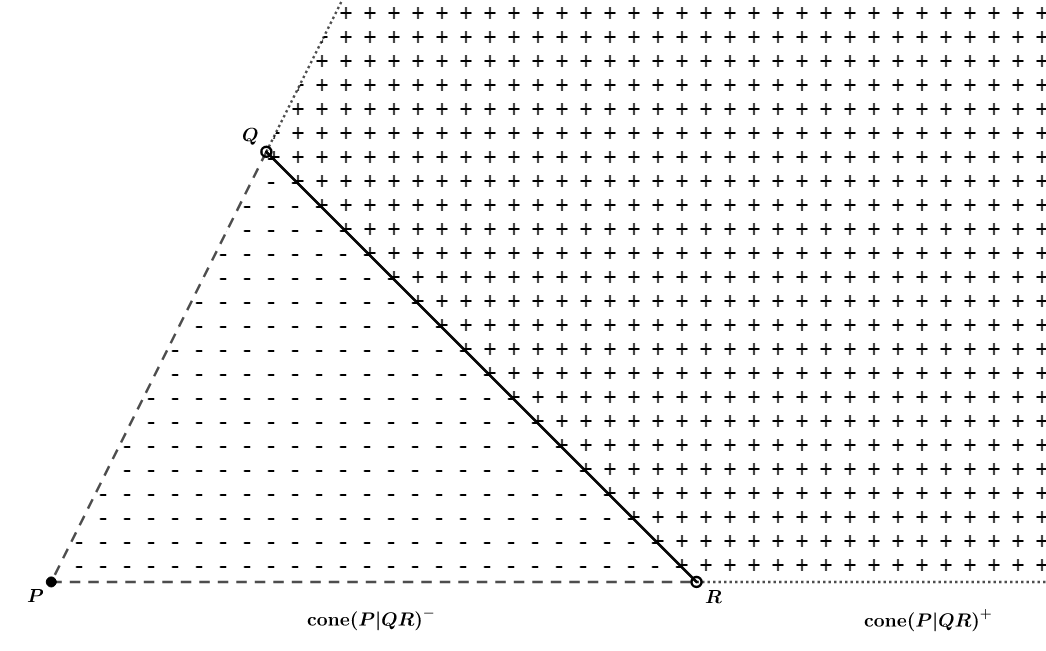
\includegraphics[width=0.75\linewidth]{figures/cones}
		\label{fig:cones}
	\end{figure}
	Let $B = \overline{P^1_BP^2_B}\in\mathcal B$ a barrier. In the following proposition, we give a sufficient condition to not include the edge $(P^{}_N, P^i_B)$ in $\EN$.
	
	\begin{prop}
		
		Let $B'=\overline{P^1_{B'}P^2_{B'}}\in\mathcal B$ and $\normalfont{\text{cone}}(P^i_B|P^1_{B'}P^2_{B'})^+$ the conical hull generated by these points. If
		$$N\subset\bigcup_{B'\in\mathcal B}\normalfont{\text{cone}}(P^i_B| P^1_{B'}P^2_{B'})^+,$$
		then $(P^{}_N, P^i_B)\not\in \EN$.
		
		%Let $B'=\overline{P^1_{B'}P^2_{B'}}\in\mathcal B$ and $Q(B')$ the intersection point of the straight lines that join points of $N$ and $B'$ that lies outside of the convex hull generated by thse line segments. Let $\normalfont{\text{cone}}(\{\overrightarrow{Q(B')P^1_N},\overrightarrow{Q(B')P^2_N}\})$ the conical hull of these vectors. If
		%$$B\subset\bigcup_{B'\in\mathcal B}\normalfont{\text{cone}}(\{\overrightarrow{Q(B')P^1_N},\overrightarrow{Q(B')P^2_N}\}),$$
		%then $(P^{}_N, P^i_{B})\not\in \EN$, $i=1,2$.
	\end{prop}
	\begin{proof}
		If $P_N\in N$, then there exists a $B'\in\mathcal B$ such that 
		$P_N\in \normalfont{\text{cone}}(P^i_B|P^1_{B'}P^2_{B'})^+$. Therefore, $\overline{P^i_B P^{}_N}\cap B'\neq\emptyset$ and $(P^{}_N, P^i_B)\not\in \EN$.
	\end{proof}
	
	One can easily check computationally the condition of the previous proposition by using the following procedure. First, we deal with the case where neighbourhoods are segments. Let $N = \overline{P^1_N P^2_N}$ be a line segment and $r_N$ be the straight line that contains the line segment $N$ represented as:
	
	$$r_N:P_N^1+\lambda\overrightarrow{P_N^1P_N^2},\qquad\lambda\in\mathbb R.$$
	
	
	\begin{algorithm}[H]
		\caption{Checking computationally whether $(P^{}_N, P^i_B)\not\in \EN$ when $N$ is a segment.}
		\label{alg:Algorithm1}
		\SetKwInOut{Input}{Initialization}\SetKwInOut{Output}{output}
		
		\Input{Let $P^i_B$ be the point of the edge $(P^{}_N, P^i_B)$ to check whether $(P^{}_N, P^i_B)\not\in \EN$.\\
			Set $points = \{P^1_N, P^2_N\}$, $lambdas=\{0, 1\}$.}
		% Set $LB=0$, $UB=+\infty$, $\bar z=z^0$.
		\For{$B''\in\mathcal B$}{
			\For{$j\in\{1, 2\}$}{
				Compute the straight line 
				$$r(P^i_B, P^j_{B''}) = P^i_B + \mu^j_{B''}\overrightarrow{P^i_BP^j_{B''}},$$ 
				that contains the points $P^i_B$ and $P^j_{B''}$. \\
				
				Intersect $r(P^i_B, P^j_{B''})$ and $r_N$ at the point $Q^j_{B''}$ and compute $			\overline{\mu}^j_{B''}$ such that 
				$$Q^j_{B''}=P_B^i + \overline{\mu}^j_{B''} \overrightarrow{P^i_BP^j_{B''}}.$$\\
				
				\If{$|\overline{\mu}^j_{B''}|\geq 1$}{
					Compute $\lambda^j_{B''}$ such that 
					$$Q^j_{B''}=P^1_N+\lambda^j_{B''}\overrightarrow{P^1_NP^2_N}.$$\\
					\If{$\overline{\mu}^j_{B''}\geq 1$}{
						Include $\lambda^j_{B''}$ in $lambdas$.}
					\Else{
						\If{$\lambda^j_{B''}\geq 0$}{
							Set $\lambda^j_{B''}=M<<0$ and include it in $lambdas$.}
						\Else{
							Set $\lambda^j_{B''}=M>>0$ and include it in $lambdas$.}
					}	
				}
			}
		}
		Order  the set $lambdas$ in non-decreasing order.\\
		If it is satisfied that
		\begin{align*}
			\min\{\lambda_{B'}^1, \lambda_{B'}^2\}\leq 0\leq\max\{\lambda_{B'}^1, \lambda_{B'}^2\},&\quad\text{ for some } B'\in\mathcal B,\\
			\min\{\lambda_{B'}^1, \lambda_{B'}^2\}\leq 1\leq\max\{\lambda_{B'}^1, \lambda_{B'}^2\},&\quad\text{ for some } B'\in\mathcal B,\\
			\min\{\lambda_{B'}^1, \lambda_{B'}^2\}\leq\lambda_{B''}^j\leq\max\{\lambda_{B'}^1, \lambda_{B'}^2\},&\quad\text{ for some } B'\in\mathcal B\setminus\{B''\},\quad\forall \lambda_{B''}^j\in lambdas\setminus\{M\},
		\end{align*}
		or
		$$
		\min\{\lambda_{B'}^1, \lambda_{B'}^2\}\leq 0, 1\leq\max\{\lambda_{B'}^1, \lambda_{B'}^2\},\quad\text{ for some } B'\in\mathcal B,
		$$
		then $(P^{}_N, P^i_B)\not\in \EN$.
		
	\end{algorithm}
	
	In Figure \ref{fig:algorithm1} an example of the Algorithm \ref{alg:Algorithm1} is described to check if there exists a rectilinear path that joins the solid point $P^i_B$ in the red barrier defined by the extreme points $P_B^i$ and $P_B^j$ with the segment $\segment{P^1_N}{P^2_N}$. First, the dashed straight lines $r(P^i_B, P^j_{B''})$  generated by $P^i_B$ and each point of the barrier are computed. Second, the straight line $r_N$ is determined by $P_N^1$ and $P_N^2$. Then, each of the straight lines $r(P^i_B, P^j_{B''})$ is intersected with $r_N$ obtaining the points $Q_1^1,\,Q_2^1,\,Q_1^2$ and $Q_2^2$. Each of these points has two associated parameter values $\mu$ and $\lambda$ with respect to the straight lines $r(P^i_B, P^j_{B''})$ and $r_N$, respectively. Finally, the points are ordered in nondecreasing sequence with respect to the $\lambda$ values. Since 
	$$
	M=\lambda_1^1 \leq 0, 1\leq\lambda_1^2=2,
	$$
	the segment $\segment{P_N^1}{P_N^2}$ is fully included in $\text{cone}(P_B^i|P_1^1P_1^2)^+$ and, therefore, $(P^i_B, P_N)$ is not included in $\EN$.
	
	\input{figures/Preprocessing - First case}
	
	Note that this algorithm also allows us to decide whether the drone can access a barrier point from any point in the neighbourhood $N$. It is enough to check in (15) that 
	$$0\not\in \left[\min\{\lambda_{B'}^1, \lambda_{B'}^2\},\max\{\lambda_{B'}^1, \lambda_{B'}^2\}\right]\quad\text{and}\quad 1\not\in \left[\min\{\lambda_{B'}^1, \lambda_{B'}^2\},\max\{\lambda_{B'}^1, \lambda_{B'}^2\}\right],\quad\forall B'\in\mathcal B.$$
	
	For the case where $N$ is an ellipse, the same rationale can be followed. The idea is to generate the largest line segment contained in the ellipse and to repeat the procedure in Algorithm \ref{alg:Algorithm1}. Let $F_1$ and $F_2$ be the focal points of $N$.
	
	\begin{algorithm}[H]
		\caption{Checking computationally whether $(P^{}_N, P^i_B)\not\in \EN$ when $N$ is an ellipse.}
		\label{alg:Algorithm2}
		\SetKwInOut{Input}{Initialization}\SetKwInOut{Output}{output}
		
		\Input{Let $P^i_B$ be the point whose edge $(P^i_B, P^{}_N)$ is going to check whether $(P^{}_N, P^i_B)\not\in \EN$.\\
			Set $points = \{\}$, $lambdas=\{\}$.}
		% Set $LB=0$, $UB=+\infty$, $\bar z=z^0$.}
	Compute the straight line $r(F^1, F^2)$.\\
	Intersect $r(F^1, F^2)$ and the boundary of $N$, $\partial N$, in the points $P_N^1$ and $P_N^2$. \\
	Include $P_N^1$ and $P_N^2$ in $points$. \\
	Apply Algorithm \ref{alg:Algorithm1}.
\end{algorithm}

\subsection{Valid inequalities}
This subsection is devoted to showing some results that adjust the big M constants that appear in the previous formulation, specifically, in constraints \eqref{eq:alphaC}, where modelling of the sign requires computing the lower and upper bounds $L$ and $U$, respectively. We are going to determine these bounds explicitly for the cases where the neighbourhoods are ellipses and segments.

Let $\overline{P^1_{B'}P^2_{B'}}=B'\in\B$ be a barrier, and $P_N\in N$. Let $\determinant{P_N}{P_{B'}^1}{P_{B'}^2}$ also be the determinant whose value must be bounded. Clearly, the solution of the following problem gives a lower bound of the determinant:
\begin{equation*}\label{eq:L-Problem}\tag{L-Problem}
	\overline{L}=\min_{P_N=(x,y)\in N}F(x,y):=\determinant{P^{}_N}{P_{B'}^1}{P_{B'}^2}=\left|
	\begin{array}{cc}
		P^{1}_{B'_x}-x & P^{2}_{B'_x}-x \\
		P^{1}_{B'_y}-y & P^{2}_{B'_y}-y
	\end{array}
	\right|.
\end{equation*}

\subsubsection{Lower and upper bounds when the neighbourhoods are line segments}
In this case, the segment whose endpoints are $P^1_{N}$ and $P^2_{N}$ can be expressed as the following convex set:
$$N=\{(x,y)\in\mathbb R^2:(x,y)=\mu P^1_{N}+(1-\mu)P^2_{N}, \; 0\leq\mu\leq1\}.$$
Since we optimise a linear function in a compact set, we can conclude that the objective function in \eqref{eq:L-Problem} achieves its minimum and maximum at the extreme points of $N$, that is, in $P^1_{N}$ and $P^2_{N}$. 

\subsubsection{Lower and upper bounds when the neighbourhoods are ellipses}\label{subsection:bounds}
The next case considered is that when $N$ is an ellipse, that is, $N$ is represented by the following inequality:
$$N=\{(x,y)\in\mathbb R^2:ax^2+by^2+cxy+dx+ey+f\leq 0\},$$
where $a, b, c, d, e, f$ are coefficients of the ellipse.
In extended form, we need to find:
\begin{mini*}
	{}{F(x, y)=\left|
		\begin{array}{cc}
			P^{1}_{B'_x}-x & P^{2}_{B'_x}-x \\
			P^{1}_{B'_y}-y & P^{2}_{B'_y}-y
		\end{array}
		\right|=xP^{1}_{B'_y}-xP^{2}_{B'_y}+yP^{2}_{B'_x}-yP^{1}_{B'_x}+P^{1}_{B'_x}P^{2}_{B'_y}-P^{1}_{B'_y}P^{2}_{B'_x},}
	{\label{eq:L-Ellipse}}{\tag{L-Ellipse}}
	\addConstraint{ax^2+by^2+cxy+dx+ey+f\leq 0.}
\end{mini*}
Since we minimise a linear function in a convex set, we can conclude that the extreme points are located in the frontier, so we can use the Lagrangian function to compute these points.
$$F(x,y;\lambda)=xP^{1}_{B'_y}-xP^{2}_{B'_y}+yP^{2}_{B'_x}-yP^{1}_{B'_x}+P^{1}_{B'_x}P^{2}_{B'_y}-P^{1}_{B'_y}P^{2}_{B'_x}+\lambda(ax^2+by^2+cxy+dx+ey+f).$$

$$\nabla F(x,y;\lambda)=0\Longleftrightarrow
\left\{\begin{array}{rcll}
	\frac{\partial F}{\partial x} & = & P^{1}_{B'_y}-P^{2}_{B'_y}+2ax\lambda+cy\lambda+d\lambda& =0,\\
	\frac{\partial F}{\partial y} & = & P^{2}_{B'_x}-P^{1}_{B'_x}+2by\lambda+cx\lambda+e\lambda& =0,\\
	\frac{\partial F}{\partial \lambda} & = & ax^2+by^2+cxy+dx+ey+f& =0.\\
\end{array}\right.$$
From the first two equations, we obtain the following:

$$\lambda = \frac{P^{2}_{B'_y}-P^{1}_{B'_y}}{2ax+cy+d}=\frac{P^{1}_{B'_x}-P^{2}_{B'_x}}{2by+cx+e}.$$

From this equality, we obtain the following general equation of the straight line:
\begin{align*}
	(P^{2}_{B'_y}-P^{1}_{B'_y})(2by+cx+e)-(P^{1}_{B'_x}-P^{2}_{B'_x})(2ax+cy+d)&=0,\\
	\left[c(P^2_{B'_y}-P^1_{B'_y})-2a(P^1_{B'_x}-P^2_{B'_x})\right]x+\left[2b(P^2_{B'_y}-P^1_{B'_y})-c(P^1_{B'_x}-P^2_{B'_x})\right]y+\left[e(P^2_{B'_y}-P^1_{B'_y})-d(P^1_{B'_x}-P^2_{B'_x})\right]&=0,\\
	\left[(2a, c)\cdot\overrightarrow{P^1_{B'}P^2_{B'}}\right]x+\left[(c, 2b)\cdot\overrightarrow{P^1_{B'}P^2_{B'}}\right]y+\left[(d, e)\cdot\overrightarrow{P^1_{B'}P^2_{B'}}\right]&=0,
	%	y\left[2b(P^{2}_{B'_y}-P^{1}_{B'_y})-c(P^{1}_{B'_x}-P^{2}_{B'_x})\right]&=\left[2a(P^{1}_{B'_x}-P^{2}_{B'_x})-c(P^{2}_{B'_y}-P^{1}_{B'_y})\right]x+\left[d(P^{1}_{B'_x}-P^{2}_{B'_x})-e(P^{2}_{B'_y}-P^{1}_{B'_y})\right],\\
	%	y&=\left[\frac{2a(P^{1}_{B'_x}-P^{2}_{B'_x})-c(P^{2}_{B'_y}-P^{1}_{B'_y})}{2b(P^{2}_{B'_y}-P^{1}_{B'_y})-c(P^{1}_{B'_x}-P^{2}_{B'_x})}\right]x+\left[\frac{d(P^{1}_{B'_x}-P^{2}_{B'_x})-e(P^{2}_{B'_y}-P^{1}_{B'_y})}{2b(P^{2}_{B'_y}-P^{1}_{B'_y})-c(P^{1}_{B'_x}-P^{2}_{B'_x})}\right],\\
	%	y&=mx+n.
\end{align*}
where $\cdot$ denotes the scalar product of two vectors. 
Solving the quadratic system:
$$
\left\{\begin{array}{rl}
	\left[(2a, c)\cdot\overrightarrow{P^1_{B'}P^2_{B'}}\right]x+\left[(c, 2b)\cdot\overrightarrow{P^1_{B'}P^2_{B'}}\right]y+\left[(d, e)\cdot\overrightarrow{P^1_{B'}P^2_{B'}}\right]&=0,\\
	ax^2+by^2+cxy+dx+ey+f& =0,\\
\end{array}\right.$$
they arise two solutions $x^{\pm}$ and $y^{\pm}$ that are evaluated in the objective function to obtain the lowest and highest value, respectively, according to $\LS{P_N^{}}{P_{B'}^1}{P_{B'}^2}$ and $\US{P_N^{}}{P_{B'}^1}{P_{B'}^2}$, respectively.
The reader may note that the same approach can be adopted to obtain the bounds for the rest of the determinants that appear in \eqref{eq:alphaC}.


\subsubsection{Variable Fixing}
In this subsection, the geometry of the problem is exploited to fix the variables. In particular, when a neighbourhood $N$ is in the half-space generated by a barrier $B$, the sign of the determinant $\determinant{P_N}{P_B^1}{P_B^2}$ does not change for any point $P_N\in N$. Therefore, a relevant number of variables $\alpha$ (hence $\beta$, $\gamma$, $\delta$ and $\varepsilon$) that model the sign of this determinant can be fixed `a priori'. It is sufficient to check whether both bounds $\LS{P_N^{}}{P_{B'}^1}{P_{B'}^2}$ and $\US{P_N^{}}{P_{B'}^1}{P_{B'}^2}$ computed in Subsection \ref{subsection:bounds} have the same sign or not. Figure \ref{fig:fixing_variables} shows an example where variables $\alpha$ can be fixed. Each of the blue neighbourhoods is completely contained in the half-spaces generated by the barrier, and $\alpha$ is fixed. However, the variable $\alpha$ corresponding to the orange neighbourhood depends on the half-space in which $P_N$ is located.

\pgfplotsset{compat=1.15}

\definecolor{ffvvqq}{rgb}{1,0.3333333333333333,0}
\definecolor{qqqqff}{rgb}{0,0,1}
\definecolor{ffqqqq}{rgb}{1,0,0}


\begin{figure}[!ht]
	\centering
\begin{tikzpicture}[line cap=round,line join=round,>=triangle 45,x=1cm,y=1cm, scale = 0.75]
\begin{axis}[
	x=0.1cm,y=0.1cm,
	axis lines=middle,
	xmin=-5,
	xmax=105,
	ymin=-5,
	ymax=105,
	xtick={-10,0,...,170},
	ytick={0,10,...,100},]
	\draw [line width=2pt,color=ffqqqq] (40,60)-- (60,50);
	\draw [rotate around={0:(20,25)},line width=2pt,color=qqqqff,fill=qqqqff,fill opacity=0.25] (20,25) ellipse (1cm and 1cm);
	\draw [rotate around={0:(70,80)},line width=2pt,color=qqqqff,fill=qqqqff,fill opacity=0.25] (70,80) ellipse (1cm and 1cm);
	\draw [rotate around={0:(80,35)},line width=2pt,color=ffvvqq,fill=ffvvqq,fill opacity=0.25] (80,35) ellipse (1cm and 1cm);
	\draw (40, 70) node[anchor=north west] {$\det(P_N|P_B^1P_B^2)\leq 0\Rightarrow \alpha(P_N|P_B^1P_B^2)\equiv 1$};
	\draw (1.5,15) node[anchor=north west] {$\det(P_N|P_B^1P_B^2)\geq 0\Rightarrow \alpha(P_N|P_B^1P_B^2)\equiv 0$};
	\draw [line width=2pt,dashed,color=ffqqqq,domain=-17.662128795895313:173.11488187960222] plot(\x,{(--1600-10*\x)/20});
	\begin{scriptsize}
		\draw [color=ffqqqq] (40,60) circle (2.5pt);
		\draw [color=ffqqqq] (60,50) circle (2.5pt);
	\end{scriptsize}
\end{axis}
\end{tikzpicture}
\caption{Fixing $\alpha$ variables when the whole neighborhood lies in one of the half-spaces the generated by the barrier}
\label{fig:fixing_variables}
\end{figure}

\section{Computational experiments}\label{section:experiments}
This section is devoted to studying the performance of \eqref{form:H-TSPHN} and \eqref{form:H-TSPN} formulations proposed in Section \ref{section:formulations}. In the first subsection, the procedure for generating the considered random instances is described. The second subsection details the experiments that have been conducted. The third subsection reports the results obtained in these experiments.

\subsection{Data generation}
%To generate the instances of our experiments, it is necessary that these instances verify the assumptions \ref{A1}-\ref{A4} stated in the Section \ref{section:description}. 

To generate the instances of our experiments, we assume assumptions \ref{A1}-\ref{A4} stated in Section \ref{section:description}. The following proposition gives an upper bound for the number of balls that can be generated given an instance with $n=|\mathcal B|$ barriers:

%		\JP{	
	%		\begin{prop}
		%			Under the hypothesis that balls are \CV{not} visible among them, the maximum number of balls that can be considered in \TSPHN \ is $O(n^2)$.
		%		\end{prop}
	%		\begin{proof}
		%			The proof is based on the properties of the visibility graph $VG(\cal B)$ of the configuration of barriers in $\cal B$:  It is clear that the maximum number of balls coincides with the number of faces, $f_{VG(\cal B)}$, of $VG(\cal B)$.  Recall that the number of vertices in $\cal B$ is $n$. Next, by the Euler formula, the number of faces $f_{VG(\cal B)}$ is $2+E_{VG(\cal B)}-n$. Since $E_{VG(\cal B)}=O(n^2)$, it follows that $f_{VG(\cal B)}=O(n^2)$.
		%		\end{proof}
	%	}


\begin{prop}
	Under assumptions \ref{A1}-\ref{A4}, the maximum number of balls that can be considered in \TSPHN \ is $O(n^2)$.
\end{prop}
\begin{proof}
	The proof is based on the properties of the visibility graph $VG(\cal B)$ of the barrier configuration in $\cal B$ \citep{mitchell_shortest_2017}:  It is clear that the maximum number of balls coincides with the number of faces, $f_{VG(\cal B)}$, of $VG(\cal B)$.  Recall that the number of vertices in $\cal B$ is $n$. Next, by the Euler formula, the number of faces $f_{VG(\cal B)}$ is $2+E_{VG(\cal B)}-n$. Since $E_{VG(\cal B)}=O(n^2)$, it follows that $f_{VG(\cal B)}=O(n^2)$.
\end{proof}

Algorithm \ref{alg:Algorithm3} describes a general way to construct instances where neighbourhoods are balls.

%	\begin{algorithm}[H]
	%		\caption{Generation of instances when the neighbourhoods are balls}
	%		\label{alg:Algorithm3}
	%		\SetKwInOut{Input}{Initialization}\SetKwInOut{Output}{output}
	%		
	%		\Input{Let $|\mathcal N|$ be the number of neighbourhoods to generate. Let $r_{\text{init}}=10$ be half of the initial length of the barriers.
		%			Set $\mathcal N = \{\}$; $points=\{\}$; $\mathcal B=\{\overline{(0, 0)(100, 0)}, \overline{(100, 0)(100, 100)}, \overline{(100, 100)(0, 100)}, \overline{(0, 100)(0, 0)}\}$.}
	%		% Set $LB=0$, $UB=+\infty$, $\bar z=z^0$.
	%		Generate $|\mathcal N|$ points uniformly distributed in the square $[0, 100]^2$ and include them in $points$. \\
	%		%\While{There does not exist a barrier that separates each pair of points}{
		%			\For{$P, P'\in points$}{
			%				\If{$\overline{PP'}\cap B=\emptyset,\;\forall B\in\mathcal B$}{
				%					Compute $\overrightarrow{d}=\overrightarrow{PP'}$.\\
				%					Compute $M = P + \frac 1 2 \overrightarrow{d}$.\\
				%					Compute the unitary vector $\overrightarrow{n_u}$ perpendicular to $\overrightarrow{d}$.\\
				%					Set $r = r_{\text{init}}$. \\
				%					Generate the barrier $B(r)=\overline{P_B^{+} P_B^{-}}$ where
				%					$P_B^{\pm}=M \pm r\overrightarrow{n_u}.$\\
				%					\While{$B(r)\cap B'\neq\emptyset$ for some $B'\in\mathcal B$}{
					%						Set $r := r / 2$. \\
					%						Generate the barrier $B(r)$.
					%					}
				%					
				%					Include $B(r)$ in $\mathcal B$.
				%					
				%					
				%				}
			%			}
		%			\For{$P\in points$}{
			%				Set $r_{\text{max}}=\min_{\{P_B\in B: B \in\mathcal B\}} d(P, P_B).$\\
			%				Generate a random $radii$ uniformly distributed in the interval $\left[\frac 1 2 r_{\text{max}}, r_{\text{max}}\right]$.\\
			%				Set the ball $N$ whose centre is $P$ and radii is $radii$. \\
			%				Include $N$ in $\mathcal N$.
			%			}
		%			%}
	%	\end{algorithm}

\begin{algorithm}[H]
	\caption{General scheme of the instances generation}
	\label{alg:Algorithm3}
	\SetKwInOut{Input}{Initialization}\SetKwInOut{Output}{output}
	
	\Input{Let $|\mathcal N|$ be the number of neighbourhoods to generate. \\
		%		Let $r_{\text{init}}$ be \CV{the} half of the initial length of the barriers. \\
		Let $R = [LB_x, UB_x]\times[LB_y, UB_y]\subseteq\mathbb R^2$ be the rectangle where centers will be generated. \\
		Set $points=\{\}$; $\mathcal B=\{\}$; $\mathcal N = \{\}$.}
	% Set $LB=0$, $UB=+\infty$, $\bar z=z^0$.
	Generate $|\mathcal N|$ points uniformly distributed in $R$ and include them in $points$. \\
	Generate pairwise disjoint barriers that separate the points and include them in $\mathcal B$. \\
	Generate neighbourhoods around $points$ and include them in $\mathcal N$. 
\end{algorithm}


\subsubsection*{Barriers generation}
In this subsection, we focus on how to generate line segments located in general position without crossings. The idea is to build bisectors that separate each pair of points in the set $points$. The initial length of each bisector is $r_{\text{init}}$. This length is reduced until it does not intersect any of the previously generated line segments. The Algorithm \ref{alg:Algorithm4} reports the pseudocode to generate barriers.

\begin{algorithm}[H]
	\caption{Generation of the barriers}
	\label{alg:Algorithm4}
	\SetKwInOut{Input}{Initialization}\SetKwInOut{Output}{output}
	
	\Input{Let $points$ be the set already randomly uniformly generated in $R$. \\
		Let $r_{\text{init}}$ be one half of the initial length of the barriers. \\
		Set $\mathcal B=\{\}$.}
	\For{$P, P'\in points$}{
		\If{$\overline{PP'}\cap B=\emptyset,\;\forall B\in\mathcal B$}{
			Compute $\overrightarrow{d}=\overrightarrow{PP'}$.\\
			Compute $M = P + \frac 1 2 \overrightarrow{d}$.\\
			Compute the unitary vector $\overrightarrow{n_u}$ perpendicular to $\overrightarrow{d}$.\\
			Set $r = r_{\text{init}}$. \\
			Generate the barrier $B(r)=\overline{P_B^{+} P_B^{-}}$ where
			$P_B^{\pm}=M \pm r\overrightarrow{n_u}.$\\
			\While{$B(r)\cap B'\neq\emptyset$ for some $B'\in\mathcal B$}{
				Set $r := r / 2$. \\
				Generate the barrier $B(r)$.}
			
			Include $B(r)$ in $\mathcal B$.	}}
\end{algorithm}

\subsubsection*{Neighbourhood generation}
Once the set of points and barriers are generated, the neighbourhoods are created using two different sizes:
\begin{itemize}
	\item \textbf{Randomly-sized neighbourhoods:} that do not intersect barriers and verify \ref{A4}. 
	\item \textbf{Fixed-sized neighbourhoods:} that can cross barriers and are not required to assume \ref{A4}. 
\end{itemize}
The first case is used to study the performance of the models \TSPHN \ and \TSPN \ proposed in the article when the neighbourhoods are circles or line segments. The following procedure describes the pseudocode to create circles.

\begin{algorithm}[H]
	\caption{Generation of randomly-sized circles}
	\label{alg:Algorithm5}
	\SetKwInOut{Input}{Initialization}\SetKwInOut{Output}{output}
	
	\Input{Let $points$ be the set randomly, uniformly generated in $R$. \\
		Let $\mathcal B$ be the barriers already generated.\\
		Set $\mathcal N=\{\}$.}
	\For{$P\in points$}{
		Set $r_{\text{max}}=\min_{\{P_B\in B: B \in\mathcal B\}} d(P, P_B).$\\
		Generate a random $radii$ uniformly distributed in the interval $\left[\frac 1 2 r_{\text{max}}, r_{\text{max}}\right]$.\\
		Set the ball $N$ whose centre is $P$ and radii is $radii$. \\
		Include $N$ in $\mathcal N$.}
	%}
\end{algorithm}

The line segments instances are generated by randomly selecting two diametrically opposite points in the boundary of the balls instances obtained with Algorithm \ref{alg:Algorithm5}.


The second case focuses on the effectiveness of the exact model for the \TSPN \ in terms of \emph{overlapping ratio} of the circles. This ratio, introduced in \cite{mennell_heuristics_2009}, is calculated by dividing the average radius of the neighbourhood sets by the length of the longest side of $R$. \cite{mennell_heuristics_2009} shows that the higher the overlaping ratio, the higher the difficulty of the instance. Algorithm \ref{alg:Algorithm5} is slightly modified by setting a fixed value for $radii$, based on instances considered in \cite{behdani_integer-programming-based_2014}.


%	To generate the instances when the neighbourhoods are segments, we can take the balls built in the previous procedure and draw a random angle that determines which point and its diametrically opposite point are selected as the endpoints of the line segment.

% \textcolor{red}{Quizás evitar el uso $n$ sea adecuado para evitar confusiones}
\subsection{Configuration of the experiments}
In this work, two experiments are designed to study the behaviour of the models \TSPHN \ and \TSPN. In the first experiment, we generate five instances for each number of randomly-sized neighbourhoods in $|\mathcal N|\in\{5, 10, 20, 30, 50, 60, 65, 70, 75, 80, 100\}$ within $R=[0,100]\times[0, 100]$. These neighbourhoods are balls and line segments that have been created using the Algorithm \ref{alg:Algorithm5}. For each instance, we run the models with and without strengthening the formulations.

In the second experiment, based on \cite{behdani_integer-programming-based_2014}, we generate five instances with a number $N$ in $|\mathcal N|\in\{6, 8, 10, 12, 14, 16, 18, 20\}$ of fixed circles. The centres are drawn in $R=[0, 0]\times[16, 10]$. The fixed $radii$ considered are $0.25$, $0.5$, and $1$. Therefore, the overlap ratios are $0.015625$, $0.03125$ and $0.0625$, respectively. We run \TSPN \ with strengthening to see the performance of our methods when neighbourhoods overlap.

Formulations are coded in Python 3.9.2 (\citet{van_rossum_python_2009}) and solved in Gurobi 9.1.2 (\citet{gurobi_optimization_llc_gurobi_2022}) on an AMD® Epyc 7402p 8-core processor.

The values obtained by solver that are reported in our tables are:

\begin{itemize}
\item \boldsymbol{$\#Found$}: number of instances in which the solver finds a feasible solution.
\item \boldsymbol{$Gap$}: gap between the best incumbent solution with respect to the best bound found by the solver. It is computed as $Gap=(upper\, bound - lower\, bound)/lower\, bound$.
\item \boldsymbol{$Time_{model}$}: time spent by the solver to obtain the best solution found.
\item \boldsymbol{$Time_{prepro}$}: time spent by Python to set up the model, including the strengthening of the formulation.
\item \boldsymbol{$Time_{total}$}: overall time to solve the model.
\end{itemize}

For all the experiments, a time limit of 1 hour of solver time was set in the branch-and-bound procedure.



\subsection{Results of the experiments}
We report the results of the first experiment in Table \ref{table:results}. The layout is organised in 3 blocks of columns. The first block describes the parameters of the problem: number of neighbourhoods $|\mathcal{N}|$, if \ref{A4} is assumed or not (\TSPHN\xspace vs \TSPN), if strengthening is considered, and the number of barriers. The second and third blocks describe the average results obtained with the solver for circles and segments, respectively. 

%	typology of neighbourhood used in the experiment (Balls or Segments), the third one (strengthening)  informs whether the strengthening is being applied or not (True or False). The next three blocks include information  on the number of barriers ($|\mathcal{B}|$), the  gap at termination (Gap) defined as $Gap=(upper\, bound - lower\, bound)/lower\, bound$, and the computing time (Runtime). The block $|\mathcal{B}|$ indicates the minimum and maximum number of barriers considered in each of the instances for each fixed number $|\mathcal{N}|$ of neighbours. The block Gap contains three columns reporting the average (mean), minimum (min), and maximum (max) gaps of the ten instances considered for each combination of parameters. Analogously, the block Runtime also includes three columns reporting the average (mean), minimum (min) and maximum (max) computing time of the ten instances considered for each combination of parameters.
%	By rows, Table \ref{table:results} reports results for instances with a number of neigbourhoods $|\mathcal{N}|$ in the set $\{5,10,20,30,50,80,100\}$. For each value of $|\mathcal{N}|$  we report results for two typologies of neigbourhoods, namely Balls and Segments, without strengthening (False) and with strengthening (True).


Analysing the results in Table \ref{table:results}, we first observe that solving the problem considering balls as neighbourhoods is harder than solving with segments. Next, we also observe that this approach solves to optimality all instances for circles up to $|\mathcal{N}|=30$ with strengthening for the \TSPHN \ problem. However, if we do not strengthen the formulation, the solver always reports gap for all the instances with circles. The same behaviour can be seen for the \TSPN \xspace up to $|\mathcal{N}|=30$. Nevertheless, for sizes $|\mathcal{N}|$ in 50-75, both formulations start to differ in the number of instances in which the solver can find a feasible solution. For the \TSPHN, the reader may observe that strengthening does not improve the gap within the time limit. However, in the \TSPN, strengthening does increase the number of instances in which the solver finds a solution and the fraction of gaps certified after the execution time. Anyway, whenever a feasible solution is found, the maximum average gap that is reported with strengthening is $0.35$. Finally, for sizes 80 and 100, the solver cannot find any solution for any of the models, regardless of whether strengthening is considered or not. In terms of execution time, we can conclude that strengthening always improves both the time to obtain the optimal solution ($\boldsymbol{Time_{model}}$) and the time the computer takes to load all the variables and constraints of the model ($\boldsymbol{Time_{prepro}}$). This difference is more appreciable in the \TSPHN, as the reader can notice in the aggregation of these two columns in ($\boldsymbol{Time_{total}}$). This fact can be explained in terms of the number of barriers: the higher the number of barriers, the larger the number of variables that can be fixed beforehand. On the other hand, we can observe that Gurobi can report the optimal solution for almost all segment instances generated by solving the strengthened versions of the \TSPHN\xspace and \TSPN. In addition, the time spent to solve all these instances is lower than the time limit. However, the time to load and strengthen the model is very similar to that for circle instances.

In Figures \ref{fig:Fig4} and \ref{fig:Fig5}, the reader can compare, at a glance, the time that the solver spent to obtain the best solution found and the gap between this solution and the best bound found by the solver. We can conclude that strengthening improves significantly the time spent by Gurobi to get the optimal solution and instances with circles are harder to be solved than those with segments, in terms of time and final gap.

%	In addition, both typologies of instances, up to $|\mathcal{N}|=50$, are almost solved by obtaining a small average gap. %and also almost all for balls leaving always a gap less than or equal to  1\%. 
%	We also observe that the use of strengthening helps in solving the instances since in those cases where they are not solved to optimality the gap and the runtime are reduced. The situation for $|\mathcal{N}|\in \{80,100\}$ is slightly different. For $|\mathcal{N}|=80$ and balls as neighbourhoods, the strengthening time takes more than an hour so that no results can be reported whereas without strengthening the formulations are always able to find solutions with average gaps of ($\le 0.6$) within one hour of computing time.  % For segments we see that the use of strengthening helps and the gaps are smaller within the time limit. 
%	Finally, for the case of $|\mathcal{N}|=100$ balls as neighbourhoods, none of the configurations with or without strengthening is capable to find a feasible solution in 3600 seconds. The behaviour is different for segments. In this case, both configurations provide feasible solutions. In the last case, the use of strengthening is rather heavy and consumes most of the 3600 seconds of computing time. This can be observed in the final gaps. The case without strengthening reports better gaps, as leaving more time to the solver to find better solutions, and the average gap is $0.53$ rather than $0.81$ for the case with strengthening.
%	
%% Table generated by Excel2LaTeX from sheet 'Hoja1'
%\begin{table}[htbp]
%	\centering
%	\caption{Add caption}
%	\resizebox{\textwidth}{!}{
%	\begin{tabular}{|c|c|c||cc|ccc|ccc|}
	%		\hline
	%		$\bm{|\mathcal N|}$ & \textbf{Typology} & \textbf{strengthening} & \multicolumn{2}{c|}{$\bm{|\mathcal B|}$} & \multicolumn{3}{c|}{\textbf{Gap}} & \multicolumn{3}{c|}{\textbf{Runtime}} \bigstrut[t]\\
	%		&       &       & \textbf{min} & \textbf{max} & \textbf{mean} & \textbf{min} & \textbf{max} & \textbf{mean} & \textbf{min} & \textbf{max} \bigstrut[b]\\
	%		\hline
	%		\hline
	%		\multirow{4}[4]{*}{5} & \multirow{2}[2]{*}{Ball} & False & 8     & 11    & 0     & 0     & 0     & 2.46  & 1.2   & 8.05 \bigstrut[t]\\
	%		&       & True  & 8     & 11    & 0     & 0     & 0     & 1.63  & 0.81  & 2.49 \bigstrut[b]\\
	%		\cline{2-11}          & \multirow{2}[2]{*}{Segment} & False & 8     & 11    & 0     & 0     & 0     & 1.35  & 0.82  & 2.52 \bigstrut[t]\\
	%		&       & True  & 8     & 11    & 0     & 0     & 0     & 1.09  & 0.79  & 1.41 \bigstrut[b]\\
	%		\hline
	%		\hline
	%		\multirow{4}[4]{*}{10} & \multirow{2}[2]{*}{Ball} & False & 15    & 21    & 0     & 0     & 0     & 13.43 & 7.85  & 27.68 \bigstrut[t]\\
	%		&       & True  & 15    & 21    & 0     & 0     & 0     & 6.22  & 3.61  & 11.85 \bigstrut[b]\\
	%		\cline{2-11}          & \multirow{2}[2]{*}{Segment} & False & 15    & 21    & 0     & 0     & 0     & 7.41  & 5.04  & 9.23 \bigstrut[t]\\
	%		&       & True  & 15    & 21    & 0     & 0     & 0     & 4.54  & 3.15  & 5.7 \bigstrut[b]\\
	%		\hline
	%		\hline
	%		\multirow{4}[4]{*}{20} & \multirow{2}[2]{*}{Ball} & False & 35    & 40    & 0     & 0     & 0     & 132.22 & 58.21 & 225.89 \bigstrut[t]\\
	%		&       & True  & 35    & 40    & 0     & 0     & 0     & 45.86 & 20.32 & 104.49 \bigstrut[b]\\
	%		\cline{2-11}          & \multirow{2}[2]{*}{Segment} & False & 35    & 40    & 0     & 0     & 0     & 97.25 & 40.06 & 166.67 \bigstrut[t]\\
	%		&       & True  & 35    & 40    & 0     & 0     & 0     & 38.47 & 15.77 & 66.05 \bigstrut[b]\\
	%		\hline
	%		\hline
	%		\multirow{4}[4]{*}{30} & \multirow{2}[2]{*}{Ball} & False & 49    & 60    & 0     & 0     & 0     & 373.32 & 246.51 & 639.97 \bigstrut[t]\\
	%		&       & True  & 49    & 60    & 0     & 0     & 0     & 127.15 & 53.08 & 219.85 \bigstrut[b]\\
	%		\cline{2-11}          & \multirow{2}[2]{*}{Segment} & False & 49    & 60    & 0     & 0     & 0     & 414.11 & 156.76 & 979.68 \bigstrut[t]\\
	%		&       & True  & 49    & 60    & 0     & 0     & 0     & 112.68 & 50.66 & 182.82 \bigstrut[b]\\
	%		\hline
	%		\hline
	%		\multirow{4}[4]{*}{50} & \multirow{2}[2]{*}{Ball} & False & 79    & 91    & 0     & 0     & 0.01  & 1634.35 & 603.48 & 3605.13 \bigstrut[t]\\
	%		&       & True  & 79    & 91    & 0     & 0     & 0     & 553.93 & 181.13 & 1599.18 \bigstrut[b]\\
	%		\cline{2-11}          & \multirow{2}[2]{*}{Segment} & False & 79    & 91    & 0     & 0     & 0.01  & 1618.95 & 855.65 & 3604.93 \bigstrut[t]\\
	%		&       & True  & 79    & 91    & 0     & 0     & 0     & 523.08 & 152.08 & 1548.64 \bigstrut[b]\\
	%		\hline
	%		\hline
	%		\multirow{4}[4]{*}{80} & \multirow{2}[2]{*}{Ball} & False & 125   & 145   & -     & -     & -     & -     & -     & - \bigstrut[t]\\
	%		&       & True  & 125   & 145   & 0.01  & 0     & 0.02  & 3110.68 & 1976.01 & 3601.13 \bigstrut[b]\\
	%		\cline{2-11}          & \multirow{2}[2]{*}{Segment} & False & 125   & 145   & -     & -     & -     & -     & -     & - \bigstrut[t]\\
	%		&       & True  & 125   & 145   & 0.01  & 0     & 0.03  & 2835.09 & 1663.53 & 3601.26 \bigstrut[b]\\
	%		\hline
	%	\end{tabular}}%
%	\label{tab:addlabel}%
%\end{table}%

%	% Table generated by Excel2LaTeX from sheet 'Hoja1'
%	\begin{table}[htbp]
%		\centering
%		\caption{Table of computational results obtained with the formulation \eqref{form:H-TSPHN}}
%		\resizebox{\textwidth}{!}{
	%			\begin{tabular}{|c|c|c||cc|ccc|ccc|}
		%				\hline
		%				$\bm{|\mathcal N|}$ & \textbf{neighbourhood} & \textbf{strengthening} & \multicolumn{2}{c|}{$\bm{|\mathcal B|}$} & \multicolumn{3}{c|}{\textbf{Gap}} & \multicolumn{3}{c|}{\textbf{Runtime}} \bigstrut[t]\\
		%				&       &       & \textbf{min} & \textbf{max} & \textbf{mean} & \textbf{min} & \textbf{max} & \textbf{mean} & \textbf{min} & \textbf{max} \bigstrut[b]\\
		%				\hline
		%				\hline
		%				\multirow{4}[4]{*}{5} & \multirow{2}[2]{*}{Ball} & False & \multirow{4}[4]{*}{8} & \multirow{4}[4]{*}{11} & 0.05  & 0     & 0.55  & 371.84 & 2.96  & 3600 \bigstrut[t]\\
		%				&       & True  &       &       & 0     & 0     & 0     & 3.46  & 1.4   & 13 \bigstrut[b]\\
		%				\cline{2-3}\cline{6-11}          & \multirow{2}[2]{*}{Segment} & False &       &       & 0.08  & 0     & 0.49  & 1085.48 & 0.68  & 3600 \bigstrut[t]\\
		%				&       & True  &       &       & 0     & 0     & 0     & 1.44  & 0.6   & 2.46 \bigstrut[b]\\
		%				\hline
		%				\hline
		%				\multirow{4}[4]{*}{10} & \multirow{2}[2]{*}{Ball} & False & \multirow{4}[4]{*}{15} & \multirow{4}[4]{*}{21} & 0.17  & 0     & 0.86  & 998.71 & 59.09 & 3600 \bigstrut[t]\\
		%				&       & True  &       &       & 0     & 0     & 0     & 36.66 & 10.72 & 87.29 \bigstrut[b]\\
		%				\cline{2-3}\cline{6-11}          & \multirow{2}[2]{*}{Segment} & False &       &       & 0.33  & 0     & 0.86  & 1460.31 & 16.78 & 3600 \bigstrut[t]\\
		%				&       & True  &       &       & 0     & 0     & 0     & 8.53  & 2.66  & 12.25 \bigstrut[b]\\
		%				\hline
		%				\hline
		%				\multirow{4}[4]{*}{20} & \multirow{2}[2]{*}{Ball} & False & \multirow{4}[4]{*}{35} & \multirow{4}[4]{*}{40} & 0.06  & 0.02  & 0.1   & 3600  & 3600  & 3600 \bigstrut[t]\\
		%				&       & True  &       &       & 0     & 0     & 0.01  & 1424.85 & 140.54 & 3600 \bigstrut[b]\\
		%				\cline{2-3}\cline{6-11}          & \multirow{2}[2]{*}{Segment} & False &       &       & 0     & 0     & 0.02  & 1430.13 & 166.89 & 3600 \bigstrut[t]\\
		%				&       & True  &       &       & 0     & 0     & 0     & 198.9 & 30.75 & 426.55 \bigstrut[b]\\
		%				\hline
		%				\hline
		%				\multirow{4}[4]{*}{30} & \multirow{2}[2]{*}{Ball} & False & \multirow{4}[4]{*}{49} & \multirow{4}[4]{*}{60} & 0.12  & 0     & 0.93  & 3566.2 & 3246.53 & 3600 \bigstrut[t]\\
		%				&       & True  &       &       & 0     & 0     & 0.02  & 2146.17 & 314.65 & 3600 \bigstrut[b]\\
		%				\cline{2-3}\cline{6-11}          & \multirow{2}[2]{*}{Segment} & False &       &       & 0     & 0     & 0.01  & 2119.06 & 315.56 & 3600 \bigstrut[t]\\
		%				&       & True  &       &       & 0     & 0     & 0     & 1140.02 & 353.73 & 3209.94 \bigstrut[b]\\
		%				\hline
		%				\hline
		%				\multirow{4}[4]{*}{50} & \multirow{2}[2]{*}{Ball} & False & \multirow{4}[4]{*}{79} & \multirow{4}[4]{*}{91} & 0.09  & 0.02  & 0.19  & 3600  & 3600  & 3600 \bigstrut[t]\\
		%				&       & True  &       &       & 0.08  & 0.01  & 0.21  & 3600  & 3600  & 3600 \bigstrut[b]\\
		%				\cline{2-3}\cline{6-11}          & \multirow{2}[2]{*}{Segment} & False &       &       & 0.02  & 0.01  & 0.09  & 3600  & 3600  & 3600 \bigstrut[t]\\
		%				&       & True  &       &       & 0.02  & 0     & 0.1   & 2956.24 & 2053.62 & 3600 \bigstrut[b]\\
		%				\hline
		%				\hline
		%				\multirow{4}[4]{*}{80} & \multirow{2}[2]{*}{Ball} & False & \multirow{4}[4]{*}{125} & \multirow{4}[4]{*}{145} & 0.6   & 0.42  & 0.79  & 3600  & 3600  & 3600 \bigstrut[t]\\
		%				&       & True  &       &       & -     & -     & -     & -     & -     & - \bigstrut[b]\\
		%				\cline{2-3}\cline{6-11}          & \multirow{2}[2]{*}{Segment} & False &       &       & 0.16  & 0.03  & 0.62  & 3600  & 3600  & 3600 \bigstrut[t]\\
		%				&       & True  &       &       & 0.61  & 0.01  & 1     & 3600  & 3600  & 3600 \bigstrut[b]\\
		%				\hline
		%				\hline
		%				\multirow{4}[4]{*}{100} & \multirow{2}[2]{*}{Ball} & False & \multirow{4}[4]{*}{156} & \multirow{4}[4]{*}{178} & -     & -     & -     & -     & -     & - \bigstrut[t]\\
		%				&       & True  &       &       & -     & -     & -     & -     & -     & - \bigstrut[b]\\
		%				\cline{6-11}          & \multirow{2}[2]{*}{Segment} & False &       &       & 0.53  & 0.02  & 0.99  & 3600  & 3600  & 3600 \bigstrut[t]\\
		%				&       & True  &       &       & 0.81  & 0.5   & 1     & 3600  & 3600  & 3600 \bigstrut[b]\\
		%				\hline
		%		\end{tabular}}%
%		\label{table:results}%
%	\end{table}%

%	The same behaviour is also observed in Figure 9. The left subfigure reports the boxplot diagram for the experiments with segments as neighbourhoods, whereas the right one reports the boxplot diagram for balls as neighbourhoods. We see that strengthening always helps since the corresponding boxes are below those without strengthening, whenever the problems are solved well. Moreover,  we also observe in those cases where the model solves the instances  $|\mathcal{N}|\le 50$, that the problem with balls is harder than with segments since the boxes in the left subfigure are below the ones in the right subfigure.
%	





% \DeclareUnicodeCharacter{2212}{−}
% \usepgfplotslibrary{groupplots}
\usetikzlibrary{patterns,shapes.arrows}
\pgfplotsset{compat=newest}

\definecolor{darkslategray38}{RGB}{38,38,38}
\definecolor{darkslategray76}{RGB}{76,76,76}
\definecolor{lavender234234242}{RGB}{234,234,242}
\definecolor{peru20313699}{RGB}{203,136,99}
\definecolor{steelblue88116163}{RGB}{88,116,163}

\begin{figure}[h!]
    \centering
\begin{tikzpicture}[scale=0.9]

\definecolor{color0}{rgb}{0.917647058823529,0.917647058823529,0.949019607843137}
\definecolor{color1}{rgb}{0.347058823529412,0.458823529411765,0.641176470588235}
\definecolor{color2}{rgb}{0.798529411764706,0.536764705882353,0.389705882352941}

\begin{axis}[
axis background/.style={fill=color0},
axis line style={white},
tick align=outside,
title={Neighborhood = Segment},
x grid style={white},
xtick pos = left,
ytick pos = left,
xlabel={$|\mathcal N|$},
% xmajorticks=false,
xmin=-0.5, xmax=6.5,
xtick style={color=white!15!black},
xtick={0,1,2,3,4,5,6},
xticklabels={5, 10, 20, 30, 50, 80, 100},
y grid style={white},
ylabel={Runtime},
ymajorgrids,
% ymajorticks=false,
ymin=-0.05, ymax= 7200,
log basis y={10},
ymode = log,
ytick style={color=white!15!black},
%ytick={-0.2,0,0.2,0.4,0.6,0.8,1,1.2},
%yticklabels={−0.2,0.0,0.2,0.4,0.6,0.8,1.0,1.2},
legend pos = south east
]
\path [draw=darkslategray76, fill=steelblue88116163, semithick]
(axis cs:-0.396,1.32029229402542)
--(axis cs:-0.004,1.32029229402542)
--(axis cs:-0.004,2321.5214869976)
--(axis cs:-0.396,2321.5214869976)
--(axis cs:-0.396,1.32029229402542)
--cycle;
\path [draw=darkslategray76, fill=peru20313699, semithick]
(axis cs:0.004,0.867011845111847)
--(axis cs:0.396,0.867011845111847)
--(axis cs:0.396,1.71693199872971)
--(axis cs:0.004,1.71693199872971)
--(axis cs:0.004,0.867011845111847)
--cycle;
\path [draw=darkslategray76, fill=steelblue88116163, semithick]
(axis cs:0.604,22.0478292107582)
--(axis cs:0.996,22.0478292107582)
--(axis cs:0.996,3600.1058292985)
--(axis cs:0.604,3600.1058292985)
--(axis cs:0.604,22.0478292107582)
--cycle;
\path [draw=darkslategray76, fill=peru20313699, semithick]
(axis cs:1.004,5.35795325040817)
--(axis cs:1.396,5.35795325040817)
--(axis cs:1.396,11.317633330822)
--(axis cs:1.004,11.317633330822)
--(axis cs:1.004,5.35795325040817)
--cycle;
\path [draw=darkslategray76, fill=steelblue88116163, semithick]
(axis cs:1.604,336.735125482082)
--(axis cs:1.996,336.735125482082)
--(axis cs:1.996,2661.89892309904)
--(axis cs:1.604,2661.89892309904)
--(axis cs:1.604,336.735125482082)
--cycle;
\path [draw=darkslategray76, fill=peru20313699, semithick]
(axis cs:2.004,124.047738432884)
--(axis cs:2.396,124.047738432884)
--(axis cs:2.396,243.347989618778)
--(axis cs:2.004,243.347989618778)
--(axis cs:2.004,124.047738432884)
--cycle;
\path [draw=darkslategray76, fill=steelblue88116163, semithick]
(axis cs:2.604,758.177148163319)
--(axis cs:2.996,758.177148163319)
--(axis cs:2.996,3601.57422971725)
--(axis cs:2.604,3601.57422971725)
--(axis cs:2.604,758.177148163319)
--cycle;
\path [draw=darkslategray76, fill=peru20313699, semithick]
(axis cs:3.004,415.898770868778)
--(axis cs:3.396,415.898770868778)
--(axis cs:3.396,1199.34626537561)
--(axis cs:3.004,1199.34626537561)
--(axis cs:3.004,415.898770868778)
--cycle;
\path [draw=darkslategray76, fill=steelblue88116163, semithick]
(axis cs:3.604,3601.05894333124)
--(axis cs:3.996,3601.05894333124)
--(axis cs:3.996,3606.46183502674)
--(axis cs:3.604,3606.46183502674)
--(axis cs:3.604,3601.05894333124)
--cycle;
\path [draw=darkslategray76, fill=peru20313699, semithick]
(axis cs:4.004,2274.12813621759)
--(axis cs:4.396,2274.12813621759)
--(axis cs:4.396,3604.64131337404)
--(axis cs:4.004,3604.64131337404)
--(axis cs:4.004,2274.12813621759)
--cycle;
\path [draw=darkslategray76, fill=steelblue88116163, semithick]
(axis cs:4.604,3603.31649148464)
--(axis cs:4.996,3603.31649148464)
--(axis cs:4.996,3606.0530809164)
--(axis cs:4.604,3606.0530809164)
--(axis cs:4.604,3603.31649148464)
--cycle;
\path [draw=darkslategray76, fill=peru20313699, semithick]
(axis cs:5.004,3602.73281055689)
--(axis cs:5.396,3602.73281055689)
--(axis cs:5.396,3617.00508999825)
--(axis cs:5.004,3617.00508999825)
--(axis cs:5.004,3602.73281055689)
--cycle;
\path [draw=darkslategray76, fill=steelblue88116163, semithick]
(axis cs:5.604,3604.5290222168)
--(axis cs:5.996,3604.5290222168)
--(axis cs:5.996,3639.30546808243)
--(axis cs:5.604,3639.30546808243)
--(axis cs:5.604,3604.5290222168)
--cycle;
\path [draw=darkslategray76, fill=peru20313699, semithick]
(axis cs:6.004,3603.62441074848)
--(axis cs:6.396,3603.62441074848)
--(axis cs:6.396,3604.991119802)
--(axis cs:6.004,3604.991119802)
--(axis cs:6.004,3603.62441074848)
--cycle;
\path [draw=darkslategray76, fill=steelblue88116163, semithick]
(axis cs:6.604,3613.56903254986)
--(axis cs:6.996,3613.56903254986)
--(axis cs:6.996,3668.42798751593)
--(axis cs:6.604,3668.42798751593)
--(axis cs:6.604,3613.56903254986)
--cycle;
\path [draw=darkslategray76, fill=peru20313699, semithick]
(axis cs:7.004,3604.49900507927)
--(axis cs:7.396,3604.49900507927)
--(axis cs:7.396,3605.37177205086)
--(axis cs:7.004,3605.37177205086)
--(axis cs:7.004,3604.49900507927)
--cycle;
\draw[draw=darkslategray76,fill=steelblue88116163,line width=0.3pt] (axis cs:0,0) rectangle (axis cs:0,0);
\addlegendimage{ybar,ybar legend,draw=darkslategray76,fill=steelblue88116163,line width=0.3pt}
\addlegendentry{Without preprocessing}

\draw[draw=darkslategray76,fill=peru20313699,line width=0.3pt] (axis cs:0,0) rectangle (axis cs:0,0);
\addlegendimage{ybar,ybar legend,draw=darkslategray76,fill=peru20313699,line width=0.3pt}
\addlegendentry{With preprocessing}

\addplot [semithick, darkslategray76]
table {%
	-0.2 1.32029229402542
	-0.2 0.679740905761719
};
\addplot [semithick, darkslategray76]
table {%
	-0.2 2321.5214869976
	-0.2 3600.04041099548
};
\addplot [semithick, darkslategray76]
table {%
	-0.298 0.679740905761719
	-0.102 0.679740905761719
};
\addplot [semithick, darkslategray76]
table {%
	-0.298 3600.04041099548
	-0.102 3600.04041099548
};
\addplot [semithick, darkslategray76]
table {%
	0.2 0.867011845111847
	0.2 0.598104000091553
};
\addplot [semithick, darkslategray76]
table {%
	0.2 1.71693199872971
	0.2 2.45890307426453
};
\addplot [semithick, darkslategray76]
table {%
	0.102 0.598104000091553
	0.298 0.598104000091553
};
\addplot [semithick, darkslategray76]
table {%
	0.102 2.45890307426453
	0.298 2.45890307426453
};
\addplot [semithick, darkslategray76]
table {%
	0.8 22.0478292107582
	0.8 16.7804238796234
};
\addplot [semithick, darkslategray76]
table {%
	0.8 3600.1058292985
	0.8 3600.14186501503
};
\addplot [semithick, darkslategray76]
table {%
	0.702 16.7804238796234
	0.898 16.7804238796234
};
\addplot [semithick, darkslategray76]
table {%
	0.702 3600.14186501503
	0.898 3600.14186501503
};
\addplot [semithick, darkslategray76]
table {%
	1.2 5.35795325040817
	1.2 2.66339802742004
};
\addplot [semithick, darkslategray76]
table {%
	1.2 11.317633330822
	1.2 12.2503089904785
};
\addplot [semithick, darkslategray76]
table {%
	1.102 2.66339802742004
	1.298 2.66339802742004
};
\addplot [semithick, darkslategray76]
table {%
	1.102 12.2503089904785
	1.298 12.2503089904785
};
\addplot [semithick, darkslategray76]
table {%
	1.8 336.735125482082
	1.8 166.894387960434
};
\addplot [semithick, darkslategray76]
table {%
	1.8 2661.89892309904
	1.8 3600.55163097382
};
\addplot [semithick, darkslategray76]
table {%
	1.702 166.894387960434
	1.898 166.894387960434
};
\addplot [semithick, darkslategray76]
table {%
	1.702 3600.55163097382
	1.898 3600.55163097382
};
\addplot [semithick, darkslategray76]
table {%
	2.2 124.047738432884
	2.2 30.748733997345
};
\addplot [semithick, darkslategray76]
table {%
	2.2 243.347989618778
	2.2 380.830942869186
};
\addplot [semithick, darkslategray76]
table {%
	2.102 30.748733997345
	2.298 30.748733997345
};
\addplot [semithick, darkslategray76]
table {%
	2.102 380.830942869186
	2.298 380.830942869186
};
\addplot [black, mark=diamond*, mark size=2.5, mark options={solid,fill=darkslategray76}, only marks]
table {%
	2.2 426.554292917252
};
\addplot [semithick, darkslategray76]
table {%
	2.8 758.177148163319
	2.8 315.556146144867
};
\addplot [semithick, darkslategray76]
table {%
	2.8 3601.57422971725
	2.8 3601.94508290291
};
\addplot [semithick, darkslategray76]
table {%
	2.702 315.556146144867
	2.898 315.556146144867
};
\addplot [semithick, darkslategray76]
table {%
	2.702 3601.94508290291
	2.898 3601.94508290291
};
\addplot [semithick, darkslategray76]
table {%
	3.2 415.898770868778
	3.2 353.725795984268
};
\addplot [semithick, darkslategray76]
table {%
	3.2 1199.34626537561
	3.2 1215.04742217064
};
\addplot [semithick, darkslategray76]
table {%
	3.102 353.725795984268
	3.298 353.725795984268
};
\addplot [semithick, darkslategray76]
table {%
	3.102 1215.04742217064
	3.298 1215.04742217064
};
\addplot [black, mark=diamond*, mark size=2.5, mark options={solid,fill=darkslategray76}, only marks]
table {%
	3.2 2735.75876998901
	3.2 3209.93583416939
};
\addplot [semithick, darkslategray76]
table {%
	3.8 3601.05894333124
	3.8 3600.85991501808
};
\addplot [semithick, darkslategray76]
table {%
	3.8 3606.46183502674
	3.8 3607.48930191994
};
\addplot [semithick, darkslategray76]
table {%
	3.702 3600.85991501808
	3.898 3600.85991501808
};
\addplot [semithick, darkslategray76]
table {%
	3.702 3607.48930191994
	3.898 3607.48930191994
};
\addplot [semithick, darkslategray76]
table {%
	4.2 2274.12813621759
	4.2 2053.62032914162
};
\addplot [semithick, darkslategray76]
table {%
	4.2 3604.64131337404
	4.2 3607.03867697716
};
\addplot [semithick, darkslategray76]
table {%
	4.102 2053.62032914162
	4.298 2053.62032914162
};
\addplot [semithick, darkslategray76]
table {%
	4.102 3607.03867697716
	4.298 3607.03867697716
};
\addplot [semithick, darkslategray76]
table {%
	4.8 3603.31649148464
	4.8 3602.91880893707
};
\addplot [semithick, darkslategray76]
table {%
	4.8 3606.0530809164
	4.8 3606.30187892914
};
\addplot [semithick, darkslategray76]
table {%
	4.702 3602.91880893707
	4.898 3602.91880893707
};
\addplot [semithick, darkslategray76]
table {%
	4.702 3606.30187892914
	4.898 3606.30187892914
};
\addplot [black, mark=diamond*, mark size=2.5, mark options={solid,fill=darkslategray76}, only marks]
table {%
	4.8 3625.4150249958
	4.8 3645.45013308525
};
\addplot [semithick, darkslategray76]
table {%
	5.2 3602.73281055689
	5.2 3602.33397316933
};
\addplot [semithick, darkslategray76]
table {%
	5.2 3617.00508999825
	5.2 3624.0230820179
};
\addplot [semithick, darkslategray76]
table {%
	5.102 3602.33397316933
	5.298 3602.33397316933
};
\addplot [semithick, darkslategray76]
table {%
	5.102 3624.0230820179
	5.298 3624.0230820179
};
\addplot [semithick, darkslategray76]
table {%
	5.8 3604.5290222168
	5.8 3604.30805683136
};
\addplot [semithick, darkslategray76]
table {%
	5.8 3639.30546808243
	5.8 3645.38289093971
};
\addplot [semithick, darkslategray76]
table {%
	5.702 3604.30805683136
	5.898 3604.30805683136
};
\addplot [semithick, darkslategray76]
table {%
	5.702 3645.38289093971
	5.898 3645.38289093971
};
\addplot [semithick, darkslategray76]
table {%
	6.2 3603.62441074848
	6.2 3603.08717489243
};
\addplot [semithick, darkslategray76]
table {%
	6.2 3604.991119802
	6.2 3605.26269197464
};
\addplot [semithick, darkslategray76]
table {%
	6.102 3603.08717489243
	6.298 3603.08717489243
};
\addplot [semithick, darkslategray76]
table {%
	6.102 3605.26269197464
	6.298 3605.26269197464
};
\addplot [semithick, darkslategray76]
table {%
	6.8 3613.56903254986
	6.8 3605.69076514244
};
\addplot [semithick, darkslategray76]
table {%
	6.8 3668.42798751593
	6.8 3675.8382871151
};
\addplot [semithick, darkslategray76]
table {%
	6.702 3605.69076514244
	6.898 3605.69076514244
};
\addplot [semithick, darkslategray76]
table {%
	6.702 3675.8382871151
	6.898 3675.8382871151
};
\addplot [semithick, darkslategray76]
table {%
	7.2 3604.49900507927
	7.2 3603.45564484596
};
\addplot [semithick, darkslategray76]
table {%
	7.2 3605.37177205086
	7.2 3605.82377719879
};
\addplot [semithick, darkslategray76]
table {%
	7.102 3603.45564484596
	7.298 3603.45564484596
};
\addplot [semithick, darkslategray76]
table {%
	7.102 3605.82377719879
	7.298 3605.82377719879
};
\addplot [black, mark=diamond*, mark size=2.5, mark options={solid,fill=darkslategray76}, only marks]
table {%
	7.2 3658.00065898895
};
\addplot [semithick, darkslategray76]
table {%
	-0.396 10.1803375482559
	-0.004 10.1803375482559
};
\addplot [semithick, darkslategray76]
table {%
	0.004 1.51285195350647
	0.396 1.51285195350647
};
\addplot [semithick, darkslategray76]
table {%
	0.604 59.596302986145
	0.996 59.596302986145
};
\addplot [semithick, darkslategray76]
table {%
	1.004 9.26608741283417
	1.396 9.26608741283417
};
\addplot [semithick, darkslategray76]
table {%
	1.604 761.183493494987
	1.996 761.183493494987
};
\addplot [semithick, darkslategray76]
table {%
	2.004 188.488757133484
	2.396 188.488757133484
};
\addplot [semithick, darkslategray76]
table {%
	2.604 2137.81448185444
	2.996 2137.81448185444
};
\addplot [semithick, darkslategray76]
table {%
	3.004 755.287425994873
	3.396 755.287425994873
};
\addplot [semithick, darkslategray76]
table {%
	3.604 3606.29241991043
	3.996 3606.29241991043
};
\addplot [semithick, darkslategray76]
table {%
	4.004 3148.22736597061
	4.396 3148.22736597061
};
\addplot [semithick, darkslategray76]
table {%
	4.604 3603.71865308285
	4.996 3603.71865308285
};
\addplot [semithick, darkslategray76]
table {%
	5.004 3604.7077203989
	5.396 3604.7077203989
};
\addplot [semithick, darkslategray76]
table {%
	5.604 3606.53671908379
	5.996 3606.53671908379
};
\addplot [semithick, darkslategray76]
table {%
	6.004 3604.49580192566
	6.396 3604.49580192566
};
\addplot [semithick, darkslategray76]
table {%
	6.604 3661.83730447292
	6.996 3661.83730447292
};
\addplot [semithick, darkslategray76]
table {%
	7.004 3604.87411022186
	7.396 3604.87411022186
};
\end{axis}

\end{tikzpicture}
\begin{tikzpicture}[scale=0.9]

\definecolor{color0}{rgb}{0.917647058823529,0.917647058823529,0.949019607843137}
\definecolor{color1}{rgb}{0.347058823529412,0.458823529411765,0.641176470588235}
\definecolor{color2}{rgb}{0.798529411764706,0.536764705882353,0.389705882352941}

\begin{axis}[
axis background/.style={fill=color0},
axis line style={white},
tick align=outside,
title={Neighborhood = Ball},
x grid style={white},
xtick pos = left,
ytick pos = left,
xlabel={$|\mathcal N|$},
% xmajorticks=false,
xmin=-0.5, xmax=6.5,
xtick style={color=white!15!black},
xtick={0,1,2,3,4,5,6},
xticklabels={5, 10, 20, 30, 50, 80, 100},
y grid style={white},
ylabel={Runtime},
ymajorgrids,
% ymajorticks=false,
ymin=-0.05, ymax= 7200,
log basis y={10},
ymode = log,
ytick style={color=white!15!black},
%ytick={-0.2,0,0.2,0.4,0.6,0.8,1,1.2},
%yticklabels={−0.2,0.0,0.2,0.4,0.6,0.8,1.0,1.2},
legend pos = south east
]
\path [draw=darkslategray76, fill=steelblue88116163, semithick]
(axis cs:-0.396,8.35419070720673)
--(axis cs:-0.004,8.35419070720673)
--(axis cs:-0.004,24.3694642186165)
--(axis cs:-0.396,24.3694642186165)
--(axis cs:-0.396,8.35419070720673)
--cycle;
\path [draw=darkslategray76, fill=peru20313699, semithick]
(axis cs:0.004,1.88320851325989)
--(axis cs:0.396,1.88320851325989)
--(axis cs:0.396,2.84040707349777)
--(axis cs:0.004,2.84040707349777)
--(axis cs:0.004,1.88320851325989)
--cycle;
\path [draw=darkslategray76, fill=steelblue88116163, semithick]
(axis cs:0.604,240.028206408024)
--(axis cs:0.996,240.028206408024)
--(axis cs:0.996,626.305102109909)
--(axis cs:0.604,626.305102109909)
--(axis cs:0.604,240.028206408024)
--cycle;
\path [draw=darkslategray76, fill=peru20313699, semithick]
(axis cs:1.004,19.6992551088333)
--(axis cs:1.396,19.6992551088333)
--(axis cs:1.396,47.0685350894928)
--(axis cs:1.004,47.0685350894928)
--(axis cs:1.004,19.6992551088333)
--cycle;
\path [draw=darkslategray76, fill=steelblue88116163, semithick]
(axis cs:1.604,3600.64035725594)
--(axis cs:1.996,3600.64035725594)
--(axis cs:1.996,3600.77081692219)
--(axis cs:1.604,3600.77081692219)
--(axis cs:1.604,3600.64035725594)
--cycle;
\path [draw=darkslategray76, fill=peru20313699, semithick]
(axis cs:2.004,281.493759214878)
--(axis cs:2.396,281.493759214878)
--(axis cs:2.396,2610.16294920444)
--(axis cs:2.004,2610.16294920444)
--(axis cs:2.004,281.493759214878)
--cycle;
\path [draw=darkslategray76, fill=steelblue88116163, semithick]
(axis cs:2.604,3601.56696248055)
--(axis cs:2.996,3601.56696248055)
--(axis cs:2.996,3601.82251447439)
--(axis cs:2.604,3601.82251447439)
--(axis cs:2.604,3601.56696248055)
--cycle;
\path [draw=darkslategray76, fill=peru20313699, semithick]
(axis cs:3.004,1318.59078878164)
--(axis cs:3.396,1318.59078878164)
--(axis cs:3.396,3600.86907690764)
--(axis cs:3.004,3600.86907690764)
--(axis cs:3.004,1318.59078878164)
--cycle;
\path [draw=darkslategray76, fill=steelblue88116163, semithick]
(axis cs:3.604,3606.05540072918)
--(axis cs:3.996,3606.05540072918)
--(axis cs:3.996,3607.22088718414)
--(axis cs:3.604,3607.22088718414)
--(axis cs:3.604,3606.05540072918)
--cycle;
\path [draw=darkslategray76, fill=peru20313699, semithick]
(axis cs:4.004,3601.0776720047)
--(axis cs:4.396,3601.0776720047)
--(axis cs:4.396,3606.17869776487)
--(axis cs:4.004,3606.17869776487)
--(axis cs:4.004,3601.0776720047)
--cycle;
\path [draw=darkslategray76, fill=steelblue88116163, semithick]
(axis cs:4.604,3603.55773746967)
--(axis cs:4.996,3603.55773746967)
--(axis cs:4.996,3624.90419363976)
--(axis cs:4.604,3624.90419363976)
--(axis cs:4.604,3603.55773746967)
--cycle;
\draw[draw=darkslategray76,fill=steelblue88116163,line width=0.3pt] (axis cs:0,0) rectangle (axis cs:0,0);
\addlegendimage{ybar,ybar legend,draw=darkslategray76,fill=steelblue88116163,line width=0.3pt}
\addlegendentry{Without preprocessing}

\draw[draw=darkslategray76,fill=peru20313699,line width=0.3pt] (axis cs:0,0) rectangle (axis cs:0,0);
\addlegendimage{ybar,ybar legend,draw=darkslategray76,fill=peru20313699,line width=0.3pt}
\addlegendentry{With preprocessing}

\addplot [semithick, darkslategray76]
table {%
	-0.2 8.35419070720673
	-0.2 2.95881795883179
};
\addplot [semithick, darkslategray76]
table {%
	-0.2 24.3694642186165
	-0.2 30.9444210529327
};
\addplot [semithick, darkslategray76]
table {%
	-0.298 2.95881795883179
	-0.102 2.95881795883179
};
\addplot [semithick, darkslategray76]
table {%
	-0.298 30.9444210529327
	-0.102 30.9444210529327
};
\addplot [black, mark=diamond*, mark size=2.5, mark options={solid,fill=darkslategray76}, only marks]
table {%
	-0.2 3600.03402090073
};
\addplot [semithick, darkslategray76]
table {%
	0.2 1.88320851325989
	0.2 1.39969992637634
};
\addplot [semithick, darkslategray76]
table {%
	0.2 2.84040707349777
	0.2 2.98832607269287
};
\addplot [semithick, darkslategray76]
table {%
	0.102 1.39969992637634
	0.298 1.39969992637634
};
\addplot [semithick, darkslategray76]
table {%
	0.102 2.98832607269287
	0.298 2.98832607269287
};
\addplot [black, mark=diamond*, mark size=2.5, mark options={solid,fill=darkslategray76}, only marks]
table {%
	0.2 12.9982089996338
	0.2 4.92047095298767
};
\addplot [semithick, darkslategray76]
table {%
	0.8 240.028206408024
	0.8 59.0895512104034
};
\addplot [semithick, darkslategray76]
table {%
	0.8 626.305102109909
	0.8 628.835431814194
};
\addplot [semithick, darkslategray76]
table {%
	0.702 59.0895512104034
	0.898 59.0895512104034
};
\addplot [semithick, darkslategray76]
table {%
	0.702 628.835431814194
	0.898 628.835431814194
};
\addplot [black, mark=diamond*, mark size=2.5, mark options={solid,fill=darkslategray76}, only marks]
table {%
	0.8 3600.14500808716
	0.8 3600.15608620644
};
\addplot [semithick, darkslategray76]
table {%
	1.2 19.6992551088333
	1.2 10.7248089313507
};
\addplot [semithick, darkslategray76]
table {%
	1.2 47.0685350894928
	1.2 87.2862269878387
};
\addplot [semithick, darkslategray76]
table {%
	1.102 10.7248089313507
	1.298 10.7248089313507
};
\addplot [semithick, darkslategray76]
table {%
	1.102 87.2862269878387
	1.298 87.2862269878387
};
\addplot [semithick, darkslategray76]
table {%
	1.8 3600.64035725594
	1.8 3600.53358101845
};
\addplot [semithick, darkslategray76]
table {%
	1.8 3600.77081692219
	1.8 3600.94052481651
};
\addplot [semithick, darkslategray76]
table {%
	1.702 3600.53358101845
	1.898 3600.53358101845
};
\addplot [semithick, darkslategray76]
table {%
	1.702 3600.94052481651
	1.898 3600.94052481651
};
\addplot [black, mark=diamond*, mark size=2.5, mark options={solid,fill=darkslategray76}, only marks]
table {%
	1.8 3600.37721896172
	1.8 3601.62018203735
};
\addplot [semithick, darkslategray76]
table {%
	2.2 281.493759214878
	2.2 140.541501998901
};
\addplot [semithick, darkslategray76]
table {%
	2.2 2610.16294920444
	2.2 3600.50284981728
};
\addplot [semithick, darkslategray76]
table {%
	2.102 140.541501998901
	2.298 140.541501998901
};
\addplot [semithick, darkslategray76]
table {%
	2.102 3600.50284981728
	2.298 3600.50284981728
};
\addplot [semithick, darkslategray76]
table {%
	2.8 3601.56696248055
	2.8 3601.54320001602
};
\addplot [semithick, darkslategray76]
table {%
	2.8 3601.82251447439
	2.8 3602.09848809242
};
\addplot [semithick, darkslategray76]
table {%
	2.702 3601.54320001602
	2.898 3601.54320001602
};
\addplot [semithick, darkslategray76]
table {%
	2.702 3602.09848809242
	2.898 3602.09848809242
};
\addplot [black, mark=diamond*, mark size=2.5, mark options={solid,fill=darkslategray76}, only marks]
table {%
	2.8 3246.53203010559
	2.8 3601.14429211617
};
\addplot [semithick, darkslategray76]
table {%
	3.2 1318.59078878164
	3.2 314.652143955231
};
\addplot [semithick, darkslategray76]
table {%
	3.2 3600.86907690764
	3.2 3601.7613158226
};
\addplot [semithick, darkslategray76]
table {%
	3.102 314.652143955231
	3.298 314.652143955231
};
\addplot [semithick, darkslategray76]
table {%
	3.102 3601.7613158226
	3.298 3601.7613158226
};
\addplot [semithick, darkslategray76]
table {%
	3.8 3606.05540072918
	3.8 3605.59163999557
};
\addplot [semithick, darkslategray76]
table {%
	3.8 3607.22088718414
	3.8 3607.99425077438
};
\addplot [semithick, darkslategray76]
table {%
	3.702 3605.59163999557
	3.898 3605.59163999557
};
\addplot [semithick, darkslategray76]
table {%
	3.702 3607.99425077438
	3.898 3607.99425077438
};
\addplot [black, mark=diamond*, mark size=2.5, mark options={solid,fill=darkslategray76}, only marks]
table {%
	3.8 3600.84237909317
};
\addplot [semithick, darkslategray76]
table {%
	4.2 3601.0776720047
	4.2 3600.90990781784
};
\addplot [semithick, darkslategray76]
table {%
	4.2 3606.17869776487
	4.2 3611.74287700653
};
\addplot [semithick, darkslategray76]
table {%
	4.102 3600.90990781784
	4.298 3600.90990781784
};
\addplot [semithick, darkslategray76]
table {%
	4.102 3611.74287700653
	4.298 3611.74287700653
};
\addplot [semithick, darkslategray76]
table {%
	4.8 3603.55773746967
	4.8 3602.58421516419
};
\addplot [semithick, darkslategray76]
table {%
	4.8 3624.90419363976
	4.8 3628.28486394882
};
\addplot [semithick, darkslategray76]
table {%
	4.702 3602.58421516419
	4.898 3602.58421516419
};
\addplot [semithick, darkslategray76]
table {%
	4.702 3628.28486394882
	4.898 3628.28486394882
};
\addplot [semithick, darkslategray76]
table {%
	-0.396 10.4243239164352
	-0.004 10.4243239164352
};
\addplot [semithick, darkslategray76]
table {%
	0.004 2.20789897441864
	0.396 2.20789897441864
};
\addplot [semithick, darkslategray76]
table {%
	0.604 432.304369449615
	0.996 432.304369449615
};
\addplot [semithick, darkslategray76]
table {%
	1.004 34.7487840652466
	1.396 34.7487840652466
};
\addplot [semithick, darkslategray76]
table {%
	1.604 3600.69731390476
	1.996 3600.69731390476
};
\addplot [semithick, darkslategray76]
table {%
	2.004 623.691154956818
	2.396 623.691154956818
};
\addplot [semithick, darkslategray76]
table {%
	2.604 3601.73447346687
	2.996 3601.73447346687
};
\addplot [semithick, darkslategray76]
table {%
	3.004 1822.5938924551
	3.396 1822.5938924551
};
\addplot [semithick, darkslategray76]
table {%
	3.604 3606.69710206985
	3.996 3606.69710206985
};
\addplot [semithick, darkslategray76]
table {%
	4.004 3603.10646545887
	4.396 3603.10646545887
};
\addplot [semithick, darkslategray76]
table {%
	4.604 3613.55721092224
	4.996 3613.55721092224
};
\end{axis}

\end{tikzpicture}


\caption{Runtime of the model \eqref{form:H-TSPN} without and with preprocessing when the neighborhoods are segments and balls.}
\label{fig:Fig4}
\end{figure}
% This file was created with tikzplotlib v0.10.1.
\begin{tikzpicture}

\definecolor{darkslategray38}{RGB}{38,38,38}
\definecolor{darkslategray76}{RGB}{76,76,76}
\definecolor{lavender234234242}{RGB}{234,234,242}
\definecolor{peru20313699}{RGB}{203,136,99}
\definecolor{steelblue88116163}{RGB}{88,116,163}

\begin{groupplot}[group style={group size=2 by 1}]
\nextgroupplot[
axis background/.style={fill=lavender234234242},
axis line style={white},
log basis y={10},
tick align=outside,
title={Type = Circles},
x grid style={white},
xlabel=\textcolor{darkslategray38}{n\_N},
xmajorticks=false,
xmin=-0.5, xmax=10.5,
xtick style={color=darkslategray38},
xtick={0,1,2,3,4,5,6,7,8,9,10},
xticklabels={5,10,20,30,50,60,65,70,75,80,100},
y grid style={white},
ylabel=\textcolor{darkslategray38}{Gap},
ymajorgrids,
ymajorticks=false,
ymin=9.31212544508228e-10, ymax=2.68390722597688,
ymode=log,
ytick style={color=darkslategray38},
ytick={1e-12,1e-10,1e-08,1e-06,0.0001,0.01,1,100,10000},
yticklabels={-0.2,0.0,0.2,0.4,0.6,0.8,1.0,1.2,}
]
\path [draw=darkslategray76, fill=steelblue88116163, semithick]
(axis cs:-0.396,1.52665704778862e-07)
--(axis cs:-0.004,1.52665704778862e-07)
--(axis cs:-0.004,3.63342608929528e-05)
--(axis cs:-0.396,3.63342608929528e-05)
--(axis cs:-0.396,1.52665704778862e-07)
--cycle;
\path [draw=darkslategray76, fill=peru20313699, semithick]
(axis cs:0.004,0)
--(axis cs:0.396,0)
--(axis cs:0.396,7.76388463477953e-06)
--(axis cs:0.004,7.76388463477953e-06)
--(axis cs:0.004,0)
--cycle;
\path [draw=darkslategray76, fill=steelblue88116163, semithick]
(axis cs:0.604,3.52835008571208e-06)
--(axis cs:0.996,3.52835008571208e-06)
--(axis cs:0.996,0.00656706310752137)
--(axis cs:0.604,0.00656706310752137)
--(axis cs:0.604,3.52835008571208e-06)
--cycle;
\path [draw=darkslategray76, fill=peru20313699, semithick]
(axis cs:1.004,0)
--(axis cs:1.396,0)
--(axis cs:1.396,0)
--(axis cs:1.004,0)
--(axis cs:1.004,0)
--cycle;
\path [draw=darkslategray76, fill=steelblue88116163, semithick]
(axis cs:1.604,1.62920118323271e-05)
--(axis cs:1.996,1.62920118323271e-05)
--(axis cs:1.996,0.132358187928467)
--(axis cs:1.604,0.132358187928467)
--(axis cs:1.604,1.62920118323271e-05)
--cycle;
\path [draw=darkslategray76, fill=peru20313699, semithick]
(axis cs:2.004,0)
--(axis cs:2.396,0)
--(axis cs:2.396,0.0149655601110856)
--(axis cs:2.004,0.0149655601110856)
--(axis cs:2.004,0)
--cycle;
\path [draw=darkslategray76, fill=steelblue88116163, semithick]
(axis cs:2.604,9.9338622638531e-05)
--(axis cs:2.996,9.9338622638531e-05)
--(axis cs:2.996,0.321142055806202)
--(axis cs:2.604,0.321142055806202)
--(axis cs:2.604,9.9338622638531e-05)
--cycle;
\path [draw=darkslategray76, fill=peru20313699, semithick]
(axis cs:3.004,0)
--(axis cs:3.396,0)
--(axis cs:3.396,0.0659022975999626)
--(axis cs:3.004,0.0659022975999626)
--(axis cs:3.004,0)
--cycle;
\path [draw=darkslategray76, fill=steelblue88116163, semithick]
(axis cs:3.604,0.0003352868052302)
--(axis cs:3.996,0.0003352868052302)
--(axis cs:3.996,0.814338935329179)
--(axis cs:3.604,0.814338935329179)
--(axis cs:3.604,0.0003352868052302)
--cycle;
\path [draw=darkslategray76, fill=peru20313699, semithick]
(axis cs:4.004,0.095870885892002)
--(axis cs:4.396,0.095870885892002)
--(axis cs:4.396,0.306416132457651)
--(axis cs:4.004,0.306416132457651)
--(axis cs:4.004,0.095870885892002)
--cycle;
\path [draw=darkslategray76, fill=steelblue88116163, semithick]
(axis cs:4.604,0.0264436370606505)
--(axis cs:4.996,0.0264436370606505)
--(axis cs:4.996,0.33472242786591)
--(axis cs:4.604,0.33472242786591)
--(axis cs:4.604,0.0264436370606505)
--cycle;
\path [draw=darkslategray76, fill=peru20313699, semithick]
(axis cs:5.004,0.0457025139341631)
--(axis cs:5.396,0.0457025139341631)
--(axis cs:5.396,0.197420488267099)
--(axis cs:5.004,0.197420488267099)
--(axis cs:5.004,0.0457025139341631)
--cycle;
\path [draw=darkslategray76, fill=steelblue88116163, semithick]
(axis cs:5.604,0.274009763827826)
--(axis cs:5.996,0.274009763827826)
--(axis cs:5.996,0.434010128889447)
--(axis cs:5.604,0.434010128889447)
--(axis cs:5.604,0.274009763827826)
--cycle;
\path [draw=darkslategray76, fill=peru20313699, semithick]
(axis cs:6.004,0.0604898764230748)
--(axis cs:6.396,0.0604898764230748)
--(axis cs:6.396,0.200869247114237)
--(axis cs:6.004,0.200869247114237)
--(axis cs:6.004,0.0604898764230748)
--cycle;
\path [draw=darkslategray76, fill=steelblue88116163, semithick]
(axis cs:6.604,0.0837911917635471)
--(axis cs:6.996,0.0837911917635471)
--(axis cs:6.996,0.175608856312831)
--(axis cs:6.604,0.175608856312831)
--(axis cs:6.604,0.0837911917635471)
--cycle;
\path [draw=darkslategray76, fill=peru20313699, semithick]
(axis cs:7.004,0.191723167901662)
--(axis cs:7.396,0.191723167901662)
--(axis cs:7.396,0.43352948903916)
--(axis cs:7.004,0.43352948903916)
--(axis cs:7.004,0.191723167901662)
--cycle;
\path [draw=darkslategray76, fill=peru20313699, semithick]
(axis cs:8.004,0.106821660118229)
--(axis cs:8.396,0.106821660118229)
--(axis cs:8.396,0.365824303869065)
--(axis cs:8.004,0.365824303869065)
--(axis cs:8.004,0.106821660118229)
--cycle;
\draw[draw=darkslategray76,fill=steelblue88116163,line width=0.3pt] (axis cs:0,0) rectangle (axis cs:0,0);
\addlegendimage{ybar,ybar legend,draw=darkslategray76,fill=steelblue88116163,line width=0.3pt}
\addlegendentry{False}

\draw[draw=darkslategray76,fill=peru20313699,line width=0.3pt] (axis cs:0,0) rectangle (axis cs:0,0);
\addlegendimage{ybar,ybar legend,draw=darkslategray76,fill=peru20313699,line width=0.3pt}
\addlegendentry{True}

\addplot [semithick, darkslategray76]
table {%
-0.2 1.52665704778862e-07
-0.2 0
};
\addplot [semithick, darkslategray76]
table {%
-0.2 3.63342608929528e-05
-0.2 5.20577600391084e-05
};
\addplot [semithick, darkslategray76]
table {%
-0.298 0
-0.102 0
};
\addplot [semithick, darkslategray76]
table {%
-0.298 5.20577600391084e-05
-0.102 5.20577600391084e-05
};
\addplot [semithick, darkslategray76]
table {%
0.2 0
0.2 0
};
\addplot [semithick, darkslategray76]
table {%
0.2 7.76388463477953e-06
0.2 9.23384570427751e-06
};
\addplot [semithick, darkslategray76]
table {%
0.102 0
0.298 0
};
\addplot [semithick, darkslategray76]
table {%
0.102 9.23384570427751e-06
0.298 9.23384570427751e-06
};
\addplot [black, mark=diamond*, mark size=2.5, mark options={solid,fill=darkslategray76}, only marks]
table {%
0.2 0.477126689798294
0.2 6.60832992975451e-05
};
\addplot [semithick, darkslategray76]
table {%
0.8 3.52835008571208e-06
0.8 2.50631717732315e-09
};
\addplot [semithick, darkslategray76]
table {%
0.8 0.00656706310752137
0.8 0.0126243053645342
};
\addplot [semithick, darkslategray76]
table {%
0.702 2.50631717732315e-09
0.898 2.50631717732315e-09
};
\addplot [semithick, darkslategray76]
table {%
0.702 0.0126243053645342
0.898 0.0126243053645342
};
\addplot [black, mark=diamond*, mark size=2.5, mark options={solid,fill=darkslategray76}, only marks]
table {%
0.8 0.850636269382541
};
\addplot [semithick, darkslategray76]
table {%
1.2 0
1.2 0
};
\addplot [semithick, darkslategray76]
table {%
1.2 0
1.2 0
};
\addplot [semithick, darkslategray76]
table {%
1.102 0
1.298 0
};
\addplot [semithick, darkslategray76]
table {%
1.102 0
1.298 0
};
\addplot [black, mark=diamond*, mark size=2.5, mark options={solid,fill=darkslategray76}, only marks]
table {%
1.2 3.02980896573003e-06
1.2 0.836944231709018
};
\addplot [semithick, darkslategray76]
table {%
1.8 1.62920118323271e-05
1.8 2.58655978658363e-06
};
\addplot [semithick, darkslategray76]
table {%
1.8 0.132358187928467
1.8 0.144943067419147
};
\addplot [semithick, darkslategray76]
table {%
1.702 2.58655978658363e-06
1.898 2.58655978658363e-06
};
\addplot [semithick, darkslategray76]
table {%
1.702 0.144943067419147
1.898 0.144943067419147
};
\addplot [black, mark=diamond*, mark size=2.5, mark options={solid,fill=darkslategray76}, only marks]
table {%
1.8 0.366274602684656
};
\addplot [semithick, darkslategray76]
table {%
2.2 0
2.2 0
};
\addplot [semithick, darkslategray76]
table {%
2.2 0.0149655601110856
2.2 0.0199540801481141
};
\addplot [semithick, darkslategray76]
table {%
2.102 0
2.298 0
};
\addplot [semithick, darkslategray76]
table {%
2.102 0.0199540801481141
2.298 0.0199540801481141
};
\addplot [black, mark=diamond*, mark size=2.5, mark options={solid,fill=darkslategray76}, only marks]
table {%
2.2 0.936645682670756
2.2 0.108591225343637
};
\addplot [semithick, darkslategray76]
table {%
2.8 9.9338622638531e-05
2.8 8.14501305358144e-05
};
\addplot [semithick, darkslategray76]
table {%
2.8 0.321142055806202
2.8 0.604048351801835
};
\addplot [semithick, darkslategray76]
table {%
2.702 8.14501305358144e-05
2.898 8.14501305358144e-05
};
\addplot [semithick, darkslategray76]
table {%
2.702 0.604048351801835
2.898 0.604048351801835
};
\addplot [black, mark=diamond*, mark size=2.5, mark options={solid,fill=darkslategray76}, only marks]
table {%
2.8 0.817455701969229
};
\addplot [semithick, darkslategray76]
table {%
3.2 0
3.2 0
};
\addplot [semithick, darkslategray76]
table {%
3.2 0.0659022975999626
3.2 0.102778596695143
};
\addplot [semithick, darkslategray76]
table {%
3.102 0
3.298 0
};
\addplot [semithick, darkslategray76]
table {%
3.102 0.102778596695143
3.298 0.102778596695143
};
\addplot [black, mark=diamond*, mark size=2.5, mark options={solid,fill=darkslategray76}, only marks]
table {%
3.2 0.96941540341038
};
\addplot [semithick, darkslategray76]
table {%
3.8 0.0003352868052302
3.8 5.37095008564165e-07
};
\addplot [semithick, darkslategray76]
table {%
3.8 0.814338935329179
3.8 0.996071429234628
};
\addplot [semithick, darkslategray76]
table {%
3.702 5.37095008564165e-07
3.898 5.37095008564165e-07
};
\addplot [semithick, darkslategray76]
table {%
3.702 0.996071429234628
3.898 0.996071429234628
};
\addplot [semithick, darkslategray76]
table {%
4.2 0.095870885892002
4.2 0.0114630201190087
};
\addplot [semithick, darkslategray76]
table {%
4.2 0.306416132457651
4.2 0.431752286499452
};
\addplot [semithick, darkslategray76]
table {%
4.102 0.0114630201190087
4.298 0.0114630201190087
};
\addplot [semithick, darkslategray76]
table {%
4.102 0.431752286499452
4.298 0.431752286499452
};
\addplot [black, mark=diamond*, mark size=2.5, mark options={solid,fill=darkslategray76}, only marks]
table {%
4.2 0.687508004236726
};
\addplot [semithick, darkslategray76]
table {%
4.8 0.0264436370606505
4.8 0.0017973201486381
};
\addplot [semithick, darkslategray76]
table {%
4.8 0.33472242786591
4.8 0.618354901759158
};
\addplot [semithick, darkslategray76]
table {%
4.702 0.0017973201486381
4.898 0.0017973201486381
};
\addplot [semithick, darkslategray76]
table {%
4.702 0.618354901759158
4.898 0.618354901759158
};
\addplot [semithick, darkslategray76]
table {%
5.2 0.0457025139341631
5.2 0.0010694302876999
};
\addplot [semithick, darkslategray76]
table {%
5.2 0.197420488267099
5.2 0.212723963281996
};
\addplot [semithick, darkslategray76]
table {%
5.102 0.0010694302876999
5.298 0.0010694302876999
};
\addplot [semithick, darkslategray76]
table {%
5.102 0.212723963281996
5.298 0.212723963281996
};
\addplot [black, mark=diamond*, mark size=2.5, mark options={solid,fill=darkslategray76}, only marks]
table {%
5.2 0.458399771503654
};
\addplot [semithick, darkslategray76]
table {%
5.8 0.274009763827826
5.8 0.194009581297015
};
\addplot [semithick, darkslategray76]
table {%
5.8 0.434010128889447
5.8 0.514010311420258
};
\addplot [semithick, darkslategray76]
table {%
5.702 0.194009581297015
5.898 0.194009581297015
};
\addplot [semithick, darkslategray76]
table {%
5.702 0.514010311420258
5.898 0.514010311420258
};
\addplot [semithick, darkslategray76]
table {%
6.2 0.0604898764230748
6.2 0.0059726918027347
};
\addplot [semithick, darkslategray76]
table {%
6.2 0.200869247114237
6.2 0.255507350750996
};
\addplot [semithick, darkslategray76]
table {%
6.102 0.0059726918027347
6.298 0.0059726918027347
};
\addplot [semithick, darkslategray76]
table {%
6.102 0.255507350750996
6.298 0.255507350750996
};
\addplot [black, mark=diamond*, mark size=2.5, mark options={solid,fill=darkslategray76}, only marks]
table {%
6.2 0.444143754268342
};
\addplot [semithick, darkslategray76]
table {%
6.8 0.0837911917635471
6.8 0.0119781157619032
};
\addplot [semithick, darkslategray76]
table {%
6.8 0.175608856312831
6.8 0.195613444860471
};
\addplot [semithick, darkslategray76]
table {%
6.702 0.0119781157619032
6.898 0.0119781157619032
};
\addplot [semithick, darkslategray76]
table {%
6.702 0.195613444860471
6.898 0.195613444860471
};
\addplot [semithick, darkslategray76]
table {%
7.2 0.191723167901662
7.2 0.0033936701956372
};
\addplot [semithick, darkslategray76]
table {%
7.2 0.43352948903916
7.2 0.580416146210716
};
\addplot [semithick, darkslategray76]
table {%
7.102 0.0033936701956372
7.298 0.0033936701956372
};
\addplot [semithick, darkslategray76]
table {%
7.102 0.580416146210716
7.298 0.580416146210716
};
\addplot [semithick, darkslategray76]
table {%
8.2 0.106821660118229
8.2 0.0207712020865875
};
\addplot [semithick, darkslategray76]
table {%
8.2 0.365824303869065
8.2 0.500538758730626
};
\addplot [semithick, darkslategray76]
table {%
8.102 0.0207712020865875
8.298 0.0207712020865875
};
\addplot [semithick, darkslategray76]
table {%
8.102 0.500538758730626
8.298 0.500538758730626
};
\addplot [semithick, darkslategray76]
table {%
-0.396 1.08441896064533e-05
-0.004 1.08441896064533e-05
};
\addplot [semithick, darkslategray76]
table {%
0.004 1.70806499829211e-07
0.396 1.70806499829211e-07
};
\addplot [semithick, darkslategray76]
table {%
0.604 2.74266975282695e-05
0.996 2.74266975282695e-05
};
\addplot [semithick, darkslategray76]
table {%
1.004 0
1.396 0
};
\addplot [semithick, darkslategray76]
table {%
1.604 0.0493016055357454
1.996 0.0493016055357454
};
\addplot [semithick, darkslategray76]
table {%
2.004 0
2.396 0
};
\addplot [semithick, darkslategray76]
table {%
2.604 0.0012914773786722
2.996 0.0012914773786722
};
\addplot [semithick, darkslategray76]
table {%
3.004 7.6791540490557e-05
3.396 7.6791540490557e-05
};
\addplot [semithick, darkslategray76]
table {%
3.604 0.39211423479614
3.996 0.39211423479614
};
\addplot [semithick, darkslategray76]
table {%
4.004 0.191672566331015
4.396 0.191672566331015
};
\addplot [semithick, darkslategray76]
table {%
4.604 0.051089953972663
4.996 0.051089953972663
};
\addplot [semithick, darkslategray76]
table {%
5.004 0.108634309916641
5.396 0.108634309916641
};
\addplot [semithick, darkslategray76]
table {%
5.604 0.354009946358636
5.996 0.354009946358636
};
\addplot [semithick, darkslategray76]
table {%
6.004 0.135021036161378
6.396 0.135021036161378
};
\addplot [semithick, darkslategray76]
table {%
6.604 0.155604267765191
6.996 0.155604267765191
};
\addplot [semithick, darkslategray76]
table {%
7.004 0.2912884526906
7.396 0.2912884526906
};
\addplot [semithick, darkslategray76]
table {%
8.004 0.172247553417871
8.396 0.172247553417871
};

\nextgroupplot[
axis background/.style={fill=lavender234234242},
axis line style={white},
log basis y={10},
scaled y ticks=manual:{}{\pgfmathparse{#1}},
tick align=outside,
title={Type = Segments},
x grid style={white},
xlabel=\textcolor{darkslategray38}{n\_N},
xmajorticks=false,
xmin=-0.5, xmax=10.5,
xtick style={color=darkslategray38},
xtick={0,1,2,3,4,5,6,7,8,9,10},
xticklabels={5,10,20,30,50,60,65,70,75,80,100},
y grid style={white},
ymajorgrids,
ymajorticks=false,
ymin=9.31212544508228e-10, ymax=2.68390722597688,
ymode=log,
ytick style={color=darkslategray38},
yticklabels={}
]
\path [draw=darkslategray76, fill=steelblue88116163, semithick]
(axis cs:-0.396,0)
--(axis cs:-0.004,0)
--(axis cs:-0.004,0)
--(axis cs:-0.396,0)
--(axis cs:-0.396,0)
--cycle;
\path [draw=darkslategray76, fill=peru20313699, semithick]
(axis cs:0.004,0)
--(axis cs:0.396,0)
--(axis cs:0.396,1.15798654884504e-08)
--(axis cs:0.004,1.15798654884504e-08)
--(axis cs:0.004,0)
--cycle;
\path [draw=darkslategray76, fill=steelblue88116163, semithick]
(axis cs:0.604,2.42599280186125e-09)
--(axis cs:0.996,2.42599280186125e-09)
--(axis cs:0.996,0.513673084698242)
--(axis cs:0.604,0.513673084698242)
--(axis cs:0.604,2.42599280186125e-09)
--cycle;
\path [draw=darkslategray76, fill=peru20313699, semithick]
(axis cs:1.004,0)
--(axis cs:1.396,0)
--(axis cs:1.396,0)
--(axis cs:1.004,0)
--(axis cs:1.004,0)
--cycle;
\path [draw=darkslategray76, fill=steelblue88116163, semithick]
(axis cs:1.604,6.01957120228529e-05)
--(axis cs:1.996,6.01957120228529e-05)
--(axis cs:1.996,0.0116173276915948)
--(axis cs:1.604,0.0116173276915948)
--(axis cs:1.604,6.01957120228529e-05)
--cycle;
\path [draw=darkslategray76, fill=peru20313699, semithick]
(axis cs:2.004,0)
--(axis cs:2.396,0)
--(axis cs:2.396,0)
--(axis cs:2.004,0)
--(axis cs:2.004,0)
--cycle;
\path [draw=darkslategray76, fill=steelblue88116163, semithick]
(axis cs:2.604,4.03854078507811e-05)
--(axis cs:2.996,4.03854078507811e-05)
--(axis cs:2.996,0.024630689989457)
--(axis cs:2.604,0.024630689989457)
--(axis cs:2.604,4.03854078507811e-05)
--cycle;
\path [draw=darkslategray76, fill=peru20313699, semithick]
(axis cs:3.004,0)
--(axis cs:3.396,0)
--(axis cs:3.396,6.51031016734518e-05)
--(axis cs:3.004,6.51031016734518e-05)
--(axis cs:3.004,0)
--cycle;
\path [draw=darkslategray76, fill=steelblue88116163, semithick]
(axis cs:3.604,4.15951597911949e-05)
--(axis cs:3.996,4.15951597911949e-05)
--(axis cs:3.996,0.0171896170036652)
--(axis cs:3.604,0.0171896170036652)
--(axis cs:3.604,4.15951597911949e-05)
--cycle;
\path [draw=darkslategray76, fill=peru20313699, semithick]
(axis cs:4.004,0)
--(axis cs:4.396,0)
--(axis cs:4.396,1.44201870531097e-05)
--(axis cs:4.004,1.44201870531097e-05)
--(axis cs:4.004,0)
--cycle;
\path [draw=darkslategray76, fill=steelblue88116163, semithick]
(axis cs:4.604,5.78741543639342e-05)
--(axis cs:4.996,5.78741543639342e-05)
--(axis cs:4.996,0.448353292308418)
--(axis cs:4.604,0.448353292308418)
--(axis cs:4.604,5.78741543639342e-05)
--cycle;
\path [draw=darkslategray76, fill=peru20313699, semithick]
(axis cs:5.004,0)
--(axis cs:5.396,0)
--(axis cs:5.396,0.00464884983535563)
--(axis cs:5.004,0.00464884983535563)
--(axis cs:5.004,0)
--cycle;
\path [draw=darkslategray76, fill=steelblue88116163, semithick]
(axis cs:5.604,0.0011426178800521)
--(axis cs:5.996,0.0011426178800521)
--(axis cs:5.996,0.991869298977899)
--(axis cs:5.604,0.991869298977899)
--(axis cs:5.604,0.0011426178800521)
--cycle;
\path [draw=darkslategray76, fill=peru20313699, semithick]
(axis cs:6.004,0)
--(axis cs:6.396,0)
--(axis cs:6.396,0.0118659420004779)
--(axis cs:6.004,0.0118659420004779)
--(axis cs:6.004,0)
--cycle;
\path [draw=darkslategray76, fill=steelblue88116163, semithick]
(axis cs:6.604,0.0051071141968223)
--(axis cs:6.996,0.0051071141968223)
--(axis cs:6.996,0.847623898779857)
--(axis cs:6.604,0.847623898779857)
--(axis cs:6.604,0.0051071141968223)
--cycle;
\path [draw=darkslategray76, fill=peru20313699, semithick]
(axis cs:7.004,0.00434923089226268)
--(axis cs:7.396,0.00434923089226268)
--(axis cs:7.396,0.085587083457458)
--(axis cs:7.004,0.085587083457458)
--(axis cs:7.004,0.00434923089226268)
--cycle;
\path [draw=darkslategray76, fill=steelblue88116163, semithick]
(axis cs:7.604,0.0667115188423025)
--(axis cs:7.996,0.0667115188423025)
--(axis cs:7.996,0.7025799442321)
--(axis cs:7.604,0.7025799442321)
--(axis cs:7.604,0.0667115188423025)
--cycle;
\path [draw=darkslategray76, fill=peru20313699, semithick]
(axis cs:8.004,0)
--(axis cs:8.396,0)
--(axis cs:8.396,0.0114843506324234)
--(axis cs:8.004,0.0114843506324234)
--(axis cs:8.004,0)
--cycle;
\path [draw=darkslategray76, fill=steelblue88116163, semithick]
(axis cs:8.604,6.31190608344589e-05)
--(axis cs:8.996,6.31190608344589e-05)
--(axis cs:8.996,9.74322039415463e-05)
--(axis cs:8.604,9.74322039415463e-05)
--(axis cs:8.604,6.31190608344589e-05)
--cycle;
\path [draw=darkslategray76, fill=peru20313699, semithick]
(axis cs:9.004,2.45519608624527e-05)
--(axis cs:9.396,2.45519608624527e-05)
--(axis cs:9.396,0.0271657590041248)
--(axis cs:9.004,0.0271657590041248)
--(axis cs:9.004,2.45519608624527e-05)
--cycle;
\path [draw=darkslategray76, fill=steelblue88116163, semithick]
(axis cs:9.604,7.12714715065783e-05)
--(axis cs:9.996,7.12714715065783e-05)
--(axis cs:9.996,8.17192764971097e-05)
--(axis cs:9.604,8.17192764971097e-05)
--(axis cs:9.604,7.12714715065783e-05)
--cycle;
\path [draw=darkslategray76, fill=peru20313699, semithick]
(axis cs:10.004,7.05022406546708e-05)
--(axis cs:10.396,7.05022406546708e-05)
--(axis cs:10.396,0.445220622032238)
--(axis cs:10.004,0.445220622032238)
--(axis cs:10.004,7.05022406546708e-05)
--cycle;
\draw[draw=darkslategray76,fill=steelblue88116163,line width=0.3pt] (axis cs:0,0) rectangle (axis cs:0,0);
\draw[draw=darkslategray76,fill=peru20313699,line width=0.3pt] (axis cs:0,0) rectangle (axis cs:0,0);
\addplot [semithick, darkslategray76]
table {%
-0.2 0
-0.2 0
};
\addplot [semithick, darkslategray76]
table {%
-0.2 0
-0.2 0
};
\addplot [semithick, darkslategray76]
table {%
-0.298 0
-0.102 0
};
\addplot [semithick, darkslategray76]
table {%
-0.298 0
-0.102 0
};
\addplot [black, mark=diamond*, mark size=2.5, mark options={solid,fill=darkslategray76}, only marks]
table {%
-0.2 2.71886475719044e-06
};
\addplot [semithick, darkslategray76]
table {%
0.2 0
0.2 0
};
\addplot [semithick, darkslategray76]
table {%
0.2 1.15798654884504e-08
0.2 1.54398206512672e-08
};
\addplot [semithick, darkslategray76]
table {%
0.102 0
0.298 0
};
\addplot [semithick, darkslategray76]
table {%
0.102 1.54398206512672e-08
0.298 1.54398206512672e-08
};
\addplot [black, mark=diamond*, mark size=2.5, mark options={solid,fill=darkslategray76}, only marks]
table {%
0.2 1.7043775053289e-07
0.2 8.16721161249285e-08
};
\addplot [semithick, darkslategray76]
table {%
0.8 2.42599280186125e-09
0.8 0
};
\addplot [semithick, darkslategray76]
table {%
0.8 0.513673084698242
0.8 0.693158896022529
};
\addplot [semithick, darkslategray76]
table {%
0.702 0
0.898 0
};
\addplot [semithick, darkslategray76]
table {%
0.702 0.693158896022529
0.898 0.693158896022529
};
\addplot [semithick, darkslategray76]
table {%
1.2 0
1.2 0
};
\addplot [semithick, darkslategray76]
table {%
1.2 0
1.2 0
};
\addplot [semithick, darkslategray76]
table {%
1.102 0
1.298 0
};
\addplot [semithick, darkslategray76]
table {%
1.102 0
1.298 0
};
\addplot [black, mark=diamond*, mark size=2.5, mark options={solid,fill=darkslategray76}, only marks]
table {%
1.2 0.719588565285806
1.2 0.762715932976121
};
\addplot [semithick, darkslategray76]
table {%
1.8 6.01957120228529e-05
1.8 0
};
\addplot [semithick, darkslategray76]
table {%
1.8 0.0116173276915948
1.8 0.0166588317759871
};
\addplot [semithick, darkslategray76]
table {%
1.702 0
1.898 0
};
\addplot [semithick, darkslategray76]
table {%
1.702 0.0166588317759871
1.898 0.0166588317759871
};
\addplot [black, mark=diamond*, mark size=2.5, mark options={solid,fill=darkslategray76}, only marks]
table {%
1.8 0.971189086253827
};
\addplot [semithick, darkslategray76]
table {%
2.2 0
2.2 0
};
\addplot [semithick, darkslategray76]
table {%
2.2 0
2.2 0
};
\addplot [semithick, darkslategray76]
table {%
2.102 0
2.298 0
};
\addplot [semithick, darkslategray76]
table {%
2.102 0
2.298 0
};
\addplot [black, mark=diamond*, mark size=2.5, mark options={solid,fill=darkslategray76}, only marks]
table {%
2.2 6.63190613518907e-08
2.2 5.29333587481709e-08
};
\addplot [semithick, darkslategray76]
table {%
2.8 4.03854078507811e-05
2.8 3.52300514410352e-07
};
\addplot [semithick, darkslategray76]
table {%
2.8 0.024630689989457
2.8 0.0288411643480876
};
\addplot [semithick, darkslategray76]
table {%
2.702 3.52300514410352e-07
2.898 3.52300514410352e-07
};
\addplot [semithick, darkslategray76]
table {%
2.702 0.0288411643480876
2.898 0.0288411643480876
};
\addplot [black, mark=diamond*, mark size=2.5, mark options={solid,fill=darkslategray76}, only marks]
table {%
2.8 0.967373030505916
2.8 0.995363090331616
};
\addplot [semithick, darkslategray76]
table {%
3.2 0
3.2 0
};
\addplot [semithick, darkslategray76]
table {%
3.2 6.51031016734518e-05
3.2 7.38539725619873e-05
};
\addplot [semithick, darkslategray76]
table {%
3.102 0
3.298 0
};
\addplot [semithick, darkslategray76]
table {%
3.102 7.38539725619873e-05
3.298 7.38539725619873e-05
};
\addplot [black, mark=diamond*, mark size=2.5, mark options={solid,fill=darkslategray76}, only marks]
table {%
3.2 0.903728156611157
};
\addplot [semithick, darkslategray76]
table {%
3.8 4.15951597911949e-05
3.8 0
};
\addplot [semithick, darkslategray76]
table {%
3.8 0.0171896170036652
3.8 0.0171896170036652
};
\addplot [semithick, darkslategray76]
table {%
3.702 0
3.898 0
};
\addplot [semithick, darkslategray76]
table {%
3.702 0.0171896170036652
3.898 0.0171896170036652
};
\addplot [black, mark=diamond*, mark size=2.5, mark options={solid,fill=darkslategray76}, only marks]
table {%
3.8 0.994133410548659
3.8 0.162803800718788
};
\addplot [semithick, darkslategray76]
table {%
4.2 0
4.2 0
};
\addplot [semithick, darkslategray76]
table {%
4.2 1.44201870531097e-05
4.2 1.9226916070813e-05
};
\addplot [semithick, darkslategray76]
table {%
4.102 0
4.298 0
};
\addplot [semithick, darkslategray76]
table {%
4.102 1.9226916070813e-05
4.298 1.9226916070813e-05
};
\addplot [black, mark=diamond*, mark size=2.5, mark options={solid,fill=darkslategray76}, only marks]
table {%
4.2 4.35984081050894e-05
4.2 8.72230075307331e-05
};
\addplot [semithick, darkslategray76]
table {%
4.8 5.78741543639342e-05
4.8 2.85885823498701e-05
};
\addplot [semithick, darkslategray76]
table {%
4.8 0.448353292308418
4.8 0.982910911063565
};
\addplot [semithick, darkslategray76]
table {%
4.702 2.85885823498701e-05
4.898 2.85885823498701e-05
};
\addplot [semithick, darkslategray76]
table {%
4.702 0.982910911063565
4.898 0.982910911063565
};
\addplot [semithick, darkslategray76]
table {%
5.2 0
5.2 0
};
\addplot [semithick, darkslategray76]
table {%
5.2 0.00464884983535563
5.2 0.0061846293837507
};
\addplot [semithick, darkslategray76]
table {%
5.102 0
5.298 0
};
\addplot [semithick, darkslategray76]
table {%
5.102 0.0061846293837507
5.298 0.0061846293837507
};
\addplot [black, mark=diamond*, mark size=2.5, mark options={solid,fill=darkslategray76}, only marks]
table {%
5.2 0.0198024781758177
5.2 0.0493738498541486
};
\addplot [semithick, darkslategray76]
table {%
5.8 0.0011426178800521
5.8 0
};
\addplot [semithick, darkslategray76]
table {%
5.8 0.991869298977899
5.8 0.997195446665416
};
\addplot [semithick, darkslategray76]
table {%
5.702 0
5.898 0
};
\addplot [semithick, darkslategray76]
table {%
5.702 0.997195446665416
5.898 0.997195446665416
};
\addplot [semithick, darkslategray76]
table {%
6.2 0
6.2 0
};
\addplot [semithick, darkslategray76]
table {%
6.2 0.0118659420004779
6.2 0.0289622121266889
};
\addplot [semithick, darkslategray76]
table {%
6.102 0
6.298 0
};
\addplot [semithick, darkslategray76]
table {%
6.102 0.0289622121266889
6.298 0.0289622121266889
};
\addplot [semithick, darkslategray76]
table {%
6.8 0.0051071141968223
6.8 2.76677979068958e-05
};
\addplot [semithick, darkslategray76]
table {%
6.8 0.847623898779857
6.8 0.997020002408395
};
\addplot [semithick, darkslategray76]
table {%
6.702 2.76677979068958e-05
6.898 2.76677979068958e-05
};
\addplot [semithick, darkslategray76]
table {%
6.702 0.997020002408395
6.898 0.997020002408395
};
\addplot [semithick, darkslategray76]
table {%
7.2 0.00434923089226268
7.2 0
};
\addplot [semithick, darkslategray76]
table {%
7.2 0.085587083457458
7.2 0.087739813505952
};
\addplot [semithick, darkslategray76]
table {%
7.102 0
7.298 0
};
\addplot [semithick, darkslategray76]
table {%
7.102 0.087739813505952
7.298 0.087739813505952
};
\addplot [black, mark=diamond*, mark size=2.5, mark options={solid,fill=darkslategray76}, only marks]
table {%
7.2 0.353297897735497
7.2 0.21491133675282
};
\addplot [semithick, darkslategray76]
table {%
7.8 0.0667115188423025
7.8 8.04096684833869e-05
};
\addplot [semithick, darkslategray76]
table {%
7.8 0.7025799442321
7.8 0.835513020458193
};
\addplot [semithick, darkslategray76]
table {%
7.702 8.04096684833869e-05
7.898 8.04096684833869e-05
};
\addplot [semithick, darkslategray76]
table {%
7.702 0.835513020458193
7.898 0.835513020458193
};
\addplot [semithick, darkslategray76]
table {%
8.2 0
8.2 0
};
\addplot [semithick, darkslategray76]
table {%
8.2 0.0114843506324234
8.2 0.0152884348879569
};
\addplot [semithick, darkslategray76]
table {%
8.102 0
8.298 0
};
\addplot [semithick, darkslategray76]
table {%
8.102 0.0152884348879569
8.298 0.0152884348879569
};
\addplot [black, mark=diamond*, mark size=2.5, mark options={solid,fill=darkslategray76}, only marks]
table {%
8.2 0.054753636273793
8.2 0.0834906552360494
};
\addplot [semithick, darkslategray76]
table {%
8.8 6.31190608344589e-05
8.8 6.09641085602882e-05
};
\addplot [semithick, darkslategray76]
table {%
8.8 9.74322039415463e-05
8.8 9.83192372245623e-05
};
\addplot [semithick, darkslategray76]
table {%
8.702 6.09641085602882e-05
8.898 6.09641085602882e-05
};
\addplot [semithick, darkslategray76]
table {%
8.702 9.83192372245623e-05
8.898 9.83192372245623e-05
};
\addplot [black, mark=diamond*, mark size=2.5, mark options={solid,fill=darkslategray76}, only marks]
table {%
8.8 8.30343204423857e-06
8.8 0.830792224195274
};
\addplot [semithick, darkslategray76]
table {%
9.2 2.45519608624527e-05
9.2 0
};
\addplot [semithick, darkslategray76]
table {%
9.2 0.0271657590041248
9.2 0.0341685250710332
};
\addplot [semithick, darkslategray76]
table {%
9.102 0
9.298 0
};
\addplot [semithick, darkslategray76]
table {%
9.102 0.0341685250710332
9.298 0.0341685250710332
};
\addplot [black, mark=diamond*, mark size=2.5, mark options={solid,fill=darkslategray76}, only marks]
table {%
9.2 0.484128359780914
};
\addplot [semithick, darkslategray76]
table {%
9.8 7.12714715065783e-05
9.8 6.32943968937859e-05
};
\addplot [semithick, darkslategray76]
table {%
9.8 8.17192764971097e-05
9.8 9.55902027998628e-05
};
\addplot [semithick, darkslategray76]
table {%
9.702 6.32943968937859e-05
9.898 6.32943968937859e-05
};
\addplot [semithick, darkslategray76]
table {%
9.702 9.55902027998628e-05
9.898 9.55902027998628e-05
};
\addplot [semithick, darkslategray76]
table {%
10.2 7.05022406546708e-05
10.2 7.2382707550988e-10
};
\addplot [semithick, darkslategray76]
table {%
10.2 0.445220622032238
10.2 0.760718518736815
};
\addplot [semithick, darkslategray76]
table {%
10.102 7.2382707550988e-10
10.298 7.2382707550988e-10
};
\addplot [semithick, darkslategray76]
table {%
10.102 0.760718518736815
10.298 0.760718518736815
};
\addplot [semithick, darkslategray76]
table {%
-0.396 0
-0.004 0
};
\addplot [semithick, darkslategray76]
table {%
0.004 0
0.396 0
};
\addplot [semithick, darkslategray76]
table {%
0.604 1.48887545773474e-06
0.996 1.48887545773474e-06
};
\addplot [semithick, darkslategray76]
table {%
1.004 0
1.396 0
};
\addplot [semithick, darkslategray76]
table {%
1.604 0.00470283614748371
1.996 0.00470283614748371
};
\addplot [semithick, darkslategray76]
table {%
2.004 0
2.396 0
};
\addplot [semithick, darkslategray76]
table {%
2.604 0.0056686185457638
2.996 0.0056686185457638
};
\addplot [semithick, darkslategray76]
table {%
3.004 2.27128151790927e-07
3.396 2.27128151790927e-07
};
\addplot [semithick, darkslategray76]
table {%
3.604 8.58312886795222e-05
3.996 8.58312886795222e-05
};
\addplot [semithick, darkslategray76]
table {%
4.004 0
4.396 0
};
\addplot [semithick, darkslategray76]
table {%
4.604 0.0245450333726181
4.996 0.0245450333726181
};
\addplot [semithick, darkslategray76]
table {%
5.004 1.28831606045986e-07
5.396 1.28831606045986e-07
};
\addplot [semithick, darkslategray76]
table {%
5.604 0.0161317960431769
5.996 0.0161317960431769
};
\addplot [semithick, darkslategray76]
table {%
6.004 0
6.396 0
};
\addplot [semithick, darkslategray76]
table {%
6.604 0.156583077179904
6.996 0.156583077179904
};
\addplot [semithick, darkslategray76]
table {%
7.004 0.0639140897781436
7.396 0.0639140897781436
};
\addplot [semithick, darkslategray76]
table {%
7.604 0.515459586991594
7.996 0.515459586991594
};
\addplot [semithick, darkslategray76]
table {%
8.004 3.08227326688381e-05
8.396 3.08227326688381e-05
};
\addplot [semithick, darkslategray76]
table {%
8.604 8.21775108747348e-05
8.996 8.21775108747348e-05
};
\addplot [semithick, darkslategray76]
table {%
9.004 0.00408856553915313
9.396 0.00408856553915313
};
\addplot [semithick, darkslategray76]
table {%
9.604 7.55130653868505e-05
9.996 7.55130653868505e-05
};
\addplot [semithick, darkslategray76]
table {%
10.004 0.125168827977722
10.396 0.125168827977722
};
\end{groupplot}

\end{tikzpicture}


% Table generated by Excel2LaTeX from sheet 'Sheet1'
\begin{table}[htbp]
\centering
\caption{Computational results obtained with \eqref{form:H-TSPHN} and \eqref{form:H-TSPN}}
\resizebox{\linewidth}{!}{
	\begin{tabular}{cccc|ccccc|ccccc|}
		&   &   & \multicolumn{1}{c}{} & \multicolumn{5}{c}{\boldsymbol{$Circles$}} & \multicolumn{5}{c}{\boldsymbol{$Segments$}} \\
		\boldsymbol{$|\mathcal N|$} & \boldsymbol{$A_4$} & \boldsymbol{$Strengthening$} & \boldsymbol{$|\mathcal B|$} & \boldsymbol{$\#Found$} & \boldsymbol{$Gap$} & \boldsymbol{$Time_{model}$} & \boldsymbol{$Time_{prepro}$} & \boldsymbol{$Time_{total}$} & \boldsymbol{$\#Found$} & \boldsymbol{$Gap$} & \boldsymbol{$Time_{model}$} & \boldsymbol{$Time_{prepro}$} & \boldsymbol{$Time_{total}$} \bigstrut[b]\\
		\hline
		\multirow{4}[4]{*}{5} & \multirow{2}[2]{*}{no} & no & 4.8 & 5 & 0 & 157.24 & 0.29 & 157.53 & 5 & 0 & 42.59 & 0.91 & 43.5 \bigstrut[t]\\
		&   & yes & 4.8 & 5 & 0 & 1.24 & 0.44 & 1.68 & 5 & 0 & 0.42 & 1.47 & 1.89 \bigstrut[b]\\
		\cline{2-14}      & \multirow{2}[2]{*}{yes} & no & 10.4 & 5 & 0.1 & 819.98 & 1.3 & 821.28 & 5 & 0 & 22.03 & 1.58 & 23.61 \bigstrut[t]\\
		&   & yes & 10.4 & 5 & 0 & 0.61 & 1.16 & 1.77 & 5 & 0 & 0.38 & 1.57 & 1.95 \bigstrut[b]\\
		\hline
		\multirow{4}[4]{*}{10} & \multirow{2}[2]{*}{no} & no & 9.2 & 5 & 0.17 & 2193.53 & 2.09 & 2195.62 & 5 & 0.42 & 2884.22 & 6.6 & 2890.82 \bigstrut[t]\\
		&   & yes & 9.2 & 5 & 0 & 9.1 & 2.58 & 11.68 & 5 & 0 & 1.69 & 9.61 & 11.3 \bigstrut[b]\\
		\cline{2-14}      & \multirow{2}[2]{*}{yes} & no & 19.2 & 5 & 0.17 & 933.67 & 9.59 & 943.26 & 5 & 0.3 & 1448.73 & 11.8 & 1460.53 \bigstrut[t]\\
		&   & yes & 19.2 & 5 & 0 & 2.56 & 6.36 & 8.92 & 5 & 0 & 1.53 & 9.24 & 10.77 \bigstrut[b]\\
		\hline
		\multirow{4}[4]{*}{20} & \multirow{2}[2]{*}{no} & no & 17.6 & 5 & 0.17 & 3600 & 16.15 & 3616.15 & 5 & 0.2 & 3600 & 50.93 & 3650.93 \bigstrut[t]\\
		&   & yes & 17.6 & 5 & 0 & 68.67 & 17.43 & 86.1 & 5 & 0 & 11.66 & 74.89 & 86.55 \bigstrut[b]\\
		\cline{2-14}      & \multirow{2}[2]{*}{yes} & no & 35.8 & 5 & 0.21 & 2349.26 & 87.7 & 2436.96 & 5 & 0 & 145.06 & 111.34 & 256.4 \bigstrut[t]\\
		&   & yes & 35.8 & 5 & 0 & 42.45 & 43.49 & 85.94 & 5 & 0 & 8.05 & 64.01 & 72.06 \bigstrut[b]\\
		\hline
		\multirow{4}[4]{*}{30} & \multirow{2}[2]{*}{no} & no & 28 & 4 & 0.5 & 3600 & 75.15 & 3675.15 & 5 & 0.4 & 3600 & 201.05 & 3801.05 \bigstrut[t]\\
		&   & yes & 28 & 5 & 0 & 2034.53 & 65.23 & 2099.76 & 5 & 0 & 54.35 & 246.96 & 301.31 \bigstrut[b]\\
		\cline{2-14}      & \multirow{2}[2]{*}{yes} & no & 56.4 & 5 & 0.23 & 3027.02 & 512.03 & 3539.05 & 5 & 0.18 & 1039.08 & 672.46 & 1711.54 \bigstrut[t]\\
		&   & yes & 56.4 & 5 & 0 & 147.98 & 179.95 & 327.93 & 5 & 0 & 96.72 & 270.56 & 367.28 \bigstrut[b]\\
		\hline
		\multirow{4}[4]{*}{50} & \multirow{2}[2]{*}{no} & no & 44.2 & 3 & 0.87 & 3600 & 364.75 & 3964.75 & 4 & 0.3 & 3600 & 960.53 & 4560.53 \bigstrut[t]\\
		&   & yes & 44.2 & 3 & 0 & 2485.76 & 297.99 & 2783.75 & 5 & 0 & 311.49 & 1043.15 & 1354.64 \bigstrut[b]\\
		\cline{2-14}      & \multirow{2}[2]{*}{yes} & no & 89 & 5 & 0.37 & 3600 & 4650.3 & 8250.3 & 5 & 0 & 1445.39 & 4654.95 & 6100.34 \bigstrut[t]\\
		&   & yes & 89 & 5 & 0.1 & 3600 & 1213.85 & 4813.85 & 5 & 0 & 353.17 & 1292.12 & 1645.29 \bigstrut[b]\\
		\hline
		\multirow{4}[4]{*}{60} & \multirow{2}[2]{*}{no} & no & 50.2 & 0 & - & - & - & - & 5 & 0.53 & 3600 & 1213.08 & 4813.08 \bigstrut[t]\\
		&   & yes & 50.2 & 3 & 0.22 & 3600 & 538.11 & 4138.11 & 5 & 0 & 1384.92 & 1103.43 & 2488.35 \bigstrut[b]\\
		\cline{2-14}      & \multirow{2}[2]{*}{yes} & no & 100.8 & 5 & 0.15 & 3600 & 8688.65 & 12288.65 & 5 & 0 & 1671.85 & 8726.63 & 10398.48 \bigstrut[t]\\
		&   & yes & 100.8 & 5 & 0.13 & 3600 & 2179.26 & 5779.26 & 5 & 0.01 & 2903.27 & 2339.58 & 5242.85 \bigstrut[b]\\
		\hline
		\multirow{4}[4]{*}{65} & \multirow{2}[2]{*}{no} & no & 52.8 & 0 & - & - & - & - & 4 & 0.75 & 3600 & 1561.46 & 5161.46 \bigstrut[t]\\
		&   & yes & 52.8 & 2 & 0.35 & 3600 & 671.07 & 4271.07 & 5 & 0.02 & 3249.12 & 1343.12 & 4592.24 \bigstrut[b]\\
		\cline{2-14}      & \multirow{2}[2]{*}{yes} & no & 106 & 5 & 0.13 & 3600 & 11250.62 & 14850.62 & 5 & 0 & 1381.66 & 11269.25 & 12650.91 \bigstrut[t]\\
		&   & yes & 106 & 5 & 0.17 & 3600 & 2843.48 & 6443.48 & 5 & 0.01 & 2877.66 & 3003.47 & 5881.13 \bigstrut[b]\\
		\hline
		\multirow{4}[4]{*}{70} & \multirow{2}[2]{*}{no} & no & 57.6 & 0 & - & - & - & - & 4 & 0.85 & 3600 & 1977.3 & 5577.3 \bigstrut[t]\\
		&   & yes & 57.6 & 3 & 0.12 & 3600 & 898.99 & 4498.99 & 5 & 0.04 & 3211.2 & 1754.51 & 4965.71 \bigstrut[b]\\
		\cline{2-14}      & \multirow{2}[2]{*}{yes} & no & 115.6 & 5 & 0.29 & 3600 & 17366.28 & 20966.28 & 5 & 0.04 & 2853.58 & 17433.28 & 20286.86 \bigstrut[t]\\
		&   & yes & 115.6 & 5 & 0.32 & 3600 & 4106.95 & 7706.95 & 5 & 0.02 & 3203.33 & 4311.14 & 7514.47 \bigstrut[b]\\
		\hline
		\multirow{4}[4]{*}{75} & \multirow{2}[2]{*}{no} & no & 63.2 & 0 & - & - & - & - & 3 & 0.74 & 3600 & 2976.6 & 6576.6 \bigstrut[t]\\
		&   & yes & 63.2 & 0 & - & - & - & - & 5 & 0.24 & 3283.37 & 242407 & 5707,44 \bigstrut[b]\\
		\cline{2-14}      & \multirow{2}[2]{*}{yes} & no & 126.8 & 4 & 0.24 & 3600 & 26363.48 & 29963.48 & 5 & 0.01 & 1903.99 & 26153.87 & 28057.86 \bigstrut[t]\\
		&   & yes & 126.8 & 3 & 0.23 & 3600 & 5382.14 & 8982.14 & 5 & 0.02 & 2458.75 & 6140.02 & 8598.77 \bigstrut[b]\\
		\hline
		\multirow{4}[4]{*}{80} & \multirow{2}[2]{*}{no} & no & 64 & 0 & - & - & - & - & 1 & 0.83 & 3600 & 4205.41 & 7805.41 \bigstrut[t]\\
		&   & yes & 64 & 0 & - & - & - & - & 5 & 0 & 1775.16 & 2858.51 & 4633.67 \bigstrut[b]\\
		\cline{2-14}      & \multirow{2}[2]{*}{yes} & no & 128.6 & 0 & - & - & - & - & 5 & 0.11 & 3471.06 & 29073.69 & 32544.75 \bigstrut[t]\\
		&   & yes & 128.6 & 0 & - & - & - & - & 5 & 0 & 2701.21 & 7031.87 & 9733.08 \bigstrut[b]\\
		\hline
		\multirow{4}[4]{*}{100} & \multirow{2}[2]{*}{no} & no & 81.6 & 0 & - & - & - & - & 0 & - & - & - & - \bigstrut[t]\\
		&   & yes & 81.6 & 0 & - & - & - & - & 4 & 0 & 1761.08 & 6620.09 & 8381.17 \bigstrut[b]\\
		\cline{2-14}      & \multirow{2}[2]{*}{yes} & no & 163.2 & 0 & - & - & - & - & 5 & 0.48 & 3600 & 91153.55 & 94753.55 \bigstrut[t]\\
		&   & yes & 163.2 & 0 & - & - & - & - & 5 & 0 & 2720.76 & 19429.1 & 22149.86 \bigstrut[b]\\
		\hline
\end{tabular}}%
\label{table:results}%
\end{table}%

In Table \ref{table:results_smith}, we detail the values obtained with Gurobi for the second experiment. The first block reports the size of the instances and the average number of barriers for each size. The other three blocks describe the features reported by the solver to compare the efficiency of the model for $radii$ equals to 0.25, 0.5 and 1, respectively. For the smallest $radii$, all the instances are almost solved to optimality reporting a maximum average gap of 0.03 for $|\mathcal N|=20$. In the instances with $radii=0.5$, the number of feasible solutions found starts to decrease from size 16. In terms of the gap, from $|\mathcal N|=14$, the solver is unable to find the optimal solution because it reaches the time limit. In any case, the maximum average gap for these instances is 0.32 for the largest size. Finally, for $radii=1$, only instances with $|\mathcal N|=6$ are solved to optimality. For sizes 10, 12 and 14, the solver only finds a feasible solution for one half of the instances, approximately. However, it cannot find any solution for $|\mathcal N|\geq 16$. The results obtained for these instances lead us to conclude that the larger the radii of the neighbourhood, the higher the complexity to be solved. This conclusion is in line with the existing trend in the literature, as exposed in \citet{puerto_routing_2022} or \citet{blanco_minimum_2017}.

% Table generated by Excel2LaTeX from sheet 'Sheet1'
\begin{table}[htbp]
\centering
\caption{Computational results obtained with \eqref{form:H-TSPN} for Smith instances}
\resizebox{\linewidth}{!}{
	\begin{tabular}{rr|ccccc|ccccc|ccccc|}
		& \multicolumn{1}{r}{} & \multicolumn{5}{c}{\boldsymbol{$Radii = 0.25$}} & \multicolumn{5}{c}{\boldsymbol{$Radii = 0.5$}} & \multicolumn{5}{c}{\boldsymbol{$Radii = 1$}} \\
		\multicolumn{1}{c}{\boldsymbol{$|\mathcal N|$}} & \multicolumn{1}{c|}{\boldsymbol{$|\mathcal B|$}} & \boldsymbol{$\#Found$} & \boldsymbol{$Gap$} & \boldsymbol{$Time_{model}$} & \boldsymbol{$Time_{prepro}$} & \boldsymbol{$Time_{total}$} & \boldsymbol{$\#Found$} & \boldsymbol{$Gap$} & \boldsymbol{$Time_{model}$} & \boldsymbol{$Time_{prepro}$} & \boldsymbol{$Time_{total}$} & \boldsymbol{$\#Found$} & \boldsymbol{$Gap$} & \boldsymbol{$Time_{model}$} & \boldsymbol{$Time_{prepro}$} & \boldsymbol{$Time_{total}$} \bigstrut[b]\\
		\hline
		6 & 8.6 & 10 & 0 & 2.58 & 1.21 & 3.79 & 10 & 0 & 16.31 & 1.26 & 17.57 & 10 & 0.03 & 1512.68 & 1.4 & 1514.08 \bigstrut[t]\\
		8 & 12.7 & 10 & 0 & 14.12 & 3.07 & 17.19 & 10 & 0 & 171.44 & 3.16 & 174.6 & 10 & 0.27 & 3600 & 3.56 & 3603.56 \\
		10 & 18 & 10 & 0 & 199.23 & 7.35 & 206.58 & 10 & 0.03 & 1453.59 & 7.55 & 1461.14 & 5 & 0.35 & 3600 & 8.5 & 3608.5 \\
		12 & 19.7 & 10 & 0 & 149.49 & 10.12 & 159.61 & 10 & 0.09 & 3454.33 & 10.54 & 3464.87 & 6 & 0.46 & 3600 & 12.46 & 3612.46 \\
		14 & 24.5 & 10 & 0 & 374.8 & 23.53 & 398.33 & 10 & 0.11 & 3600 & 24.23 & 3624.23 & 4 & 0.65 & 3600 & 26.56 & 3626.56 \\
		16 & 29.4 & 10 & 0.01 & 2486.62 & 40.2 & 2526.82 & 8 & 0.16 & 3600 & 41.1 & 3641.1 & 0 & - & - & - & - \\
		18 & 32 & 10 & 0.03 & 3053.15 & 52.18 & 3105.33 & 7 & 0.21 & 3600 & 53.05 & 3653.05 & 0 & - & - & - & - \\
		20 & 37 & 10 & 0.03 & 3040.06 & 75.25 & 3115.31 & 6 & 0.32 & 3600 & 80.03 & 3680.03 & 0 & - & - & - & - \bigstrut[b]\\
		\hline
\end{tabular}}%
\label{table:results_smith}%
\end{table}%



\section{Concluding Remarks}

This paper has dealt with two problems, the \SPPN \ and the \TSPN. In both cases, we have assumed that barriers do not allow direct movements between neighbourhoods \ref{A4}. The more general case that does not assume \ref{A4} gives rise to nonconvex mixed-integer problems. It is still an open problem whether there is some kind of finite dominating set with polynomial cardinality for the version of the \TSPN \ which could help simplify the formulation of the problem. These questions are very interesting but beyond the scope of this paper. Needless to say, we plan to continue its analysis in a follow-up paper.


It would also be interesting to combine in the same model different typologies of barriers such as polygonals and second-order cone-representable sets. It is also interesting to consider the single- or multiple facility problem with barriers and neighbourhoods. 

All the above-mentioned problems are natural extensions of the ones considered in this paper and will deserve our attention in the future.

%\section*{Acknowledgements}
%This research has been partially supported by the Agencia Estatal de Investigación (AEI) and the European Regional Development Fund (ERDF): PID2020-114594GB-C21; and Regional Government of Andalusia: project P18-FR-1422.

\bibliographystyle{apa}
\bibliography{bibliography.bib}

\end{document}